\documentclass[11pt,a4paper]{report}

% Core packages
\usepackage[T1]{fontenc}
\usepackage[utf8]{inputenc}
\usepackage{lmodern}
\usepackage{microtype}
\usepackage{geometry}
\geometry{margin=25mm}

% Links / URLs
\usepackage{hyperref}
\hypersetup{
  colorlinks=true,
  linkcolor=blue,
  urlcolor=blue,
  citecolor=blue,
  pdftitle={YOLOZU Manual},
  pdfauthor={YOLOZU contributors}
}
\usepackage{url}

% Figures / diagrams
\usepackage{graphicx}
\usepackage{subcaption}
\usepackage{tikz}
\usetikzlibrary{arrows.meta,positioning,fit,backgrounds,calc}
\pgfdeclarelayer{bg}
\pgfsetlayers{bg,main}

% Lists / tables
\usepackage{array}
\usepackage{enumitem}
\setlist{nosep}
\usepackage{booktabs}
\usepackage{longtable}
\usepackage{fancyhdr}

% Code blocks (no shell-escape dependency)
\usepackage{listings}
\usepackage{xcolor}
\definecolor{codebg}{RGB}{248,248,248}
\definecolor{codeframe}{RGB}{220,220,220}
\lstset{
  basicstyle=\ttfamily\small,
  backgroundcolor=\color{codebg},
  frame=single,
  rulecolor=\color{codeframe},
  breaklines=true,
  breakatwhitespace=false,
  columns=fullflexible,
  keepspaces=true,
  showstringspaces=false
}

% Minimal JSON highlighting (avoid external deps)
\lstdefinelanguage{json}{
  morestring=[b]",
  stringstyle=\color{teal},
  showstringspaces=false,
  breaklines=true
}

% Simple macros
\newcommand{\yolozu}{\textsc{YOLOZU}}
\newcommand{\cmd}[1]{\texttt{\detokenize{#1}}}

% Chapter intro summary (plain prose)
% Keep it as a single paragraph to avoid awkward copy/paste line splitting.
\newcommand{\ChapterMeta}[3]{%
  \begingroup
  \small
  \noindent
  \raggedright
  \hyphenpenalty=10000\exhyphenpenalty=10000\sloppy
  #1\space #2\space #3\par
  \endgroup
  \vspace{0.75em}
}

\newcommand{\ChapterAudience}[1]{%
  \noindent\textbf{Who should read this chapter:} #1\par
  \vspace{0.75em}
}

\title{\yolozu{} Manual (Detailed)}
\author{YOLOZU contributors}
\date{\today}

\pagestyle{fancy}
\fancyhf{}
\fancyfoot[L]{\textcopyright{} 2026 ToppyMicroServices O\"U}
\fancyfoot[R]{\thepage}
\renewcommand{\headrulewidth}{0pt}
\renewcommand{\footrulewidth}{0pt}
\fancypagestyle{plain}{%
  \fancyhf{}
  \fancyfoot[L]{\textcopyright{} 2026 ToppyMicroServices O\"U}
  \fancyfoot[R]{\thepage}
  \renewcommand{\headrulewidth}{0pt}
  \renewcommand{\footrulewidth}{0pt}
}

\begin{document}
\maketitle

\begin{abstract}
\yolozu{} is a framework-agnostic evaluation toolkit for vision model outputs.
Its stable production lane is predictions validation and evaluation through one
predictions interface contract, so teams can compare outputs across training
stacks, export paths, and runtime backends without changing the scoring
surface. The toolkit supports detection, segmentation, keypoints, monocular
depth, and 6DoF pose evaluation, while keeping model training implementations
optional and decoupled.

The manual is organized around artifact-first operation: save predictions,
validate them early, score them under pinned settings, and record enough
metadata to reproduce decisions. Backend parity, benchmark orchestration,
SynthGen handoff, continual learning, test-time training, and refinement
workflows are documented as secondary, experimental, or research lanes rather
than as the default production path.
\end{abstract}

\noindent\textbf{Support / legal:}
\begin{itemize}
  \item Contact: \cmd{develop@toppymicros.com}
  \item \textcopyright{} 2026 ToppyMicroServices O\"U
  \item Legal address: Karamelli tn 2, 11317 Tallinn, Harju County, Estonia
  \item Registry code: 16551297
\end{itemize}

\tableofcontents

\part{User Quickstart}
\chapter{Overview}

\ChapterMeta{
This chapter introduces \yolozu{}'s interface-contract-first evaluation paradigm (predictions-first artifacts for continual learning and test-time adaptation), delineates the primary repository entry points, and clarifies the distinction between its two Command Line Interface (CLI) surfaces.
}{

It is designed to expedite workflow selection and eliminate ambiguity regarding command execution and artifact management.
}{
No prerequisites are required beyond reading. Rely on the \cmd{--help} flag for the specific CLI in use, and treat JSON artifacts as the definitive, stable interface.
}
\ChapterAudience{Start here if you are new to YOLOZU and need the shortest route to the right workflow and CLI surface.}


\section{What \yolozu{} Is}
\yolozu{} is a framework-agnostic evaluation toolkit for vision models,
designed to address \textbf{catastrophic forgetting} and \textbf{domain shift}
through reproducible continual learning and test-time adaptation.

\paragraph{The shortest human summary.}
If you only remember one sentence from this chapter, let it be this:
\begin{quote}
\yolozu{} is the part of the stack that keeps model outputs comparable and reproducible even when the underlying training or inference stack changes.
\end{quote}

That is why the rest of the manual keeps coming back to the same habits:
\begin{itemize}
  \item save artifacts,
  \item validate them early,
  \item compare them under pinned settings,
  \item do not let backend differences silently turn into research drift.
\end{itemize}

\paragraph{\yolozu{} at a glance.}
\begin{itemize}
  \item Framework-agnostic evaluation toolkit for vision models.
  \item Focuses on catastrophic forgetting and domain shift.
  \item Supports continual learning and test-time adaptation/training.
  \item Predictions-first interface contract (JSON artifacts).
  \item Multi-task: detection, segmentation, keypoints, monocular depth, and 6DoF pose.
  \item Deployment + interoperability: ONNX export and runtime backends.
  \item AI-first development: stable CLIs, machine-readable manifests, and regression-testable artifacts.
\end{itemize}

\paragraph{Enterprise-friendly repository posture.}
\yolozu{} keeps the shipped repository code under an Apache-2.0 policy,
does not ship built-in telemetry or phone-home style usage collection in its
tooling, and relies on explicit quality-control mechanisms such as tests,
manifests, CI gates, and provenance/reporting helpers.
This improves enterprise deployability, but it does not remove the separate
review boundary for datasets, model weights, vendor runtimes, or hosted
deployment environments.

\textbf{\yolozu{} exists to measure, compare, and enable mitigation of catastrophic forgetting
and inference-time adaptation in a reproducible way.}

\yolozu{} treats \textbf{predictions---not models---as the stable interface contract},
making continual learning and test-time training comparable,
restartable, and CI-friendly across frameworks and runtimes.

\yolozu{} supports evaluation workflows for object detection, segmentation,
keypoint estimation, \textbf{monocular depth estimation}, and \textbf{6DoF pose estimation},
while keeping training implementations optional and decoupled.

\yolozu{} supports ONNX export and deployment across PyTorch, ONNX Runtime,
and TensorRT, with inference modules in C++ and Rust.

\yolozu{} is built for interface-contract-first, AI-first development:
every experiment produces versioned artifacts that can be
compared and regression-tested automatically in CI.


\section{AI-First Design Intent}
This repository is architected as an \textbf{AI-first} codebase.
In practical terms, this implies:
\begin{itemize}
  \item AI agents must be capable of \textbf{utilizing} the codebase safely via stable command surfaces and well-defined interface contracts.
  \item AI agents must be able to \textbf{extend} workflows (e.g., introducing new experiments, scripts, or reports) without violating existing interfaces.
  \item JSON schemas and machine-readable registries are treated as first-class interfaces, rather than optional metadata.
\end{itemize}

Operational guidance for both human operators and agentic workflows dictates that artifacts must be treated as first-class entities, interface contracts must be validated early in the pipeline, and evaluation protocols must remain strictly pinned.

High-level objectives include:
\begin{itemize}
  \item Generating stable, versioned JSON artifacts (encompassing predictions, evaluation reports, and run metadata).
  \item Ensuring CPU-minimum compatibility for development and testing; GPU acceleration remains optional for training and inference.
  \item Facilitating backend-agnostic workflows (supporting PyTorch, ONNX Runtime, TensorRT, and custom C++/Rust implementations).
  \item Streamlining migration by accepting prevalent dataset ecosystems (e.g., YOLO-style data.yaml formats, COCO JSON) via lightweight wrapper artifacts, thereby preserving the integrity of original datasets.
  \item Enforcing a production-oriented run interface contract (Run Contract) for training operations, which standardizes artifact paths, resumption capabilities, and model exports.
  \item Maintaining a strict Apache-2.0 operational posture, ensuring no non-Apache dependencies are present in shipped code paths.
  \item Avoiding built-in telemetry in shipped tooling; quality control is performed through explicit, reviewable checks instead.
\end{itemize}


\section{Navigating the Repository}
The primary entry points for navigating the project are:
\begin{itemize}
  \item \path{README.md}: Provides a concise overview and essential canonical commands.
  \item \path{docs/README.md}: Serves as the documentation index, organized by \textit{task objective}.
  \item \path{docs/yolozu_spec.md}: Contains the comprehensive feature summary and technical specification.
  \item \path{tools/}: Houses power-user scripts and the repository's wrapper CLI.
\end{itemize}

\paragraph{Module path policy.}
Canonical Python modules are organized in categorized packages such as
\path{yolozu/core}, \path{yolozu/datasets}, \path{yolozu/eval},
\path{yolozu/inference}, \path{yolozu/predictions}, \path{yolozu/training}, and
\path{yolozu/geometry}. New code should import these canonical paths directly.
Legacy top-level imports are preserved through package-level aliasing for compatibility.

\section{How to use this manual}
Different readers usually arrive with different first questions. A quick routing guide helps:
\begin{itemize}
  \item \textbf{``I want to run something today.''} Start with Chapters~2, 4, and 5.
  \item \textbf{``I already have predictions and only need evaluation.''} Start with Chapters~3 and 5.
  \item \textbf{``I care about forgetting, TTT, or research ablations.''} Start with Chapters~13, 14, and 15.
  \item \textbf{``I care about geometry, depth, or pose refinement.''} Start with Chapters~10 and 16.
  \item \textbf{``I am modifying tools or documentation.''} Start with Chapters~12 and 18.
\end{itemize}

\paragraph{A good first reading order for most users.}
\begin{enumerate}
  \item Chapter~1: understand what kind of repository this is.
  \item Chapter~2: get to a working environment.
  \item Chapter~5: choose the right evaluate/export workflow.
  \item Only then branch into the more specialized chapters.
\end{enumerate}


\section{Dual CLI Surfaces: Pip vs. Repository}
\yolozu{} exposes two distinct command surfaces to accommodate different user needs:
\begin{itemize}
  \item \textbf{Pip CLI}: Invoked via \cmd{yolozu ...}, this is the install-safe, user-facing command interface.
  \item \textbf{Repository CLI}: Invoked via \cmd{python3 tools/yolozu.py ...}, this interface is tailored for research, evaluation, and advanced workflows.
\end{itemize}

Both CLIs share underlying concepts and data interface contracts. This manual references whichever CLI is most appropriate for the specific workflow under discussion.

\paragraph{Rule of thumb.}
If you are unsure which CLI to start with:
\begin{itemize}
  \item use \cmd{yolozu ...} when acting as a user,
  \item use \cmd{python3 tools/yolozu.py ...} when working inside the repository and you want the research surface.
\end{itemize}

\chapter{Installation and Setup}
\label{chap:installation}

\ChapterMeta{
This chapter guides you through establishing a functional \yolozu{} environment and validating it via preliminary sanity checks.
}{
It ensures the creation of a reproducible toolchain while explicitly detailing backend availability and dependencies.
}{
Python 3.10 or newer is mandatory. Optional extras vary based on the selected backend; notably, TensorRT workflows typically necessitate a Linux environment equipped with an NVIDIA GPU.
}
\ChapterAudience{Read this chapter when you are setting up a fresh environment or checking which extras and runtimes you actually need.}


\section{Python Requirements}
\yolozu{} targets Python 3.10 and newer.
The candidate-wheel sample workflow checks Python 3.10--3.14 on Linux,
Python 3.14 on macOS, and Python 3.12 on Windows. One Linux/Python 3.10 lane
uses the declared core and COCO dependency floors. These are configured checks;
read each run's report for the versions and outcomes actually observed.
Wheel hashes distinguish a local candidate from published code with the same
version string. See \path{docs/versions.md}; this matrix does not qualify GPU
inference or external training runtimes.

\section{Pip Installation (User Path)}
\subsection{First successful run from the installed package}
On macOS/Linux, run these commands in a writable directory. A virtual environment
keeps this installation separate from system-managed Python. No source checkout
or model download is needed for this CPU-only path:
\begin{lstlisting}[language=bash]
python3 -m venv .venv
source .venv/bin/activate
python3 -m pip install yolozu
yolozu doctor --proof \
  --output reports/first_run/doctor.json \
  --proof-dir reports/first_run/proof
yolozu demo instance-seg --background synthetic --inference none \
  --run-dir reports/first_run/demo
\end{lstlisting}
For Windows PowerShell commands, see \path{docs/install.md}. If \cmd{yolozu}
is not found, use \cmd{python3 -m yolozu} from the same environment.

The doctor proof writes \path{proof_report.json}, \path{eval_report.json}, and
\path{known_predictions.json} under \path{reports/first_run/proof}. Check
\cmd{status=pass} in the proof report. The demo writes a report and PNG overlays under
\path{reports/first_run/demo}.

These are deterministic installation and evaluation checks. They use known or
synthetic predictions, so their scores and overlays do not measure trained-model
accuracy. Use your own predictions and dataset for that next step:
\begin{lstlisting}[language=bash]
yolozu validate predictions /path/to/predictions.json --strict
yolozu eval-coco --help
\end{lstlisting}
Replace the placeholder with your artifact path. Chapter~\ref{chap:evaluation-workflows}
explains evaluation; \path{docs/cpu_only_dod.md} gives the full proof-based sequence.
Use \cmd{yolozu --help} to explore commands or \cmd{yolozu guide --goal first-run}
for guided next steps.

\subsection{Reusable labeled sample}
The command below, available from version 4.8.0, creates eight synthetic images with YOLO
bounding-box labels, two classes, and a deliberately empty validation image.
In a virtual environment, install the package with the COCO extra before evaluating:
\begin{lstlisting}[language=bash]
python3 -m pip install 'yolozu[coco]==4.8.0'
python3 -m yolozu demo dataset --run-dir reports/labeled_sample --seed 0
python3 -m yolozu validate dataset reports/labeled_sample --split val --strict
python3 -m yolozu validate predictions \
  reports/labeled_sample/predictions.json --strict
python3 -m yolozu eval-coco --dataset reports/labeled_sample --split val \
  --predictions reports/labeled_sample/predictions.json \
  --output reports/labeled_sample_coco.json
\end{lstlisting}
Open \path{labeled_preview.png} in the generated directory to inspect the labels.
Copy the entire directory to reuse it: paths are relative, and the manifest
records the seed, recipe, package versions, and file hashes. Existing output
paths are refused. The known predictions come from the labels, so an AP near
1.0 checks the workflow, not model accuracy. Replace them with model outputs
before interpreting accuracy on your own data. See \path{docs/labeled_sample.md}
for the layout and external-tool path caveat.

\paragraph{Stable versus qualified paths.}
The default stable path is CPU-first install plus predictions evaluation.
macOS/MPS is a \textbf{qualification path}.
\cmd{torch.backends.mps.is_available()} reports whether this process can use MPS.
A true result does not qualify every model, operator, precision, or workload.

The doctor report includes a validated \cmd{environment_profile}.
Its bounded probes omit host identifiers and keep failed or unsupported facts
unknown. This EnvironmentProfile interface contract records the observed
configuration; it is not model qualification evidence and does not make an
Experimental adaptive pipeline available.

\subsection{Optional adaptive interfaces}
This subsection is for callers integrating adaptive image pipelines. It is not
needed for the first-run or predictions-evaluation path above.

The installed package also contains three non-promoted adaptive Candidate bundle
records matching the existing model zoo. Their weight metadata is pinned, but their
execution binding is unbound. The bounded loader validates this registry and lifecycle
SSOT without importing a model runtime or downloading assets. A caller-supplied workspace catalog remains
\cmd{operator\_asserted} and nonselectable; registry integrity alone is not
qualification evidence. A non-executing candidate-screening provider is packaged,
and the repository-managed stream currently contains two \cmd{hold} records.
Workspace screening input remains
\cmd{operator\_asserted}, and a pass record alone cannot register or execute a
bundle. The Experimental \cmd{yolozu qualify-image-pipeline}
command is installed, but the unbound Candidate records and empty runner map make the default
invocation fail actionably without dummy evidence. Its \cmd{--help} documents
the exact-bundle, timeout, pinned-input, and managed-output interface contract.

The Experimental \cmd{yolozu update-image-pipeline-lifecycle} command is also
installed. It defaults to a no-write dry-run and requires an approved public review,
exact observed heads, and \cmd{--approve} before appending one lifecycle event.
Its rollback operation can restore only the complete historical profile set to a
previously assigned, currently eligible same-family target or explicit \cmd{none}.
The event records the exact historical target-assignment digest.
It does not provide automatic
rollback or make the Candidate records executable. No lifecycle event is added by
installing this interface contract.

The installed Python API also exposes \cmd{ManagedOutputTransaction} for
repository-owned qualification and processing outputs. It uses bounded manifests,
directory-relative no-follow mutation, and fail-closed recovery on POSIX. It does
not make a model adapter or runnable model bundle available. The installed
recommendation, selector, and pinned-processing interface contracts are verified,
but the Candidate-only registry, held screenings, empty public evidence stream, and empty runner maps
make the default recommendation abstain with \cmd{maturity\_disallowed} and processing
reject with \cmd{selection\_required}.
Positive selector and executor tests use internal fixtures rather than public
qualification evidence. The managed output path does not silently weaken its guarantee
on platforms without the required primitives. Atomic visibility is scoped to a
successful same-filesystem rename probe; power-loss durability remains best-effort.

\subsection{First-failure checklist}
If the first run fails, do not jump straight into backend debugging. Check the
artifact path first, then the optional runtime that produced it. The checklist
below gives a symptom, likely cause, and verification command for the common
first-run failures; the Troubleshooting chapter expands the same cases into a fuller
troubleshooting playbook.

\begin{description}
  \item[Symptom: \cmd{pip install yolozu} fails.] Likely cause: Python or the
  packaging toolchain is too old. Verification command:
\begin{lstlisting}[language=bash]
python3 --version
python3 -m pip --version
\end{lstlisting}

  \item[Symptom: missing import after install.] Likely cause: the workflow needs
  an optional extra. Verification command:
\begin{lstlisting}[language=bash]
python3 -m pip install 'yolozu[demo]'
python3 -m pip install 'yolozu[onnxrt]'
\end{lstlisting}

  \item[Symptom: COCO metrics look shifted.] Likely cause: \cmd{category_id}
  values do not match the evaluator class mapping. Verification command:
\begin{lstlisting}[language=bash]
yolozu validate predictions <predictions.json> --strict
\end{lstlisting}

  \item[Symptom: predictions schema error.] Likely cause: required fields,
  paths, or task-specific payloads are missing. Verification command:
\begin{lstlisting}[language=bash]
yolozu validate predictions <predictions.json> --strict
\end{lstlisting}

  \item[Symptom: ONNX Runtime model-load error.] Likely cause: ORT cannot load
  the exported ONNX IR/opset or runtime build. Verification command:
\begin{lstlisting}[language=bash]
python3 -c "import onnxruntime as ort; print(ort.__version__)"
\end{lstlisting}

  \item[Symptom: TensorRT command fails locally.] Likely cause: TensorRT needs a
  compatible Linux/NVIDIA/CUDA stack. In a source checkout, inspect the preflight options:
\begin{lstlisting}[language=bash]
python3 tools/gpu_validation_preflight.py --help
\end{lstlisting}

  \item[Symptom: metrics changed after protocol edit.] Likely cause: evaluation
  thresholds, class order, score filtering, NMS, or protocol pins changed.
  Verification command:
\begin{lstlisting}[language=bash]
yolozu eval-coco --help
\end{lstlisting}
  Then inspect the saved evaluation report and the protocol used by both runs.
\end{description}

Optional extras let you install only the dependencies you need for a given workflow:
\begin{lstlisting}[language=bash]
python3 -m pip install 'yolozu[demo]'    # PyTorch demonstration utilities (includes timm + opencv-contrib + transformers for depth demo)
python3 -m pip install 'yolozu[onnxrt]'  # ONNX Runtime tooling
python3 -m pip install 'yolozu[coco]'    # COCOeval support
python3 -m pip install 'yolozu[full]'    # Comprehensive installation
\end{lstlisting}

If you are operating from a source checkout (editable install), extras use the dot-prefix form:
\begin{lstlisting}[language=bash]
python3 -m pip install -e '.[demo]'
\end{lstlisting}

\subsection{Optional demos (CPU)}
The demo commands are intentionally designed to keep the invocation short:
\begin{lstlisting}[language=bash]
python3 -m pip install -U 'yolozu[demo]'
yolozu demo
yolozu demo instance-seg
yolozu demo instance-seg-tta
yolozu demo instance-seg --background yolo-bbox --yolo-root data/smoke --yolo-split val --inference none
yolozu demo keypoints
yolozu demo pose
yolozu demo pose --backend aruco  # cached sample in demo_output/pose/_samples
yolozu demo pose --backend densefusion
yolozu demo depth
yolozu demo depth --compare
yolozu demo train  # downloads ResNet18 on first run
yolozu demo continual --compare --markdown
\end{lstlisting}

\noindent Note: \cmd{yolozu demo depth} defaults to Depth Anything (via Transformers) and can also run MiDaS/DPT. Both paths download weights on the first run.

\subsection{Real-image showcase}
For compact visual proof that the demo suite produces useful artifacts on real images, the manual shows one artifact for each advertised task:
\begin{figure}[h]
  \centering
  \begin{subfigure}[t]{0.32\linewidth}
    \centering
    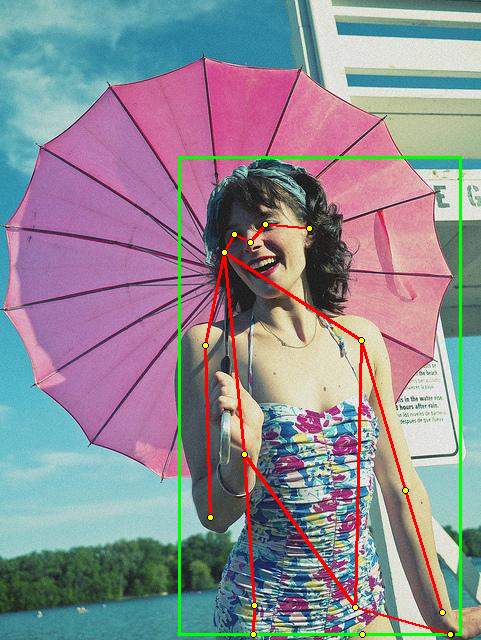
\includegraphics[width=\linewidth]{figures/demo_keypoints_overlay.png}
    \caption{\cmd{yolozu demo keypoints}}
  \end{subfigure}\hfill
  \begin{subfigure}[t]{0.32\linewidth}
    \centering
    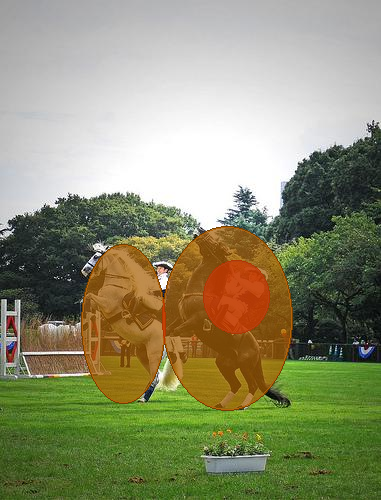
\includegraphics[width=\linewidth]{figures/demo_instance_seg_overlay.png}
    \caption{\cmd{yolozu demo instance-seg}}
  \end{subfigure}\hfill
  \begin{subfigure}[t]{0.32\linewidth}
    \centering
    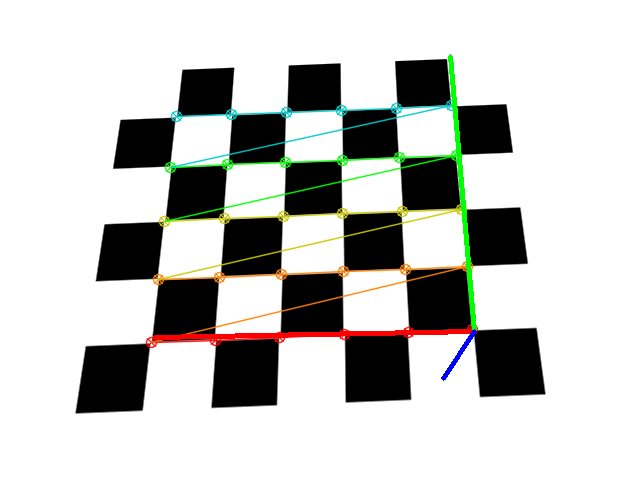
\includegraphics[width=\linewidth]{figures/demo_pose_overlay.png}
    \caption{\cmd{yolozu demo pose --backend aruco}}
  \end{subfigure}
  \caption{Real-image outputs from the keypoints, instance segmentation, and 6DoF pose demos. The tasks differ, but all stay aligned with the predictions interface contract mindset.}
\end{figure}

The corresponding commands are:
\begin{lstlisting}[language=bash]
python3 -m pip install -U 'yolozu[demo]'
yolozu demo keypoints
python3 scripts/download_coco_instances_tiny.py --out-root data/coco --split val2017 --num-images 8 --seed 0
yolozu demo instance-seg --background coco-instances --inference auto --num-images 1 --max-instances 8 --score-threshold 0.25
yolozu demo pose --backend aruco
\end{lstlisting}

To enable the COCO instances (polygon) background for the instance-seg demo without long flags:
\begin{lstlisting}[language=bash]
python3 scripts/download_coco_instances_tiny.py
yolozu demo instance-seg
\end{lstlisting}

To run a visible raw-versus-TTA comparison on a corrupted real COCO image:
\begin{lstlisting}[language=bash]
yolozu demo instance-seg-tta --run-dir reports/demo_instance_seg_tta
\end{lstlisting}

\noindent This writes \path{reports/demo_instance_seg_tta/selected/overlay_raw.png},
\path{reports/demo_instance_seg_tta/selected/overlay_tta.png}, and
\path{reports/demo_instance_seg_tta/instance_seg_tta_demo_report.json}.


\section{Source Checkout (Repository Path)}
If you are operating directly within the repository (e.g., utilizing the training stack or power-user scripts), follow this procedure:
\begin{lstlisting}[language=bash]
python3 -m pip install -r requirements-test.txt
python3 -m pip install -e .
python3 -m pytest -q
\end{lstlisting}

The repository-only smoke and fresh-install evidence harnesses require this checkout:
\begin{lstlisting}[language=bash]
bash scripts/smoke.sh
bash scripts/fresh_install_journey.sh --run-dir /tmp/yolozu_fresh_install
\end{lstlisting}
The fresh-install harness creates a new virtual environment, installs from public PyPI, and records
the resolved version, exact commands, exit codes, elapsed times, logs, and stable-lane reports.
Use a new run directory for each invocation.


\section{Recommended Deployment Flow}
The canonical deployment pipeline follows this progression:
\begin{quote}
PyTorch \(\to\) ONNX \(\to\) TensorRT
\end{quote}

On macOS, you can typically run CPU-bound tooling (validation, evaluation, and ONNX Runtime CPU export).
Treat MPS as available only when the local Torch runtime reports success for
\cmd{torch.backends.mps.is_available()}.
If that check is false, treat the machine as CPU-only for \yolozu{} purposes.
Python itself can still create the environment with \cmd{venv} and \cmd{pip}; when MPS does not come up, the usual blocker is the Torch wheel/runtime combination rather than Python environment creation. Miniforge/conda is therefore a fallback for some Apple Silicon hosts, not a hard requirement.
TensorRT execution is generally Linux/NVIDIA-centric.
TensorRT workflows are covered in the Real-Time vs. Batch Inference chapter. The canonical pipeline strictly follows PyTorch $\rightarrow$ ONNX $\rightarrow$ TensorRT and includes parity checks at each stage.

\begin{figure}[h]
\centering
\resizebox{\linewidth}{!}{%
\begin{tikzpicture}[
  node distance=8mm and 10mm,
  font=\small,
  box/.style={draw, rounded corners, align=left, inner sep=6pt},
  lane/.style={draw, rounded corners, inner sep=5pt, fill=gray!6},
  arrow/.style={-{Latex[length=2mm]}, thick},
  dashedarrow/.style={-{Latex[length=2mm]}, thick, dashed}
]

\node[box] (torch) {\textbf{PyTorch artifact}\\
train/checkpoint\\
\path{runs/<run_id>/checkpoints/*}};
\node[box, right=14mm of torch] (onnx) {\textbf{ONNX artifact}\\
\path{model.onnx}\\
\path{model.onnx.meta.json}};
\node[box, right=14mm of onnx] (trt) {\textbf{TensorRT artifact}\\
\path{engine.plan}\\
\path{engine.meta.json}};

\node[box, below=12mm of onnx] (export) {\textbf{Runtime adapter}\\
torch / onnxrt / opencv-dnn / trt};
\node[box, right=16mm of export] (pred) {\textbf{Prediction artifact}\\
\path{predictions.json}\\
schema-valid + relocatable\\
\cmd{meta.export_settings}};
\node[box, right=16mm of pred] (eval) {\textbf{Validation reports}\\
\path{eval_suite.json}\\
\path{metrics_report.json}};

\draw[arrow] (torch) -- (onnx);
\draw[arrow] (onnx) -- (trt);

\draw[dashedarrow] (torch) -- node[midway, left]{\scriptsize torch} (export);
\draw[dashedarrow] (onnx) -- node[midway, right]{\scriptsize onnxrt / opencv} (export);
\draw[dashedarrow] (trt) -- node[midway, right]{\scriptsize tensorrt} (export);

\draw[arrow] (export) -- (pred);
\draw[arrow] (pred) -- (eval);

\begin{pgfonlayer}{bg}
\node[lane, fit=(torch)(onnx)(trt), label=above:{\textbf{Artifacts}}] {};
\node[lane, fit=(export), label=below:{\textbf{Runtime}}] {};
\node[lane, fit=(pred)(eval), label=below:{\textbf{Validation}}] {};
\end{pgfonlayer}

\end{tikzpicture}
}
\caption{Recommended deployment flow, grouped by artifact creation, runtime adaptation, and validation evidence.}
\end{figure}
%

\chapter{Core Concepts and Interface Contracts}

\ChapterMeta{
This chapter elucidates the core interface contracts (schemas) and the dataset and prediction migration methodologies employed throughout the repository.
}{

It ensures evaluation stability across diverse backends and over time by mandating explicit, versionable inputs and outputs.
}{

This documentation assumes adherence to the specified schemas and treats generated wrapper artifacts (e.g., \path{dataset.json}) as integral components of the workflow.
}

\section{Contract-First Evaluation}
The interface contracts (schemas) are the foundational product of this repository. They empower you to:
\begin{itemize}
  \item Conduct equitable comparisons across disparate inference backends.
  \item Guarantee the reproducibility of evaluations over time.
  \item Maintain tooling stability, even as underlying models undergo architectural evolution.
\end{itemize}

Core interface contracts include:
\begin{itemize}
  \item \textbf{Predictions Schema}: \path{docs/predictions_schema.md}
  \item \textbf{Adapter interface contract}: \path{docs/adapter_contract.md}
  \item \textbf{Training run interface contract (Run Contract)}: \path{docs/run_contract.md}
  \item \textbf{SynthGen intake interface contract}: \path{docs/synthgen_contract.md}
\end{itemize}

\begin{figure}[h]
\centering
\resizebox{\linewidth}{!}{%
\begin{tikzpicture}[
  node distance=10mm,
  font=\small,
  box/.style={draw, rounded corners, align=left, inner sep=6pt},
  group/.style={draw, rounded corners, inner sep=8pt},
  arrow/.style={-{Latex[length=2mm]}, thick}
]

% Left to right: ingest -> adapter -> predictions -> eval
\node[box] (dataset) {\textbf{Dataset input}\\
\path{images/<split>/}, \path{labels/<split>/}\\
optional: \path{dataset.json}, \path{classes.json}};

\node[box, right=18mm of dataset] (adapter) {\textbf{Adapter / inference}\\
torch / onnxrt / trt / opencv-dnn\\
or external C++/Rust};

\node[box, right=18mm of adapter] (pred) {\textbf{Interface contract}\\
\path{predictions.json}\\
\texttt{meta.export\_settings}};

\node[box, right=18mm of pred] (eval) {\textbf{Validate \& evaluate}\\
schema validators\\
metrics reports};

\node[box, above=12mm of pred] (contracts) {\textbf{Other interface contracts}\\
adapter boundary\\
run artifacts\\
SynthGen intake};

% Connections
\draw[arrow] (dataset) -- (adapter);
\draw[arrow] (adapter) -- (pred);
\draw[arrow] (pred) -- (eval);
\draw[arrow] (contracts) -- (adapter);
\draw[arrow] (contracts) -- (pred);

% Group boxes
\node[group, fit=(dataset), label={[align=left]above:Ingest}] {};
\node[group, fit=(adapter), label={[align=left]above:Backends}] {};
\node[group, fit=(pred), label={[align=left]above:Stable I/O}] {};
\node[group, fit=(eval), label={[align=left]above:Common scoring}] {};

\end{tikzpicture}
}
\caption{YOLOZU uses stable interface contracts to decouple inference backends from evaluation.}
\end{figure}

When links and prose disagree, treat these interface contract documents as canonical and re-verify against \path{tools/manifest.json} and tool \cmd{--help} output.

\section{Datasets}
The majority of tools anticipate a YOLO-style dataset hierarchy (comprising \path{images/}, \path{labels/}, and splits), supplemented by optional metadata.
Supported image formats: JPEG (\texttt{.jpg}, \texttt{.jpeg}), PNG, BMP, TIFF (\texttt{.tif}, \texttt{.tiff}), WebP, and GIF.

\subsection{Frictionless Migration (Utilizing Datasets "As-Is")}
\yolozu{} is engineered to evaluate prevalent training ecosystems with minimal friction. The central paradigm is to circumvent manual dataset restructuring by generating lightweight \textbf{descriptor artifacts}.

In practice, migration commands yield:
\begin{itemize}
  \item A concise \path{dataset.json} wrapper (which references existing images and labels), and/or
  \item Converted label files (e.g., translating COCO JSON to YOLO text labels) accompanied by a wrapper.
\end{itemize}

The overarching objective is to preserve the integrity of source datasets while rendering evaluation inputs explicit and versionable.

\begin{figure}[h]
\centering
\resizebox{\linewidth}{!}{%
\begin{tikzpicture}[
  node distance=10mm,
  font=\small,
  box/.style={draw, rounded corners, align=left, inner sep=6pt},
  arrow/.style={-{Latex[length=2mm]}, thick}
]

\node[box] (ultra) {\textbf{Ultralytics}\\
\path{data.yaml}\\
\path{images/<split>/}};
\node[box, below=10mm of ultra] (coco) {\textbf{COCO dataset}\\
\path{instances\_*.json}\\
category\_id};
\node[box, below=10mm of coco] (extpred) {\textbf{External results}\\
COCO results JSON\\
or framework output};

\node[box, right=28mm of coco] (wrapper) {\textbf{Wrapper / mapping}\\
\path{dataset.json}\\
\path{classes.json}};
\node[box, right=28mm of extpred] (pred) {\textbf{predictions.json}\\
schema-valid\\
relocatable paths};
\node[box, right=22mm of wrapper] (eval) {\textbf{Validate \& eval}\\
same evaluator\\
same metrics};

\draw[arrow] (ultra) -- (wrapper);
\draw[arrow] (coco) -- node[midway, above, sloped]{\scriptsize convert labels} (wrapper);
\draw[arrow] (extpred) -- (pred);
\draw[arrow] (wrapper) -- (eval);
\draw[arrow] (pred) -- (eval);

\end{tikzpicture}
}
\caption{Migration map: keep native training ecosystems, convert only the interface boundary artifacts.}
\end{figure}

\subsection{Ultralytics Datasets (YOLOv8/YOLO11)}
If your dataset is already defined by an Ultralytics-style \path{data.yaml} (referencing \path{images/<split>/} and \path{labels/<split>/}), \yolozu{} can generate a lightweight \path{dataset.json} wrapper, leaving the original dataset entirely unmodified.

For precise command syntax and validation procedures, refer to Chapter~5 (Workflow~D: Migrate Datasets and Predictions).

\subsection{COCO JSON Datasets (Migration)}
Numerous ecosystems rely on COCO-style \path{instances_*.json} files for object detection. Because \yolozu{} consumes YOLO-style text labels, the supported migration trajectory is:
COCO JSON \texorpdfstring{$\rightarrow$}{->} YOLO labels + \path{dataset.json} wrapper.

For the specific conversion command, consult Chapter~5 (Workflow~D: Migrate Datasets and Predictions).

\subsection{Importing Predictions from External Ecosystems}
Frameworks such as Detectron2, MMDetection, and YOLOX frequently export detection results in COCO format. Typical fields include:
\begin{itemize}
  \item \cmd{image_id}
  \item \cmd{category_id}
  \item \cmd{box}
  \item \cmd{score}
\end{itemize}

\yolozu{} seamlessly converts these outputs into a compliant \path{predictions.json}:
\begin{lstlisting}[language=bash]
yolozu migrate predictions \
  --from coco-results \
  --results /path/to/coco_results.json \
  --instances /path/to/instances_val2017.json \
  --output reports/predictions.json \
  --force
\end{lstlisting}

Following conversion, proceed with standard validation and evaluation.

\subsection{External SynthGen intake contract}
For synthetic data pipelines, \yolozu{} intentionally limits scope to \textbf{intake and evaluation}; generation remains in an external repository.
The intake boundary is fixed by \path{docs/synthgen_contract.md} and \path{schemas/synthgen_sample.schema.json}, with required fields such as \cmd{image}, \cmd{depth\_ndc}, \cmd{inst\_id}, \cmd{sem\_id}, and \cmd{kpts2d}.

Validate shard metadata before training/evaluation:
\begin{lstlisting}[language=bash]
python3 tools/validate_synthgen_contract.py \
  --input /path/to/synthgen_dataset/shards/train_000.jsonl \
  --max-samples 200
\end{lstlisting}

\section{Predictions JSON}
A predictions artifact typically manifests as a JSON array containing per-image objects. While the precise structure varies by task (e.g., bounding box, segmentation, pose estimation), the guiding principles remain constant:
\begin{itemize}
  \item \textbf{Stability}: Keys and data types are strictly schema-validated.
  \item \textbf{Portability}: File paths are relative and relocatable wherever feasible.
  \item \textbf{Traceability}: Metadata (such as run ID, Git SHA, and environment details) is embedded alongside the results.
\end{itemize}

To rigorously validate a predictions artifact:
\begin{lstlisting}[language=bash]
python3 tools/validate_predictions.py /path/to/predictions.json --strict
\end{lstlisting}

\section{Adapters (Bring-Your-Own Inference)}
An adapter functions as a thin interface layer bridging a specific inference implementation and \yolozu{}'s standardized interface contracts. If your system can generate a compliant \path{predictions.json}, it can be evaluated.

In practical terms, this entails:
\begin{itemize}
  \item \textbf{Input}: Dataset records supply an \cmd{image} path (and optional label/sidecar metadata).
  \item \textbf{Output}: Per-image \cmd{detections} must include \cmd{class_id}, \cmd{score}, and \cmd{box} (typically formatted as \cmd{cxcywh_norm}), alongside any task-specific optional fields.
  \item \textbf{Validation}: It is imperative to execute \cmd{tools/validate_predictions.py --strict} prior to evaluation.
\end{itemize}

\section{Reports and Reproducibility}
The majority of workflows are architected to emit:
\begin{itemize}
  \item Machine-readable JSON reports.
  \item Optional HTML overlays for visual debugging.
  \item Stable artifact nomenclature within a designated run directory.
\end{itemize}

This design is highly intentional: it streamlines regression testing and facilitates effortless cross-run comparisons.

\chapter{CLI Reference (Practical)}

\ChapterMeta{
This chapter provides a concise summary of the most frequently utilized commands and demonstrates how to explore the complete Command Line Interface (CLI) surface via the \cmd{--help} flag.
}{
It is designed to minimize the time to first execution and to clearly delineate which commands are install-safe versus those restricted to repository-only workflows.
}{
Utilize \cmd{yolozu --help} for the pip-installed CLI, or \cmd{python3 tools/yolozu.py --help} for the repository wrapper. Because implementation details evolve, the \cmd{--help} output remains the definitive source of truth.
}
\ChapterAudience{Read this chapter when you want copy-paste entrypoints first and detailed tool discovery second.}


\section{Design Philosophy}
The CLI surface is intentionally bifurcated to serve distinct user profiles:
\begin{itemize}
  \item \cmd{yolozu}: The end-user safe CLI, installed globally or virtually via pip.
  \item \cmd{python3 tools/yolozu.py}: The repository wrapper, specifically tailored for research and evaluation pipelines.
\end{itemize}

This chapter documents the \textit{high-traffic commands} and outlines the methodology for discovering the broader command set.

\section{Discoverability}
As a best practice, always initiate discovery with:\\
\cmd{yolozu --help} and \cmd{yolozu <command> --help}.\\
For repository-specific workflows, utilize: \cmd{python3 tools/yolozu.py --help}.

\section{Common Commands}
\begin{longtable}{@{}p{0.40\textwidth}p{0.55\textwidth}@{}}
\toprule
\textbf{Command} & \textbf{Purpose} \\
\midrule
\cmd{yolozu doctor} & Executes environment diagnostics (verifying dependencies, GPU status, and backend availability). \\
\cmd{yolozu completion} & Prints shell completion scripts (\cmd{--shell bash|zsh}) for interactive command completion. \\
\cmd{yolozu demo overview} & Writes a demo overview report (\path{demo\_output/overview/...}) covering bbox/segmentation/keypoints/depth/pose6d flows, dependency checks, and recommended commands. \\
\cmd{yolozu demo} & Runs a small CPU-friendly demo suite and writes artifacts under \path{demo\_output/}. \\
\cmd{yolozu demo instance-seg} & Instance-seg demo (offline by default). \newline
For real-image overlays: \cmd{--background yolo-bbox --yolo-root data/smoke --yolo-split val --inference none}. \newline
For polygon masks/inference: \cmd{--background coco-instances}. \\
\cmd{yolozu demo instance-seg-tta} & Real-image instance-seg TTA compare demo. Scans a small COCO polygon subset, applies a deterministic corruption, then writes raw-vs-augmentation-based-TTA overlays under \path{demo\_output/instance\_seg\_tta/} or the chosen \cmd{--run-dir}. \\
\cmd{yolozu demo keypoints} & Keypoint R-CNN inference demo (torchvision; writes overlay under \path{demo\_output/keypoints/}). \\
\cmd{yolozu demo pose} & 6D pose demo (chessboard/ArUco by default; ArUco sample cached under \path{demo\_output/pose/\_samples/}; DenseFusion requires CUDA + large downloads). Writes overlay under \path{demo\_output/pose/}. \\
\cmd{yolozu demo depth} & Monocular depth inference demo (default: Depth Anything via Transformers; optional MiDaS/DPT; writes images under \path{demo\_output/depth/}). \\
\cmd{yolozu demo train} & Training demo (MNIST fine-tune; bounded by \cmd{--max-steps}; downloads ResNet18 on first run; writes under \path{demo\_output/train/}). \\
\cmd{yolozu demo continual} & Continual-learning demo (toy synthetic by default; \cmd{--problem mnist\_rotate} uses a vision backbone). \\
\cmd{yolozu list models} & Lists curated model IDs available for reproducible downloads. \\
\cmd{yolozu fetch <model\_id> --accept-license} & Downloads a model artifact with cache reuse, sha256 verification, and license gating; records \path{models/<id>/meta.json}. (Custom registries may require \cmd{--allow-unsafe} / \cmd{--allow-non-apache}.) \\
\cmd{bash scripts/smoke.sh} & Runs the one-command offline smoke flow (doctor + validate + eval-coco dry-run + SynthGen intake smoke + instance-seg overlay PNG evidence on \path{data/smoke}). \\
\cmd{bash scripts/smoke.sh --profile deep} & Runs the deep walkthrough profile and writes \path{reports/smoke\_walkthrough\_report.json} plus backend dry-run export artifacts. \\
\cmd{bash scripts/smoke.sh --help} & Shows smoke CLI options (\cmd{--dataset}, \cmd{--predictions}, \cmd{--report}, \cmd{--synthgen-root}, \cmd{--synthgen-predictions}, \cmd{--output-dir}, \cmd{--demo-run-dir}, \cmd{--skip-demo}, \cmd{--torch-device}, \cmd{--profile}, \cmd{--walkthrough-report}). \\
\cmd{bash scripts/ttt\_compare.sh} & Short baseline-vs-adapted TTT compare wrapper. Use \cmd{--boilerplate tent|mim|mim\_probe|cotta|eata|sar} plus \cmd{--dataset}, \cmd{--checkpoint}, and \cmd{--run-dir}; it writes baseline/adapted predictions and a before-after Markdown+JSON summary. \\
\cmd{yolozu train} & Initiates YAML/JSON config-driven RT-DETR training (fully supporting the run contract and resumption capabilities). \\
\cmd{yolozu test} & Executes the YAML/JSON scenario runner (compatible with dummy, precomputed, and rtdetr\_pose adapters). \\
\cmd{yolozu predict-images} & Performs folder-level inference, generating predictions, visual overlays, and an HTML summary. \\
\cmd{yolozu eval-coco} & Conducts COCO mAP evaluation derived from \path{predictions.json} (requires COCO tooling to be installed). \\
\cmd{yolozu benchmark} & Parity-target benchmark entrypoint. Runs real backend orchestration for \cmd{torch}/\cmd{onnx}/\cmd{engine} when artifacts and runtimes exist, otherwise records explicit skipped/placeholder results. Key knobs include \cmd{--protocol}, backend-specific model overrides (\cmd{--torch-model}, \cmd{--onnx-model}, \cmd{--engine-model}), and \cmd{--latency-source auto}. \\
\cmd{yolozu parity} & Compares two distinct predictions artifacts to detect backend drift or discrepancies. \\
\cmd{yolozu predictions migrate} & Migrates predictions entry schema versions (currently \cmd{--from v1 --to v2}) with optional strict source checking. \\
\cmd{yolozu calibrate} & Applies score calibration and long-tail post-hoc adjustments. \\
\cmd{yolozu long-tail-recipe} & Generates a long-tail training recipe JSON with selectable sampler/loss/metric/lr scheduler plugins. \\
\cmd{python3 tools/eval_suite.py} & Executes suite evaluation, providing protocol-pinned reporting and cross-run comparisons. \\
\cmd{python3 tools/run\_reference\_adapter\_regression.py} & Runs RT-DETR reference-adapter regression with profile-aware micro/full modes, interface contract gates (hard), behavior/parity gates (warn/hard), deterministic-preprocess metadata checks, provenance snapshot capture (\cmd{--capture-provenance}), matrix baseline layout (\cmd{--baseline-layout matrix}), lock/hash enforcement, and failure artifacts (\cmd{--diff-summary-out}, \cmd{--topk-examples-dir}). \\
\cmd{python3 tools/hpo_sweep.py} & Orchestrates hyperparameter sweeps and aggregates metrics into CSV, MD, or JSONL formats. \\
\cmd{python3 tools/benchmark\_model.py} & Repository wrapper for \cmd{yolozu benchmark}; useful when backend-specific benchmark behavior must also be tracked in \path{tools/manifest.json}. \\
\cmd{python3 tools/run\_ttt\_compare.py} & Python entrypoint for the same TTT compare workflow; loads method boilerplates from \path{configs/examples/ttt\_compare/} and writes `plan.json`, before/after predictions, optional eval reports, and compare summaries. \\
\cmd{python3 tools/render\_ttt\_manual\_figures.py} & Renders the checked-in TTT summary/workflow/qualitative PNG figures from fixed report artifacts for \path{docs/assets/} and \path{manual/figures/}. \\
\cmd{python3 tools/benchmark_latency.py} & Runs the latency/FPS benchmark harness, maintaining a JSONL history to track performance regressions. \\
\cmd{python3 tools/check\_repo\_governance.py} & Audits local governance evidence plus exported GitHub settings snapshots for branch protection, review policy, and repository-security posture. Writes a JSON summary and keeps history-based items explicit instead of pretending they are source-only facts. \\
\cmd{python3 tools/validate_tool_manifest.py} & Validates the structural integrity of the machine-readable registry (\path{tools/manifest.json}). \\
\cmd{bash release.sh} & Runs no-option release automation: auto SemVer/CalVer version bump policy, tag push, GitHub release publish, and PyPI/Zenodo workflow handoff. \\
\cmd{python3 tools/support\_yolo\_detr.py} & YOLO/DETR support utility with fixed 3-layer interface contract (trainer/repo/export), short aliases (\cmd{ls/tu/th/eo/pn}), preset defaults (\cmd{-P smoke}), shared dataset conversion, ONNX export templates, and prediction canonicalization. \\
\bottomrule
\end{longtable}

\section{Demo Output Examples (Images)}
The \cmd{yolozu demo *} commands are designed to produce concrete artifacts (JSON reports and overlay images)
that help users verify they can run end-to-end workflows.

The figures below are committed snapshots generated from \path{data/smoke} using the following commands:
\begin{lstlisting}[language=bash]
yolozu demo instance-seg \
  --background yolo-bbox --yolo-root data/smoke --yolo-split val --inference none \
  --num-images 1 --image-size 320 --max-instances 3 \
  --run-dir demo_output/manual/instance_seg

yolozu demo keypoints \
  --image data/smoke/images/val/000000000036.jpg --device cpu --max-persons 1 \
  --run-dir demo_output/manual/keypoints

yolozu demo depth \
  --image data/smoke/images/val/000000000036.jpg --device cpu --model midas_small \
  --run-dir demo_output/manual/depth

yolozu demo pose \
  --backend chessboard --sample-source synthetic \
  --run-dir demo_output/manual/pose
\end{lstlisting}

\begin{figure}[htbp]
  \centering
  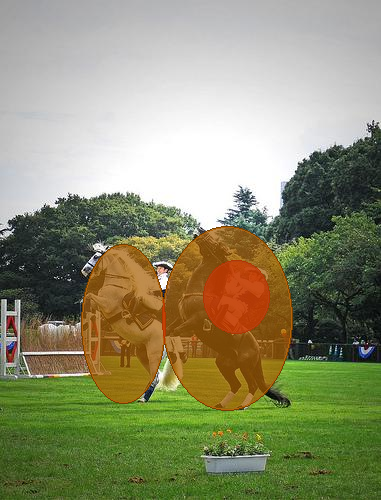
\includegraphics[width=0.95\textwidth]{figures/demo_instance_seg_overlay.png}
  \caption{Instance-seg demo overlay (\cmd{--background yolo-bbox --inference none}). This offline mode uses GT-derived scaffold predictions for visualization and evaluation smoke checks.}
\end{figure}

\begin{figure}[htbp]
  \centering
  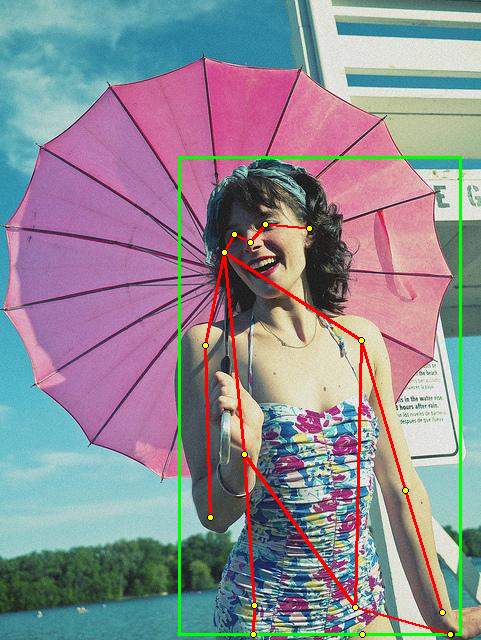
\includegraphics[width=0.95\textwidth]{figures/demo_keypoints_overlay.png}
  \caption{Keypoints demo overlay (torchvision Keypoint R-CNN).}
\end{figure}

\begin{figure}[htbp]
  \centering
  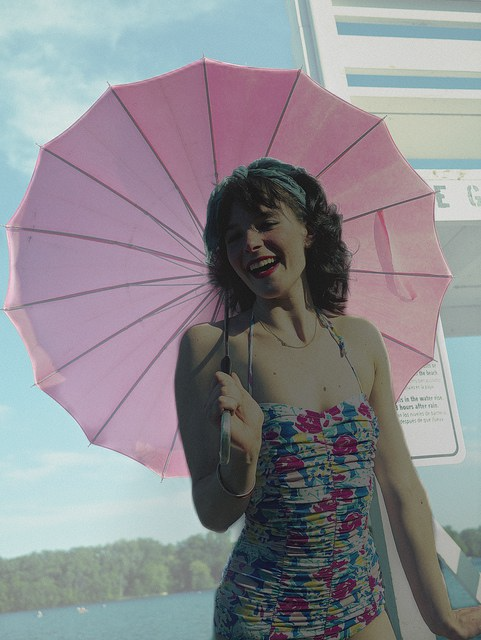
\includegraphics[width=0.95\textwidth]{figures/demo_depth_overlay.png}
  \caption{Depth demo overlay (MiDaS small; relative depth visualization).}
\end{figure}

\begin{figure}[htbp]
  \centering
  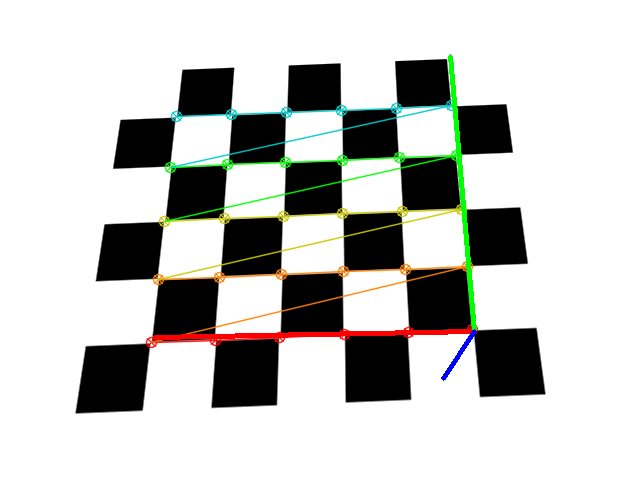
\includegraphics[width=0.95\textwidth]{figures/demo_pose_overlay.png}
  \caption{Pose6D demo overlay (chessboard + OpenCV solvePnP).}
\end{figure}

\subsection{Long-tail recipe plugin options (PyTorch)}
\cmd{yolozu long-tail-recipe} supports explicit plugin choices for loss, validation metric, and learning-rate scheduler.

\begin{lstlisting}[language=bash]
yolozu long-tail-recipe \
  --dataset data/smoke --split val \
  --loss-plugin torch_cross_entropy \
  --metric-plugin torch_top1_accuracy \
  --lr-scheduler torch_step_lr \
  --output reports/long_tail_recipe_torch.json --force
\end{lstlisting}

Primary plugin flags:
\begin{itemize}
  \item \cmd{--loss-plugin}: \cmd{none}, \cmd{focal}, \cmd{ldam}, \cmd{torch\_cross\_entropy}, \cmd{torch\_nll\_loss}, \cmd{torch\_bce\_with\_logits}
  \item \cmd{--metric-plugin}: \cmd{none}, \cmd{torch\_top1\_accuracy}, \cmd{torch\_top5\_accuracy}, \cmd{torch\_cross\_entropy}
  \item \cmd{--lr-scheduler}: \cmd{none}, \cmd{torch\_step\_lr}, \cmd{torch\_cosine\_annealing\_lr}, \cmd{torch\_reduce\_on\_plateau}, \cmd{torch\_one\_cycle\_lr}
\end{itemize}

\section{YAML Config-Driven Usage (Train/Test/Resume)}
\yolozu{} supports the ingestion of a YAML or JSON configuration file as its primary positional argument.
Internally, \cmd{yolozu train} delegates the \cmd{--config <file>} argument to \path{rtdetr_pose.train_minimal}, whereas \cmd{yolozu test} maps YAML keys directly to \path{yolozu.scenarios_cli} arguments.

\begin{longtable}{@{}p{0.18\textwidth}p{0.30\textwidth}p{0.46\textwidth}@{}}
\toprule
\textbf{Use Case} & \textbf{YAML File} & \textbf{Command Pattern} \\
\midrule
Train (Default) & \path{configs/examples/train_setting.yaml} & \cmd{yolozu train <train_setting.yaml>} \\
Train (Contract) & \path{configs/examples/train_contract.yaml} & \cmd{yolozu train <train_contract.yaml> --run-id <id>} \\
Resume & Same as Train (Contract) & \cmd{yolozu train <train_contract.yaml> --run-id <id> --resume} \\
Test (Scenario) & \path{configs/examples/test_setting.yaml} & \cmd{yolozu test <test_setting.yaml> [test_args...]} \\
\bottomrule
\end{longtable}

Concrete execution examples:
\begin{lstlisting}[language=bash]
yolozu train configs/examples/train_setting.yaml
yolozu train configs/examples/train_contract.yaml --run-id exp01
yolozu train configs/examples/train_contract.yaml --run-id exp01 --resume
yolozu test configs/examples/test_setting.yaml --adapter precomputed --predictions reports/predictions.json
\end{lstlisting}

Backbone substitutions are governed exclusively by the model configuration JSON, rather than by modifying adapter commands directly:
\begin{lstlisting}[language=bash]
yolozu train configs/examples/train_setting.yaml \
  --model-config rtdetr_pose/configs/base.json
\end{lstlisting}

For comprehensive details regarding the backbone contract and supported architectures, refer to \path{docs/backbones.md}.

\subsection{Test YAML and the Override Rule}
The default test YAML configuration is intentionally minimalist (typically specifying only the adapter, dataset, split, and max\_images). Runtime-specific parameters are conventionally supplied as CLI overrides:
\begin{lstlisting}[language=bash]
yolozu test configs/examples/test_setting.yaml \
  --adapter rtdetr_pose \
  --config rtdetr_pose/configs/base.json \
  --checkpoint /path/to/checkpoint.pt \
  --dataset data/smoke \
  --max-images 50
\end{lstlisting}

\noindent This paradigm directly mirrors the documented real-model workflow detailed in \path{docs/real_model_interface.md}.

\section{Repository Power Tools}
A multitude of task-specific scripts are housed within the \path{tools/} directory. Notable examples include:
\begin{itemize}
  \item \path{tools/validate_predictions.py}
  \item \path{tools/eval_instance_segmentation.py}
  \item \path{tools/eval_segmentation.py}
  \item \path{tools/export_predictions.py} (Facilitates adapter-based export)
\end{itemize}

For an exhaustive inventory, consult \path{tools/manifest.json} (for machine-readable metadata) and the documentation index (for human-readable guidance).

\chapter{Troubleshooting}

\ChapterMeta{
This chapter provides an accelerated debugging playbook: it emphasizes validating artifacts first, followed by investigating common integration failure modes.
}{
Adhering to this playbook drastically shortens iteration times by identifying schema violations, pathing errors, and class-mapping discrepancies before you attempt to interpret potentially flawed metrics.
}{
It is most effective when validators are executed on the exact artifacts slated for evaluation. Pay meticulous attention to the \cmd{--pred-root} parameter and ensure consistent class ordering between the exporter and the evaluator.
}
\ChapterAudience{Read this chapter when results look wrong and you want the shortest route to the first likely failure point.}


\section{Validate early and often}
If evaluation results appear anomalous, your immediate first step must be artifact validation.

To validate the standard predictions schema:
\begin{lstlisting}[language=bash]
python3 tools/validate_predictions.py /path/to/predictions.json --strict
\end{lstlisting}

To validate instance segmentation predictions:
\begin{lstlisting}[language=bash]
python3 tools/validate_instance_segmentation_predictions.py /path/to/preds.json
\end{lstlisting}

\section{Common failure modes}
\begin{itemize}
  \item \textbf{Pathing issues}: Relative paths embedded within the JSON artifact fail to resolve correctly against the specified \cmd{--pred-root}.
  \item \textbf{Class mapping mismatches}: The ordering defined in \path{classes.txt} diverges from the internal mapping utilized by the model or exporter.
  \item \textbf{Backend discrepancies}: Pre-processing or post-processing logic varies subtly across different inference backends.
  \item \textbf{TensorRT environment constraints}: TensorRT execution is strictly pinned to Linux/NVIDIA environments; use the documented container workflow to keep CUDA/TRT/ORT compatibility pinned.
  \item \textbf{CI scope optimization}: Required CI uses a change-scope fast path; docs/metadata-only commits skip heavy test jobs by design.
  \item \textbf{Container workflow expectations}: \path{.github/workflows/container.yml} now builds container-related pull requests for early validation, while image publication remains gated to tag/manual runs. Manual republishes should pass \texttt{release\_tag=vX.Y.Z}; when \texttt{NGC\_API\_KEY} is configured, the same workflow mirrors images to \path{nvcr.io/yolozu/...}.
  \item \textbf{Container trigger scope}: Container checks on pull requests and \texttt{main} pushes stay restricted to container-related paths (workflow/deploy/packaging inputs) to avoid unnecessary runs.
  \item \textbf{Security scan backlog vs real regressions}: \path{.github/workflows/codeql.yml} and \path{.github/workflows/scorecard.yml} report repository posture, not just runtime test failures. Scorecard also runs on pull requests targeting \texttt{main}, so posture regressions should surface before merge rather than only after landing on the default branch.
  \item \textbf{Fuzzing coverage expectations}: \path{.github/workflows/cflite\_pr.yml} and \path{.github/workflows/cflite\_batch.yml} exercise predictions normalization via ClusterFuzzLite. When predictions parsing/canonicalization changes, update \path{.clusterfuzzlite/} and \path{fuzz/} in the same pull request.
  \item \textbf{Self-hosted GPU workflow behavior}: \path{.github/workflows/ngc_test.yml} probes for an idle \texttt{self-hosted + gpu} runner first; if none is online/idle, the workflow exits via a deterministic skip job. If probe API access is denied (\texttt{403}), configure repository secret \texttt{RUNNER\_DISCOVERY\_TOKEN} to enable runner discovery.
  \item \textbf{ONNXRuntime model-load failures}: If ORT reports unsupported ONNX IR versions, regenerate artifacts with a compatible IR version (CI smoke pins IR v11 for compatibility).
\end{itemize}

\section{Further reading and resources}
\begin{itemize}
  \item Tools index: \path{docs/tools_index.md}
  \item External inference documentation: \path{docs/external_inference.md}
  \item Predictions schema specification: \path{docs/predictions_schema.md}
  \item Training and export overview: \path{docs/training_inference_export.md}
  \item CI incident logbook: \path{docs/ci_incidents.md}
  \item Release reliability checklist: \path{docs/release_reliability_checklist.md}
  \item Security and cryptography scope note: \path{docs/security_crypto_scope.md}
\end{itemize}


\part{Production Evaluation Manual}
\chapter{Workflows: Evaluate and Export}

\ChapterMeta{
This chapter outlines the canonical workflows for evaluating existing artifacts, exporting predictions from a backend, and executing convenient folder-level inference.
}{
It standardizes the generation of \path{predictions.json} and evaluation reports, ensuring that results remain strictly comparable and highly automatable.
}{
You will require a dataset root and one or more prediction artifacts; backend-specific operations may necessitate additional dependencies.
}
\ChapterAudience{Read this chapter when you already have data or model outputs and need to decide the fastest safe path to evaluation, export, or migration.}

\WorkflowOpening
{Pick the shortest route from existing outputs, backend inference, folder inference, or migration to a validated evaluation report.}
{Use this when you need to evaluate \path{predictions.json}, export one from a backend, inspect folder-level overlays, or normalize data from another ecosystem.}
{A dataset root or image folder; optionally an existing \path{predictions.json}, model artifact, backend runtime, or native dataset definition.}
{\cmd{yolozu validate predictions ... --strict} first, then the matching eval/export/migrate command for Workflow A--D.}
{\path{predictions.json}, validation output, evaluation JSON/HTML, overlays, or normalized dataset wrappers depending on the workflow.}
{Open the report JSON, confirm schema validation passed, and check that dataset split, class ids, and prediction counts match the intended run.}
{Missing files, stale relative paths, class-id drift, backend runtime imports, unsupported model shapes, or conceptual examples copied without real paths.}

\paragraph{Readiness classification.}
Workflow A in this chapter is the \textbf{stable main production lane} for \yolozu{}: validate predictions, then evaluate them under one pinned predictions interface contract.
Export paths and backend-specific execution remain useful, but they should be understood as secondary to that main lane.
See \path{docs/production_readiness.md}.

\paragraph{The shortest human summary.}
Most people arrive here with one of four questions:
\begin{itemize}
  \item ``I already have predictions. How do I evaluate them?''
  \item ``I have a model and a dataset. How do I export predictions safely?''
  \item ``I just want quick image-folder inference and overlays.''
  \item ``My data lives in another ecosystem. How do I migrate without rewriting everything?''
\end{itemize}

This chapter is organized exactly around those four questions.

\paragraph{Fast chooser.}
If you are unsure where to start:
\begin{itemize}
  \item choose \textbf{Workflow A} when inference already happened elsewhere,
  \item choose \textbf{Workflow B} when you need \yolozu{} to run inference and emit the standardized artifact,
  \item choose \textbf{Workflow C} when you want the quickest folder-level visual result,
  \item choose \textbf{Workflow D} when the problem is data or prediction migration rather than model execution.
\end{itemize}

\begin{figure}[h]
\centering
\resizebox{\linewidth}{!}{%
\begin{tikzpicture}[
  node distance=8mm,
  font=\small,
  box/.style={draw, rounded corners, align=left, inner sep=5pt},
  arrow/.style={-{Latex[length=2mm]}, thick}
]

% Row A
\node[box] (a_in) {\textbf{A}\\existing\\\path{predictions.json}};
\node[box, right=12mm of a_in] (a_val) {validate\\(\cmd{--strict})};
\node[box, right=12mm of a_val] (a_eval) {eval\\(suite / COCO)};
\node[box, right=12mm of a_eval] (a_rep) {reports\\JSON/HTML};
\draw[arrow] (a_in) -- (a_val);
\draw[arrow] (a_val) -- (a_eval);
\draw[arrow] (a_eval) -- (a_rep);

% Row B
\node[box, below=10mm of a_in] (b_in) {\textbf{B}\\backend\\inference};
\node[box, right=12mm of b_in] (b_exp) {export\\\path{predictions.json}\\+\cmd{export_settings}};
\node[box, right=12mm of b_exp] (b_val) {validate};
\node[box, right=12mm of b_val] (b_rep) {eval + reports};
\draw[arrow] (b_in) -- (b_exp);
\draw[arrow] (b_exp) -- (b_val);
\draw[arrow] (b_val) -- (b_rep);

% Row C
\node[box, below=10mm of b_in] (c_in) {\textbf{C}\\image folder\\or split};
\node[box, right=12mm of c_in] (c_run) {\cmd{predict-images}\\(+ overlays)};
\node[box, right=12mm of c_run] (c_out) {\path{predictions.json}\\+ HTML summary};
\draw[arrow] (c_in) -- (c_run);
\draw[arrow] (c_run) -- (c_out);

% Row D
\node[box, below=10mm of c_in] (d_in) {\textbf{D}\\dataset defs\\\path{data.yaml}/COCO};
\node[box, right=12mm of d_in] (d_mig) {migrate\\\path{dataset.json}\\labels/classes};
\node[box, right=12mm of d_mig] (d_out) {\path{predictions.json}\\(converted/exported)};
\node[box, right=12mm of d_out] (d_rep) {validate + eval};
\draw[arrow] (d_in) -- (d_mig);
\draw[arrow] (d_mig) -- (d_out);
\draw[arrow] (d_out) -- (d_rep);

\end{tikzpicture}
}
\caption{Workflow overview (A--D): keep inference flexible, fix the interface boundary at \cmd{predictions.json}.}
\end{figure}


\section{Workflow A: Evaluate existing predictions.json}
This is the safest and simplest path when a different system already produced model outputs.
You do not need to rerun inference; you only need a valid predictions artifact and a dataset root.

If you have already generated a \path{predictions.json} artifact from any inference backend, you can evaluate it directly:
\begin{lstlisting}[language=bash]
yolozu validate predictions /path/to/predictions.json --strict
python3 tools/eval_suite.py --dataset /path/to/yolo-dataset --predictions-glob '/path/to/predictions.json'
\end{lstlisting}

This represents the most common integration pathway for external inference systems.

\section{Workflow B: Run inference and export predictions}
Choose this path when you want \yolozu{} to be the boundary that turns backend-specific execution into a stable predictions artifact.

Depending on your deployment environment, several backends are available:
\begin{itemize}
  \item \textbf{Torch backend (research):} Exports predictions directly from a training checkpoint.
  \item \textbf{ONNX Runtime:} Facilitates CPU-friendly exports and rigorous parity checks.
  \item \textbf{OpenCV DNN (YOLO head):} Alternative ONNX execution via OpenCV DNN.
  \item \textbf{OpenCV DNN (RT-DETR, no NMS):} Logits+boxes decode path for RT-DETR ONNX (CUDA/CPU).
  \item \textbf{TensorRT:} Provides a pinned Linux/NVIDIA pipeline optimized for maximum throughput.
\end{itemize}

For production-oriented external inference, see \path{docs/external_inference.md} and the submodule-ready templates:
\path{examples/infer_cpp/} (CMake) and \path{examples/infer_rust/} (Rust).

\subsection{Rust template: optional ONNXRuntime mode}
The Rust template defaults to a minimal no-dependency interface-contract example, and can optionally enable ONNXRuntime via Cargo feature flags:
\begin{lstlisting}[language=bash]
# Minimal contract example (always available)
cargo build --release --manifest-path examples/infer_rust/Cargo.toml
examples/infer_rust/target/release/yolozu_infer_rust --out reports/pred_rust_stub.json

# Optional ONNXRuntime mode
cargo build --release --features onnxruntime --manifest-path examples/infer_rust/Cargo.toml
examples/infer_rust/target/release/yolozu_infer_rust \
  --mode onnxrt \
  --onnx /abs/path/model.onnx \
  --input-shape 1,3,64,64 \
  --image images/val/000001.jpg \
  --out reports/pred_rust_onnxrt.json
\end{lstlisting}

\noindent\textbf{Environment note:} The ONNXRuntime feature is intended for pinned Linux production images where Rust toolchains and ONNXRuntime shared libraries are provisioned explicitly.

\textbf{Conceptual (not copy-paste as-is):} repository-wrapper export shape.
Use real paths from \path{python3 -m yolozu export --help} for execution.
\begin{lstlisting}[language=bash]
# ONNXRuntime backend (input shape must match ONNX)
python3 -m yolozu export --backend onnxrt --dataset /path/to/yolo-dataset --split val --onnx /path/to/model.onnx --output reports/predictions.json

# TorchScript detection artifact with declared combined-output decode
python3 tools/export_predictions_torchscript.py --dataset /path/to/yolo-dataset --split val --model /path/to/model.torchscript --output reports/pred_torchscript.json --wrap

# ExecuTorch backend (.pte model; dry-run available for interface contract checks)
python3 -m yolozu export --backend executorch --dataset /path/to/yolo-dataset --split val --model /path/to/model.pte --output reports/pred_executorch.json --dry-run

# ExecuTorch non-dry decode: run ExecuTorch externally, then decode runtime rows
python3 -m yolozu export --backend executorch --dataset /path/to/yolo-dataset --split val --model /path/to/model.pte --runtime-output-json reports/executorch_runtime_outputs.json --boxes-scale norm --output reports/pred_executorch.json --force

# OpenCV DNN unified backend (auto decode + preset preprocess + IO dump)
python3 -m yolozu export --backend opencv-dnn --onnx /path/to/model.onnx --dataset /path/to/yolo-dataset --split val --max-images 8 --imgsz 640 --preprocess yolo_letterbox_640 --decode auto --dump-io reports/opencv_dump_io.json --output reports/pred_opencv_dnn_unified.json --force

# OpenCV DNN RT-DETR backend (no NMS)
python3 -m yolozu export --backend opencv-dnn-rtdetr --onnx /path/to/rtdetr.onnx --dataset /path/to/yolo-dataset --imgsz 640 --score-thr 0.01 --output reports/pred_rtdetr_opencv_backend.json --force

# OpenCV DNN YOLO backend (with NMS)
python3 -m yolozu export --backend opencv-dnn-yolo --onnx /path/to/yolo.onnx --dataset /path/to/yolo-dataset --imgsz 640 --score-thr 0.25 --nms-iou 0.45 --output reports/pred_opencv_dnn_yolo.json --force
\end{lstlisting}

For further details, consult:\\
\path{docs/training_inference_export.md}, \path{docs/external_inference.md}, and \path{docs/opencv_dnn_inference.md}.
For CI command-surface checks, prefer each exporter's \cmd{--dry-run} mode so schema and metadata contracts are validated without heavyweight runtime dependencies.

ExecuTorch non-dry mode intentionally does not pretend to execute a generic
mobile runtime inside YOLOZU. The declared path is: execute the \path{.pte}
artifact in the target ExecuTorch environment, write rows shaped
\cmd{[x1,y1,x2,y2,score,class_id]}, and pass that JSON via
\cmd{--runtime-output-json}. Unsupported row shapes fail before a predictions
artifact is written.

\subsection{Model intake before export (registry fetch)}
To standardize external checkpoints before running exporters, use the model fetch flow:
\begin{lstlisting}[language=bash]
yolozu list models
yolozu fetch yolox-s-coco --out models --accept-license
cat models/yolox-s-coco/meta.json
\end{lstlisting}

The generated \path{models/<id>/meta.json} always includes \path{source}, \path{version}, \path{license}, \path{sha256}, and \path{created_at}.

\subsection{YOLO user migration entrypoint (v5/v8/11/26)}
For users already operating within YOLO-family pipelines, \yolozu{} provides a direct interface-contract-first migration path:
\begin{lstlisting}[language=bash]
python3 tools/import_yolo_data_yaml.py --data-yaml /path/to/data.yaml --split val --output data/yolo_wrapper --force
python3 tools/export_predictions_yolo_runtime.py --model yolo11n.pt --dataset data/yolo_wrapper --split val --protocol nms_applied --wrap --output reports/pred_yolo_runtime.json
python3 tools/export_predictions_yolov5.py --dataset data/yolo_wrapper --split val --labels-dir runs/detect/exp/labels --protocol nms_applied --output reports/pred_yolov5.json
\end{lstlisting}

Protocol policy for fair comparisons:
\begin{itemize}
  \item \texttt{nms\_applied}: intended for YOLOv5/YOLOv8/YOLO11 post-NMS outputs.
  \item \texttt{e2e\_nms\_free}: intended for YOLO26/RT-DETR no-NMS outputs.
\end{itemize}

When outputs contain COCO \texttt{category\_id}, evaluate with class-id normalization:
\begin{lstlisting}[language=bash]
yolozu eval-coco --dataset data/yolo_wrapper --split val --predictions reports/pred_yolo_runtime.json --protocol nms_applied --classes data/yolo_wrapper/labels/val/classes.json --output reports/coco_eval_yolo_runtime.json
\end{lstlisting}

\subsection{YOLOX interoperability path}
For teams already operating YOLOX experiments (\path{exp.py} + checkpoints), keep native inference and export directly to the YOLOZU contract:
\begin{lstlisting}[language=bash]
python3 -m yolozu export --backend yolox --dataset /path/to/coco-yolo --split val2017 --exp /path/to/yolox_exp.py --weights /path/to/yolox_ckpt.pth --imgsz 640 --score-thr 0.01 --nms-iou 0.65 --output reports/pred_yolox.json
python3 tools/validate_predictions.py reports/pred_yolox.json --strict
python3 tools/eval_coco.py --dataset /path/to/coco-yolo --split val2017 --predictions reports/pred_yolox.json --protocol nms_applied --classes /path/to/coco-yolo/labels/val2017/classes.json --output reports/eval_yolox.json
\end{lstlisting}

Non-dry YOLOX export is fail-closed: \cmd{--exp} and \cmd{--weights} must
both identify existing files, the runtime must initialize, and inference must
run for every selected image. Otherwise the command returns nonzero without
writing a new predictions artifact. Use \cmd{--dry-run} only for a schema-valid
placeholder that intentionally skips inference.

The exporter records \path{meta.extra.execution_status},
\path{runtime_executed}, and \path{inference_calls} to distinguish
\cmd{dry_run} from \cmd{completed} execution. Exp/checkpoint paths and hashes
are stored under \path{meta.extra.model_provenance}; projected exp parameters,
preprocessing assumptions, and protocol metadata remain under
\path{meta.extra.export_settings}. A completed inference can validly contain
an empty detections list.

\subsection{YOLO-style external training lane}
When the goal is training rather than export-only interop, the recommended
external YOLO-style lane is YOLOX because it fits the repository's Apache-2.0
operational policy more naturally than optional copyleft-sensitive bridges.

\begin{lstlisting}[language=bash]
python3 -m yolozu train \
  --external-backend yolox \
  configs/examples/finetune_external/yolox_s_finetune_smoke.py \
  --dataset data/smoke \
  --split val \
  --dry-run \
  --output reports/train_external_yolox.json
\end{lstlisting}

The repo helper remains available when you want the lower-level bridge
surface directly:

\begin{lstlisting}[language=bash]
python3 tools/support_external_training.py train-yolox \
  --dataset data/smoke \
  --split val \
  --exp configs/examples/finetune_external/yolox_s_finetune_smoke.py \
  --dry-run \
  --output reports/support_external_training.train_yolox.json
\end{lstlisting}

\subsection{Current training support}
\begin{itemize}
  \item \textbf{Stable reference lane:} the in-repo RT-DETR pose reference trainer.
  \item \textbf{Supported external lane:} the Apache-2.0-friendly YOLOX path exposed through \cmd{yolozu train --external-backend yolox}.
  \item \textbf{Optional external bridges:} Ultralytics and HF DETR, kept explicit as external runtime/license boundaries.
  \item \textbf{Not claimed:} a universal training platform for every model family.
\end{itemize}

When post-train ONNX export is enabled, the export attempt runs on CPU even if training itself ran on CUDA or MPS. This keeps the export path more portable and avoids backend-specific exporter failures at the end of an otherwise successful run.

This writes a machine-readable report containing:
\begin{itemize}
  \item the resolved dataset root and split,
  \item a projected training configuration,
  \item the template command for the external launcher,
  \item the runtime/license boundary for the lane.
\end{itemize}

For real execution, provide your local YOLOX train launcher:
\begin{lstlisting}[language=bash]
python3 tools/support_external_training.py train-yolox \
  --dataset /path/to/coco-yolo \
  --split train \
  --exp /path/to/yolox_exp.py \
  --train-script /path/to/YOLOX/tools/train.py \
  --batch 16 \
  --weights /path/to/yolox_ckpt.pth \
  --output reports/support_external_training.train_yolox.exec.json
\end{lstlisting}

The Ultralytics bridge remains available on the same surface, but it is
documented as optional and should be reviewed separately under its own license
terms:
\begin{lstlisting}[language=bash]
python3 tools/support_external_training.py train-ultralytics \
  --dataset data/smoke \
  --split val \
  --preset smoke \
  --dry-run
\end{lstlisting}

The same top-level route also exposes the optional HF DETR bridge:
\begin{lstlisting}[language=bash]
python3 -m yolozu train \
  --external-backend hf-detr \
  facebook/detr-resnet-50 \
  --dataset data/smoke \
  --split val \
  --dry-run \
  --output reports/train_external_hf_detr.json
\end{lstlisting}

\subsection{SynthGen intake workflow (external generator)}
When synthetic shards are generated externally (for example in \path{YOLOZU-synthgen}), \yolozu{} provides the contract/eval side:
\begin{lstlisting}[language=bash]
python3 tools/validate_synthgen_contract.py \
  --input /path/to/synthgen_dataset/shards/train_000.jsonl \
  --max-samples 200

python3 tools/render_synthgen_overlay.py \
  --dataset-root /path/to/synthgen_dataset \
  --schema-id animal_v1 \
  --sample-index 0 \
  --output reports/synthgen_overlay_animal.png

python3 tools/eval_synthgen.py \
  --dataset-root /path/to/synthgen_dataset \
  --predictions /path/to/synthgen_dataset/shards/predictions_synthgen.json \
  --schema-id animal_v1 \
  --output reports/synthgen_eval_animal.json
\end{lstlisting}

Schema-specific task templates are provided under:
\begin{itemize}
  \item \path{configs/tasks/synthgen_animal_kpt.yaml}
  \item \path{configs/tasks/synthgen_mechanical_kpt.yaml}
\end{itemize}

For offline CI-safe smoke checks, use the bundled mini-shard fixture:
\begin{lstlisting}[language=bash]
python3 tools/smoke_synthgen.py \
  --dataset-root data/smoke/synthgen_minishard \
  --output-dir reports
\end{lstlisting}

Path-resolution note: if an external generator emits prediction rows with shard-relative asset paths (for example \path{../samples/...}), keep the predictions artifact under \path{shards/} or rewrite those paths before evaluation.

\section{Workflow C: Folder inference (pip CLI)}
Choose this when you care more about ``show me the result'' than about setting up a larger benchmark or protocol-pinned evaluation loop.

A highly convenient, user-facing approach for batch inference is:
\begin{lstlisting}[language=bash]
yolozu predict-images   --backend dummy   --input-dir /path/to/images   --output reports/predict_images.json   --overlays-dir reports/predict_images_overlays   --html reports/predict_images.html   --progress
\end{lstlisting}

This command generates a standardized predictions artifact, PNG visual overlays, and an HTML summary. With \cmd{--progress}, stderr shows stage and overlay progress. The terminal output prints the predictions path, HTML path, overlays directory, and first overlay path so new users know exactly what to open next. Use \path{configs/quickstart/predict_images_dummy.yaml} as the checklist for expected files.

\section{Post-result display and reporting}
Following inference or evaluation, YOLOZU generates both machine-readable artifacts and human-readable summaries.

\begin{longtable}{@{}p{0.34\textwidth}p{0.30\textwidth}p{0.30\textwidth}@{}}
\toprule
\textbf{Command family} & \textbf{Typical output} & \textbf{Usage} \\
\midrule
\cmd{yolozu predict-images} & \path{reports/predict_images.json} & Normalized predictions artifact \\
\cmd{yolozu predict-images} & \path{reports/predict_images.html} & Visual summary page \\
\cmd{yolozu predict-images} & \path{reports/predict_images_overlays/*.png} & Per-image visual overlays \\
\cmd{python3 tools/eval_suite.py} & \path{reports/eval_suite.json} & Protocol-pinned comparison report \\
\cmd{python3 tools/hpo_sweep.py} & \path{reports/hpo_sweep.jsonl} & Trial-level raw history \\
\cmd{python3 tools/hpo_sweep.py} & \path{reports/hpo_sweep.csv}, \path{reports/hpo_sweep.md} & Leaderboard and table views \\
\cmd{yolozu eval-instance-seg} & \path{reports/instance_seg_eval.json} & Instance segmentation metrics \\
\cmd{yolozu eval-instance-seg} & \path{reports/instance_seg_eval.html} & HTML report with optional overlays \\
\bottomrule
\end{longtable}

\subsection{Recommended result inspection sequence}
\begin{figure}[h]
\centering
\resizebox{0.95\linewidth}{!}{%
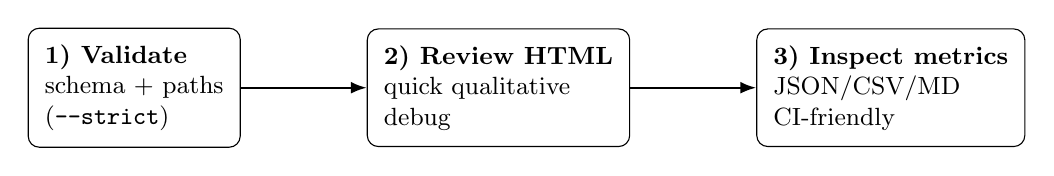
\begin{tikzpicture}[
  node distance=10mm,
  font=\small,
  box/.style={draw, rounded corners, align=left, inner sep=6pt},
  arrow/.style={-{Latex[length=2mm]}, thick}
]

\node[box] (v) {\textbf{1) Validate}\\schema + paths\\(\cmd{--strict})};
\node[box, right=16mm of v] (h) {\textbf{2) Review HTML}\\quick qualitative\\debug};
\node[box, right=16mm of h] (m) {\textbf{3) Inspect metrics}\\JSON/CSV/MD\\CI-friendly};

\draw[arrow] (v) -- (h);
\draw[arrow] (h) -- (m);

\end{tikzpicture}
}
\caption{Recommended result inspection order for fast iteration and reproducible reporting.}
\end{figure}

\begin{enumerate}
  \item \textbf{Validate the schema:}
  \begin{lstlisting}[language=bash]
yolozu validate predictions reports/predict_images.json --strict
  \end{lstlisting}
  \item \textbf{Review the HTML report} to perform rapid qualitative assessments.
  \item \textbf{Inspect the JSON/CSV/MD artifacts} for rigorous quantitative comparisons suitable for CI pipelines and academic publications.
\end{enumerate}

An example workflow for instance segmentation, incorporating HTML and overlay outputs:
\begin{lstlisting}[language=bash]
yolozu eval-instance-seg   --dataset examples/instance_seg_demo/dataset   --split val2017   --predictions examples/instance_seg_demo/predictions/instance_seg_predictions.json   --pred-root examples/instance_seg_demo/predictions   --classes examples/instance_seg_demo/classes.txt   --output reports/instance_seg_eval.json   --html reports/instance_seg_eval.html   --overlays-dir reports/instance_seg_overlays   --max-overlays 10
\end{lstlisting}

\section{Schema validation as a quality gate}
It is imperative to validate prediction artifacts prior to evaluation:
\begin{lstlisting}[language=bash]
python3 tools/validate_predictions.py /path/to/predictions.json --strict
\end{lstlisting}

This practice proactively prevents silent evaluation failures caused by malformed outputs.

\section{Workflow D: Migrate datasets and predictions}
Choose this path when the difficult part is not inference itself, but bridging from an existing dataset or prediction ecosystem into the \yolozu{} interface contract.

YOLOZU provides migration utilities that generate lightweight wrapper artifacts or converters, enabling seamless integration with prevalent ecosystem datasets. The core philosophy is to preserve the original dataset immutability while generating version-controlled wrappers.

\subsection{YOLO-style data.yaml / YOLO (YOLOv8/YOLO11)}
To generate a \path{dataset.json} wrapper from an existing \path{data.yaml}:
\begin{lstlisting}[language=bash]
yolozu migrate dataset   --from auto   --data /path/to/data.yaml   --output data/yolo_wrapper
\end{lstlisting}

Validate the resulting wrapper:
\begin{lstlisting}[language=bash]
yolozu validate dataset data/yolo_wrapper
\end{lstlisting}

\subsection{COCO JSON datasets (YOLOX / Detectron2 / MMDetection)}
To convert COCO instances JSON into YOLO-formatted label text files and generate a corresponding wrapper:
\begin{lstlisting}[language=bash]
yolozu migrate dataset   --from coco   --coco-root /path/to/coco_like_root   --split val2017   --output data/coco_yolo_like   --mode manifest
yolozu validate dataset data/coco_yolo_like --strict
\end{lstlisting}

To export that wrapper into external training layouts:
\begin{lstlisting}[language=bash]
yolozu export-dataset yolo   --dataset data/coco_yolo_like   --split val2017   --out-dir data/coco_yolo_export   --force
yolozu export-dataset coco   --dataset data/coco_yolo_like   --split val2017   --out-dir data/coco_export   --force
yolozu export-dataset kitti   --dataset data/coco_yolo_like   --split val2017   --out-dir data/coco_kitti_export   --force
\end{lstlisting}

For semantic-segmentation descriptors, export keeps the \path{dataset.json} contract while materializing \path{images/} and \path{masks/} into a lightweight external layout:
\begin{lstlisting}[language=bash]
yolozu doctor import --dataset-from auto --dataset /path/to/VOCdevkit/VOC2012 --split val --output -
yolozu import dataset   --from auto   --dataset /path/to/VOCdevkit/VOC2012   --split val   --output reports/voc_seg_wrapper   --force
yolozu export-dataset segmentation   --dataset reports/voc_seg_wrapper   --out-dir reports/voc_seg_export   --image-mode symlink   --force
\end{lstlisting}

For COCO keypoints roots that expose only \path{person_keypoints_<split>.json}, the same auto-detect preflight now recognizes the richer keypoints layout and writes a YOLOZU wrapper with \path{keypoint_names} / \path{skeleton} metadata before export:
\begin{lstlisting}[language=bash]
yolozu doctor import --dataset-from auto --dataset /path/to/coco_keypoints_root --split val2017 --output -
yolozu doctor train-dataset --from coco-keypoints --dataset /path/to/coco_keypoints_root --split val2017 --output -
yolozu import dataset   --from coco-keypoints   --dataset /path/to/coco_keypoints_root   --split val2017   --output reports/coco_keypoints_wrapper   --force
yolozu export-dataset coco   --dataset reports/coco_keypoints_wrapper   --split val2017   --out-dir reports/coco_keypoints_export   --force
\end{lstlisting}

For a repo-bundled tiny sample that exercises automatic detection plus \cmd{COCO -> YOLOZU -> YOLO/COCO/KITTI} end to end:
\begin{lstlisting}[language=bash]
yolozu validate dataset data/conversion_tiny_coco --split val2017 --strict
yolozu doctor import --dataset-from auto --dataset data/conversion_tiny_coco --split val2017 --output -
yolozu migrate dataset   --from auto   --dataset data/conversion_tiny_coco   --split val2017   --output reports/conversion_tiny_wrapper   --force
yolozu export-dataset yolo   --dataset reports/conversion_tiny_wrapper   --split val2017   --out-dir reports/conversion_tiny_yolo   --force
yolozu export-dataset coco   --dataset reports/conversion_tiny_wrapper   --split val2017   --out-dir reports/conversion_tiny_coco   --force
yolozu export-dataset kitti   --dataset reports/conversion_tiny_wrapper   --split val2017   --out-dir reports/conversion_tiny_kitti   --force
\end{lstlisting}

\subsection{Detectron2 / MMDetection predictions interop}
For Detectron2/MMDetection users, keep framework-native inference and only export detections into \path{predictions.json}:
\begin{lstlisting}[language=bash]
python3 tools/export_predictions_detectron2.py   --dataset data/coco_yolo_like   --split val2017   --config /path/to/d2_config.yaml   --weights /path/to/model_final.pth   --protocol nms_applied   --output reports/pred_detectron2.json

python3 tools/export_predictions_mmdet.py   --dataset data/coco_yolo_like   --split val2017   --config /path/to/mmdet_config.py   --checkpoint /path/to/epoch_12.pth   --protocol nms_applied   --output reports/pred_mmdet.json
\end{lstlisting}

Evaluate with explicit class-id normalization to avoid COCO \texttt{category\_id} drift:
\begin{lstlisting}[language=bash]
python3 tools/validate_predictions.py reports/pred_detectron2.json --strict
python3 tools/eval_coco.py   --dataset data/coco_yolo_like   --split val2017   --predictions reports/pred_detectron2.json   --protocol nms_applied   --classes data/coco_yolo_like/labels/val2017/classes.json   --output reports/coco_eval_detectron2.json
\end{lstlisting}

These commands are non-dry by default. Detectron2 requires existing
\cmd{--config} and \cmd{--weights} files; MMDetection requires existing
\cmd{--config} and \cmd{--checkpoint} files. Runtime initialization and
inference for every selected image must complete before a new artifact is
written. Missing prerequisites, unreadable inputs, or runtime/inference errors
return nonzero. Use \cmd{--dry-run} only for schema-valid output that
intentionally skips framework inference.

The exporters record \path{meta.extra.execution_status},
\path{runtime_executed}, and \path{inference_calls}; successful non-dry
artifacts also include config/checkpoint provenance and SHA-256 values in
\path{meta.extra.model_provenance}. Empty detections remain valid after
completed inference. The exporters preserve raw framework box convention
(\cmd{xyxy_abs}) in \path{export_settings.raw_output_bbox_format}, while
normalizing the predictions interface contract output to \cmd{cxcywh_norm} for
strict schema validation.

\subsection{COCO results (inference outputs) \texorpdfstring{$\rightarrow$}{->} predictions.json}
To convert COCO-style detection results into the standardized YOLOZU predictions contract:
\begin{lstlisting}[language=bash]
yolozu migrate predictions   --from coco-results   --results /path/to/coco_results.json   --instances /path/to/instances_val2017.json   --output reports/predictions.json   --force

yolozu validate predictions reports/predictions.json --strict
\end{lstlisting}

\include{chapters/06_calibration_longtail}
\chapter{Tasks: Detection, Segmentation, Keypoints}

\ChapterMeta{
This chapter delineates the supported task families and rigorously defines their expected prediction schemas.
}{
Adhering to these specifications prevents schema mismatches and guarantees the application of the correct evaluator for each task, thereby enhancing metric accuracy and streamlining the debugging process.
}{
It assumes the presence of task-specific data fields (e.g., PNG masks for instance segmentation, and keypoint arrays for pose estimation); it is highly recommended to validate artifacts early using the provided utility tools.
}
\ChapterAudience{Read this chapter when you need to confirm task-specific fields before exporting or evaluating predictions.}


\section{Bounding-box detection}
Bounding-box detection serves as the foundational task, generating per-image detections characterized by class IDs, bounding box coordinates, and confidence scores. Evaluation is predominantly conducted using COCO-style mean Average Precision (mAP) or other protocol-pinned metrics.

\section{Instance segmentation (PNG masks)}
\yolozu{} evaluates instance segmentation utilizing \textbf{per-instance binary PNG masks}. This approach deliberately circumvents the complexities associated with Run-Length Encoding (RLE) or polygon-based tooling.

The minimal required prediction schema is structured as follows:
\begin{lstlisting}[language=json]
[
  {
    "image": "000001.png",
    "instances": [
      {"class_id": 0, "score": 0.9, "mask": "masks/000001_inst0.png"}
    ]
  }
]
\end{lstlisting}

To validate the schema:
\begin{lstlisting}[language=bash]
python3 tools/validate_instance_segmentation_predictions.py   reports/instance_seg_predictions.json
\end{lstlisting}

To execute evaluation and generate visual overlays and HTML reports:
\begin{lstlisting}[language=bash]
python3 tools/eval_instance_segmentation.py   --dataset /path/to/dataset   --split val   --predictions /path/to/predictions.json   --pred-root /path/to/pred-root   --classes /path/to/classes.txt   --html reports/instance_seg_eval.html   --overlays-dir reports/instance_seg_overlays   --max-overlays 10
\end{lstlisting}

\subsection{Real-image TTA compare demo}
For a visible, reproducible compare on real images, \yolozu{} also provides a dedicated instance-seg TTA demo using \texttt{torchvision} Mask R-CNN. It applies a deterministic corruption to a COCO image, runs raw inference, then reruns with augmentation-based TTA. For brightness corruption the demo uses brightness-lift plus horizontal flip; for the other supported corruptions it uses horizontal flip only.
\begin{lstlisting}[language=bash]
yolozu demo instance-seg-tta --run-dir reports/demo_instance_seg_tta
\end{lstlisting}

\noindent Example result from the bundled tiny COCO subset: \path{image\_id=407083},
\path{brightness} severity \path{5}, with \path{tp 2->3}, \path{fp 4->2}, and \path{fn 1->0}.
\noindent Read the figure as follows: green in the delta panel indicates area recovered by TTA or false-positive area removed by TTA; red indicates regression introduced by TTA.

\begin{figure}[h]
  \centering
  \begin{subfigure}[t]{0.32\textwidth}
    \centering
    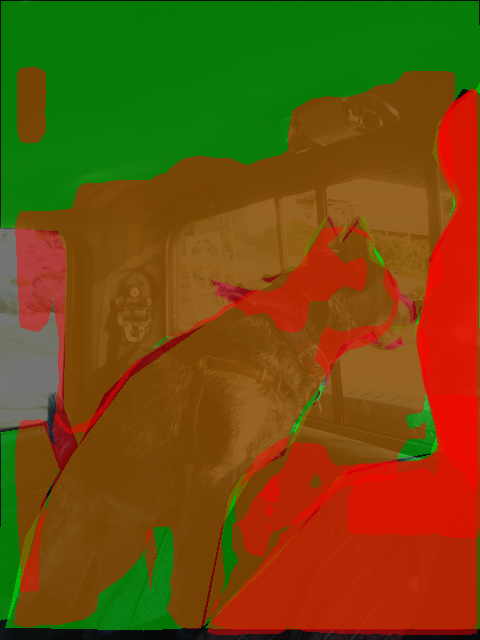
\includegraphics[width=\linewidth]{figures/instance_seg_tta_raw.png}
    \caption{TTA Off}
  \end{subfigure}
  \hfill
  \begin{subfigure}[t]{0.32\textwidth}
    \centering
    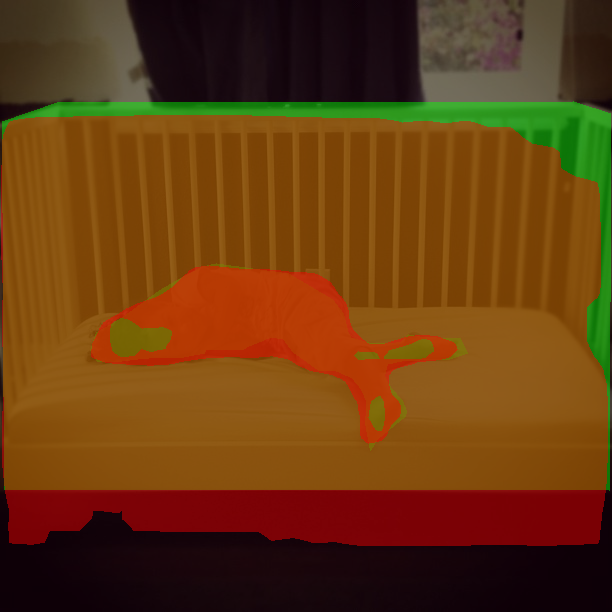
\includegraphics[width=\linewidth]{figures/instance_seg_tta_tta.png}
    \caption{TTA On}
  \end{subfigure}
  \hfill
  \begin{subfigure}[t]{0.32\textwidth}
    \centering
    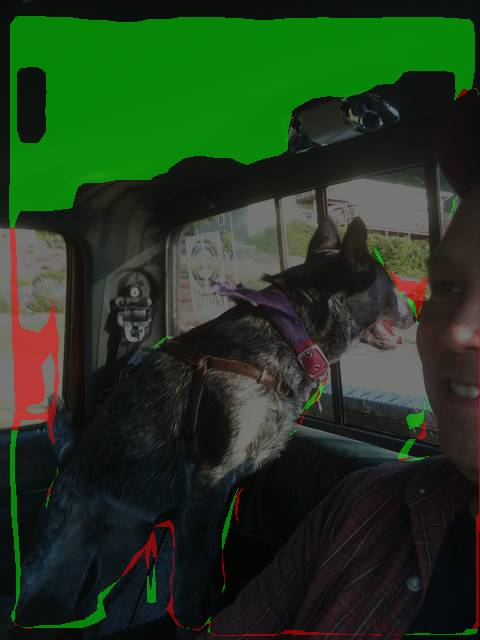
\includegraphics[width=\linewidth]{figures/instance_seg_tta_delta.png}
    \caption{Delta}
  \end{subfigure}
  \caption{Instance segmentation compare on the same corrupted real COCO image. In the Off/On panels, green denotes ground truth and red denotes predicted masks. In the Delta panel, green marks TTA improvements and red marks TTA regressions.}
\end{figure}

\section{Semantic segmentation}
The semantic segmentation suite provides robust dataset preparation utilities and mean Intersection over Union (mIoU) evaluation capabilities. While semantic segmentation evaluation yields mIoU (alongside per-class IoU), instance segmentation evaluation outputs COCO-style mask mAP. Ensure you utilize \path{tools/eval_segmentation.py} for semantic segmentation tasks and \path{tools/eval_instance_segmentation.py} for instance segmentation.

\section{Keypoints / pose estimation}
\yolozu{} fully supports YOLO pose-style keypoints within both labels and predictions, complemented by dedicated evaluation utilities. Depending on your specific workflow requirements, you may employ Percentage of Correct Keypoints (PCK) evaluation, COCO Object Keypoint Similarity (OKS) mAP, or both.

Dataset preparation is streamlined into a single command:
\begin{lstlisting}[language=bash]
python3 tools/yolozu.py prepare-keypoints-dataset   --source /path/to/export   --format auto   --out /path/to/keypoints_dataset
\end{lstlisting}

Supported direct input formats include: \cmd{auto}, \cmd{yolo_pose}, \cmd{coco}, and \cmd{cvat_xml}. When processing CVAT XML, you may provide either a specific XML file or a directory containing an \path{annotations.xml} file. If the image root inference is ambiguous, explicitly define it using the \cmd{--cvat-images-dir} parameter.

A minimal smoke test for CVAT XML processing:
\begin{lstlisting}[language=bash]
python3 -m pytest -q tests/test_prepare_keypoints_dataset_cvat_xml.py
\end{lstlisting}

Keypoint evaluation entry points are accessible via scripts located in the \path{tools/} directory (e.g., keypoint evaluation helpers). Please consult the repository documentation for the authoritative schema definitions and comprehensive usage instructions.

\chapter{Parity, Benchmarks, and Protocols}

\ChapterMeta{
This chapter details parity checking methodologies, protocol-pinned evaluation configurations, and the utilization of benchmark and sweep harnesses.
}{
These tools ensure that comparisons remain stable and actionable by proactively detecting silent numerical drift and systematically tracking performance and metric trends over time.
}{
Execution requires a minimum of two comparable prediction artifacts for parity analysis; protocol-driven runs necessitate pinned settings files alongside consistent preprocessing and output formats.
}

\section{Backend parity}
When exporting predictions across disparate backends (e.g., PyTorch, ONNX Runtime, TensorRT), it is critical to detect any silent numerical drift. Parity tooling systematically compares two prediction artifacts and generates a comprehensive report of any discrepancies.

\begin{figure}[h]
\centering
\resizebox{\linewidth}{!}{%
\begin{tikzpicture}[
  node distance=10mm,
  font=\small,
  box/.style={draw, rounded corners, align=left, inner sep=6pt},
  arrow/.style={-{Latex[length=2mm]}, thick},
  dashedarrow/.style={-{Latex[length=2mm]}, thick, dashed}
]

\node[box] (inputs) {\textbf{Fixed inputs}\\same image subset\\same preprocessing};

\node[box, right=18mm of inputs, yshift=10mm] (a) {\textbf{Backend A}\\torch / onnxrt};
\node[box, right=18mm of inputs, yshift=-10mm] (b) {\textbf{Backend B}\\trt / opencv-dnn};

\node[box, right=20mm of a] (pa) {\path{predictions\_a.json}};
\node[box, right=20mm of b] (pb) {\path{predictions\_b.json}};

\node[box, below=12mm of pb] (par) {\textbf{Parity report}\\diff stats\\(\path{parity.json})};
\node[box, right=20mm of par] (eval) {\textbf{Eval reports}\\metrics JSON\\protocol-pinned};

\draw[dashedarrow] (inputs) -- (a);
\draw[dashedarrow] (inputs) -- (b);
\draw[arrow] (a) -- (pa);
\draw[arrow] (b) -- (pb);
\draw[arrow] (pa) -- (par);
\draw[arrow] (pb) -- (par);
\draw[arrow] (pa) -- (eval);
\draw[arrow] (pb) -- (eval);

\end{tikzpicture}
}
\caption{Apples-to-apples parity: keep inputs fixed, compare exported artifacts, and score with the same evaluator/protocol.}
\end{figure}

\textbf{Conceptual (not copy-paste as-is):} parity command shape.
For a runnable shortest command, use Chapter~5 Workflow A with real artifact paths.
\begin{lstlisting}[language=bash]
yolozu parity   --reference reports/pred_torch.json   --candidate reports/pred_onnxrt.json
\end{lstlisting}

\section{Protocols (pinning evaluation settings)}
Protocols establish immutable evaluation configurations (such as dataset splits, image dimensions, and specific metric keys). This standardization is paramount for ensuring stable, longitudinal comparisons.

For YOLO26 comparisons, the pinned protocol is defined as follows:
\begin{itemize}
  \item Protocol file: \path{protocols/yolo26_eval.json}
  \item Task: \texttt{detect}, Dataset: \texttt{COCO}, Split: \texttt{val2017}
  \item Image size: \texttt{640} (enforcement is the responsibility of the export pipeline)
  \item Bounding box format: \texttt{cxcywh\_norm}
  \item Primary score key: \texttt{map50\_95}
\end{itemize}

A critical semantic rule derived from the protocol documentation:
\begin{itemize}
  \item "End-to-end (e2e) mAP" dictates that the evaluator scores detections exactly as provided; it explicitly does \textit{not} apply Non-Maximum Suppression (NMS).
\end{itemize}

\section{Benchmarks}
Latency and FPS benchmarks constitute a vital component of the regression testing surface.

The recommended user-facing entrypoint is now \cmd{yolozu benchmark}. The
current implementation keeps the honest artifact-first behavior from Phase~1,
and additionally wires real backend orchestration for \cmd{torch},
\cmd{onnx}, and \cmd{engine}. It also accepts \cmd{torchscript} as a
first-class benchmark format, while still recording honest synthetic/skipped
semantics until a dedicated real-orchestration path lands. When the real
backends can execute, the command records a real dataset-pass wall-clock
measurement. When they cannot, it still records skipped formats honestly rather
than fabricating success.

A representative repository-wrapper invocation is:
\begin{lstlisting}[language=bash]
python3 tools/benchmark_model.py \
  --model runs/example/model.pt \
  --onnx-model exports/example.onnx \
  --engine-model exports/example.plan \
  --data data/coco8.yaml \
  --format torch,onnx,engine \
  --protocol nms_applied \
  --latency-source auto \
  --output reports/benchmark_report.json
\end{lstlisting}

The primary artifact set is:
\begin{itemize}
  \item \path{reports/benchmark_report.json}
  \item \path{reports/export_settings_<format>.json}
  \item \path{reports/predictions_<format>.json}
  \item \path{reports/eval_<format>.json}
  \item \path{reports/parity_<format>.json}
\end{itemize}

When \cmd{torch} plus at least one additional real backend (\cmd{onnx} or
\cmd{engine}) complete successfully, \path{parity_<format>.json} is now a real
backend-diff artifact rather than a placeholder. The chosen reference backend
is recorded explicitly (preferring \cmd{torch} when available). Placeholder
parity artifacts remain only for dry-run, skipped, or synthetic-only formats.

\subsection{Gap against the Ultralytics docs surface}
Relative to the public Ultralytics benchmark/export documentation, YOLOZU has
already matched the core benchmark entrypoint shape, but it still trails in
surface breadth.

The most important remaining gaps are:
\begin{itemize}
  \item broader format coverage such as \cmd{openvino}, \cmd{coreml},
  \cmd{saved\_model}, \cmd{tflite}, \cmd{ncnn}, \cmd{rknn}, and \cmd{paddle}
  \item clearer task-specific benchmark expectations for
  \cmd{segmentation}, \cmd{classification}, and \cmd{obb}
  \item stronger validation of format-specific knobs so unsupported
  combinations fail early rather than acting like inert flags
\end{itemize}

This comparison is intentionally about interface behavior and user-facing
surface only. YOLOZU keeps its Apache-2.0-only repository operations policy and
must not pull GPL-licensed implementation code into the repository while
closing these gaps.

For repository-side orchestration, the equivalent wrapper is
\path{tools/benchmark_model.py}.

The benchmark harness, located at \path{tools/benchmark_latency.py}, generates:
\begin{itemize}
  \item A stable JSON report (detailing a single run).
  \item A JSONL history file (facilitating append-only trend tracking).
\end{itemize}

This harness supports both synthetic timing evaluations and configuration-driven, per-bucket executions. In the latter mode, each bucket can ingest externally measured metrics via JSON (for instance, data generated by TensorRT latency measurement scripts).

Typically tracked metrics include FPS and latency quantiles (mean, p50, p90, p95, and p99).

\section{Sweeps}
A sweep harness is indispensable for systematically comparing numerous runs or configurations.

The sweep runner, \path{tools/hpo_sweep.py}, is entirely framework-agnostic and operates by executing templated commands. The core configuration model comprises:
\begin{itemize}
  \item \texttt{base\_cmd}: The command template containing \texttt{\{param\}} placeholders.
  \item \texttt{param\_grid} or \texttt{param\_list}: The defined hyperparameter search space.
  \item Optional keys for metrics extraction and designated output destinations.
\end{itemize}

The default artifacts are designed for effortless diffing and publication:
\path{reports/hpo_sweep.jsonl}, \path{reports/hpo_sweep.csv}, and \path{reports/hpo_sweep.md}.
Utilize the \cmd{--resume} flag to intelligently bypass previously completed parameter combinations.

\chapter{Depth + 6DoF Pose + Symmetry Handling}

\ChapterMeta{
This chapter documents geometry conventions (units, intrinsics, and coordinate frames), pose and translation recovery, and symmetry and commonsense constraint utilities.
}{
It improves correctness and robustness of depth and pose pipelines by making assumptions explicit and by providing reusable postprocess gates.
}{
It requires consistent intrinsics after resize and letterbox, and consistent units; some metrics and utilities require sidecar metadata (for example CAD points) and schema-valid pose fields.
}

\section{Units, intrinsics, and coordinate conventions}
Depth/pose workflows are extremely sensitive to units and to intrinsics consistency.

Key conventions used across docs in this repo:
\begin{itemize}
  \item Intrinsics \cmd{K=(fx,fy,cx,cy)} are in \textbf{pixel units}.
  \item Intrinsics must match the \textbf{image coordinate system used by model outputs} (after resize/letterbox).
  \item Depth \cmd{z} uses the dataset's length unit (YOLOZU does not convert mm\,$\leftrightarrow$\,m).
\end{itemize}

\begin{figure}[h]
\centering
\resizebox{\linewidth}{!}{%
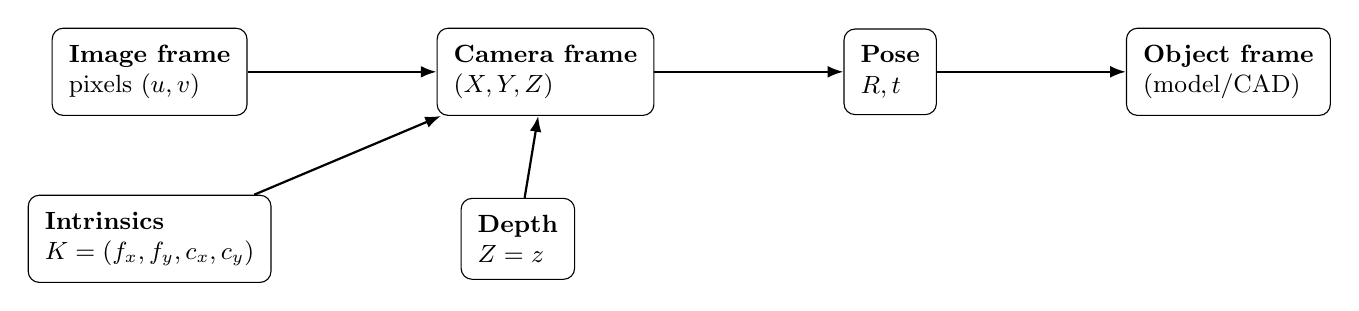
\begin{tikzpicture}[
  node distance=10mm,
  font=\small,
  box/.style={draw, rounded corners, align=left, inner sep=6pt},
  arrow/.style={-{Latex[length=2mm]}, thick}
]

\node[box] (img) {\textbf{Image frame}\\pixels \((u,v)\)};
\node[box, below=10mm of img] (k) {\textbf{Intrinsics}\\\(K=(f_x,f_y,c_x,c_y)\)};
\node[box, right=24mm of k] (z) {\textbf{Depth}\\\(Z=z\)};
\node[box, right=24mm of img] (cam) {\textbf{Camera frame}\\\((X,Y,Z)\)};
\node[box, right=24mm of cam] (pose) {\textbf{Pose}\\\(R,t\)};
\node[box, right=24mm of pose] (obj) {\textbf{Object frame}\\(model/CAD)};

\draw[arrow] (img) -- (cam);
\draw[arrow] (k) -- (cam);
\draw[arrow] (z) -- (cam);
\draw[arrow] (cam) -- (pose);
\draw[arrow] (pose) -- (obj);

\end{tikzpicture}
}
\caption{Coordinate frames: intrinsics and depth connect image pixels to 3D camera coordinates, which are then related to object frame via pose.}
\end{figure}

Depth integration modes in the scaffold trainer:
\begin{itemize}
  \item \cmd{none}: depth disabled (compatibility default).
  \item \cmd{sidecar}: depth is read from sidecar metadata (\cmd{depth_path}/\cmd{depth}) and tracked via \cmd{depth_valid}.
  \item \cmd{fuse_mid}: depth is fused after projector (outside backbone \([P3,P4,P5]\) swap boundary).
\end{itemize}

\begin{figure}[h]
\centering
\resizebox{\linewidth}{!}{%
\begin{tikzpicture}[
  node distance=10mm,
  font=\small,
  box/.style={draw, rounded corners, align=left, inner sep=6pt},
  arrow/.style={-{Latex[length=2mm]}, thick},
  dashedarrow/.style={-{Latex[length=2mm]}, thick, dashed}
]

\node[box] (rgb) {\textbf{RGB image}};
\node[box, below=10mm of rgb] (depth) {\textbf{Depth sidecar} (optional)\\\cmd{depth\_path}/\cmd{depth}};
\node[box, right=20mm of rgb] (pre) {\textbf{Preprocess}\\resize/letterbox\\normalize};
\node[box, right=20mm of pre] (bb) {\textbf{Backbone}\\\([P3,P4,P5]\)};
\node[box, right=20mm of bb] (proj) {\textbf{Projector}\\1x1 convs\\(boundary stable)};
\node[box, right=20mm of proj] (heads) {\textbf{Heads}\\boxes/pose/depth};
\node[box, right=20mm of heads] (pred) {\textbf{Outputs}\\\path{predictions.json}};

\node[box, below=10mm of heads] (fuse) {\textbf{Fuse\_mid} (optional)\\depth fusion\\after projector};

\draw[arrow] (rgb) -- (pre);
\draw[arrow] (pre) -- (bb);
\draw[arrow] (bb) -- (proj);
\draw[arrow] (proj) -- (heads);
\draw[arrow] (heads) -- (pred);

\draw[dashedarrow] (proj) -- (fuse);
\draw[dashedarrow] (fuse) -- (heads);
\draw[dashedarrow] (depth) -- (fuse);

\end{tikzpicture}
}
\caption{Depth modes: \cmd{sidecar} carries depth as metadata; \cmd{fuse\_mid} fuses depth after the projector (outside the backbone swap boundary).}
\end{figure}

Metric safety rule:
\begin{itemize}
  \item Use \cmd{--depth-unit metric} when absolute depth costs are intended.
  \item For \cmd{unspecified}/\cmd{relative}, absolute depth matcher terms are disabled for safety.
\end{itemize}

Example:
\begin{lstlisting}[language=bash]
python3 rtdetr_pose/tools/train_minimal.py \
  --dataset-root data/coco128 \
  --config rtdetr_pose/configs/base.json \
  --use-matcher \
  --depth-mode sidecar \
  --depth-unit metric \
  --depth-scale 1.0
\end{lstlisting}

Practical entry points (``real model'' path):
\begin{itemize}
  \item Training scaffold: \cmd{python3 -m rtdetr_pose.train_minimal ...} (writes metrics and optional run artifacts).
  \item Export predictions: \cmd{python3 tools/export_predictions.py --adapter rtdetr_pose ... --wrap}
  \item No-torch path: use the \cmd{precomputed} adapter with a schema-valid \path{predictions.json}.
\end{itemize}

\section{Typical regression heads}
The 6DoF-oriented design documents and utilities assume per-detection regression heads such as:
\begin{itemize}
  \item \cmd{log_z}: object center depth in log space
  \item \cmd{rot6d}: 6D rotation representation \cite{zhou2019rot6d}
  \item \cmd{offsets}: center correction $(\Delta u,\Delta v)$
  \item \cmd{k_delta}: small intrinsics correction (global / per-frame)
\end{itemize}

See the design spec for clear definitions of frames and outputs:\\
\path{docs/specs/rt_detr_6dof_geom_mim_spec_en_v0_4.md}.

\section{Translation recovery (postprocess)}
A common pattern is to recover translation from depth + intrinsics:
For monocular depth estimation background (if you learn depth from RGB), see \cite{eigen2014depth,ranftl2021dpt}.

Let bbox center be $(u,v)$ and corrected center $(u',v')$ be:
$$
  u' = u + \Delta u, \qquad v' = v + \Delta v.
$$

Let corrected intrinsics be $K'=(f_x', f_y', c_x', c_y')$.
Then with $Z=z$:
$$
  X = \frac{u' - c_x'}{f_x'} Z, \qquad
  Y = \frac{v' - c_y'}{f_y'} Z.
$$

The point of this design is to avoid unstable direct regression of $(X,Y)$.

\section{Commonsense constraints (Stage 4, implemented utilities)}
This repository contains a small, test-covered set of \textbf{commonsense constraints} for depth/pose postprocess.
They are designed as \textbf{utilities} (not a full end-to-end model training system) and can be used both as
train-time regularizers and as inference-time gates/penalties.

Implementation / configuration:
\begin{itemize}
  \item Core logic: \path{yolozu/constraints.py}
  \item Runtime config: \path{configs/runtime/constraints.yaml}
\end{itemize}

Key pieces (matching the Stage 4 roadmap vocabulary):
\begin{itemize}
  \item Depth prior: \\
    \cmd{depth_prior(bbox_wh, size_wh, (fx,fy))} \\
    and penalty \cmd{depth_prior_penalty(z_pred, z_prior)}.
  \item Table plane: signed distance via \cmd{plane_signed_distance(...)}
    and below-plane rejection via \cmd{is_above_plane(...)}.
  \item Upright prior: roll/pitch extraction and violation via \\
    \cmd{upright_violation_deg(R, bounds)}.
\end{itemize}

Wiring example:
\begin{itemize}
  \item Candidate evaluation calls constraints from \path{yolozu/pipeline.py} (\cmd{evaluate_candidate}).
\end{itemize}

Ablations:
\begin{itemize}
  \item Toggle each constraint: \path{tools/ablate_constraints.py}
\end{itemize}

Tests (unit + integration toggles):
\begin{itemize}
  \item \path{tests/test_gates_constraints.py}
  \item \path{tests/test_inference_constraints.py}
\end{itemize}

\section{Handheld camera robustness (Stage 5, implemented utilities)}
Stage 5 focuses on robustness to camera perturbations by consistently using corrected intrinsics $K'$ and
center offsets $(u+\Delta u, v+\Delta v)$.

Implementation entry points:
\begin{itemize}
  \item Intrinsics correction: \path{yolozu/geometry.py} (\cmd{corrected_intrinsics})
  \item Translation recovery using offsets: \path{yolozu/geometry.py} (\cmd{recover_translation})
  \item Jitter profile utilities: \path{yolozu/jitter.py}
\end{itemize}

Jitter utilities provide:
\begin{itemize}
  \item Intrinsics drift sampling (e.g. $\delta f,\delta c$): \cmd{sample\_intrinsics_jitter(...)}
  \item Extrinsics jitter sampling: \cmd{sample\_extrinsics_jitter(...)}
  \item A baseline profile with jitter disabled: \cmd{jitter_off()}
\end{itemize}

Note: the jitter profile includes a \cmd{rolling_shutter} field (\cmd{enabled}, \cmd{line_delay}), but the current
repository code treats it as a configuration stub; there is no physics-accurate rolling shutter model wired into
the core geometry utilities.

Tests (integration-level expectations for jitter on/off profiles):
\begin{itemize}
  \item \path{tests/test_geometry_pipeline.py}
  \item \path{rtdetr_pose/tests/test_train_minimal_sim_jitter.py}
  \item \path{rtdetr_pose/tests/test_train_minimal_extrinsics_jitter.py}
\end{itemize}

\section{Scenario suite (Stage 6, scaffolded validation harness)}
The validation harness includes a lightweight \textbf{scenario suite} that emits a stable JSON report for CI and
tooling integration.

Implementation / schema:
\begin{itemize}
  \item Scenario suite generator: \path{yolozu/scenario_suite.py} (\cmd{build_report})
  \item CLI wrapper: \path{tools/run_scenario_suite.py}
  \item Schema-style stability test: \path{tests/test_scenario_suite.py}
\end{itemize}

Run it manually:
\begin{lstlisting}[language=bash]
python tools/run_scenario_suite.py --output reports/scenario_suite.json
\end{lstlisting}

Important: the current scenario suite produces \textbf{scaffolded/deterministic metrics} (it is a harness and
contract surface), not a substitute for real model evaluation.

\section{Per-detection refinement: Hessian solver}
\yolozu{} includes a Gauss--Newton / Levenberg--Marquardt style refinement utility to iteratively refine
regression head outputs per detection \cite{levenberg1944,marquardt1963lm}.

Key idea: refine per-detection parameters (depth/rotation/offsets) with bounded iterations; treat it as a research postprocess (not a default real-time feature).

\subsection{CLI}
Refine offsets (example):
\begin{lstlisting}[language=bash]
python3 tools/refine_predictions_hessian.py \
  --predictions reports/predictions.json \
  --dataset data/coco128 \
  --output reports/predictions_refined.json \
  --enable \
  --refine-offsets \
  --wrap
\end{lstlisting}

Refine offsets (bounded iterations):
\begin{lstlisting}[language=bash]
python3 tools/refine_predictions_hessian.py \
  --predictions reports/predictions.json \
  --dataset data/coco128 \
  --output reports/predictions_refined.json \
  --enable \
  --refine-offsets \
  --steps 10 \
  --damping 1e-2 \
  --wrap
\end{lstlisting}

\subsection{How it differs from calibration}
\begin{itemize}
  \item Hessian refinement is \textbf{per detection} (local improvements).
  \item L-BFGS calibration is typically \textbf{dataset-wide} (global scale/intrinsics style parameters).
\end{itemize}

Use refinement when you have supervision/constraints and you want to improve individual predictions.
Avoid it for real-time production unless the added latency is justified.

\section{Symmetry: why it matters}
For symmetric objects, a single canonical rotation label may not be unique.
Na\"ively training with a standard rotation loss can be ill-posed and can also break template-based verification.

\section{Symmetry metadata (runtime configuration)}
The preferred approach is deterministic, class-level symmetry metadata.
The runtime config exists at:
\begin{itemize}
  \item \path{configs/runtime/symmetry.json}
\end{itemize}

The expected shape (from the spec) looks like:
\begin{lstlisting}[language=json]
{
  "class_id_or_name": {
    "type": "none | Cn | Dn | Cinf | mirror",
    "n": 4,
    "axis": [0, 0, 1],
    "notes": "optional"
  }
}
\end{lstlisting}

Note: in a fresh checkout, \path{configs/runtime/symmetry.json} may be empty (\cmd{\{\}}). Populate it for your class set.

\section{Symmetry-aware loss / metrics (concept)}
A symmetry-aware rotation distance is commonly expressed as:
$$
  L_{rot}^{sym} = \min_{S \in G} d(R_{pred}, R_{gt} \cdot S)
$$
where $G$ is the symmetry group for the object.

\begin{figure}[h]
\centering
\resizebox{0.95\linewidth}{!}{%
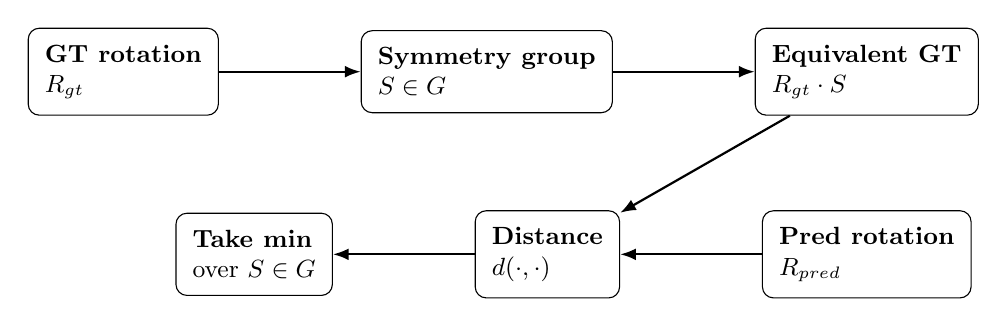
\begin{tikzpicture}[
  node distance=10mm,
  font=\small,
  box/.style={draw, rounded corners, align=left, inner sep=6pt},
  arrow/.style={-{Latex[length=2mm]}, thick}
]

\node[box] (rgt) {\textbf{GT rotation}\\\(R_{gt}\)};
\node[box, right=18mm of rgt] (sym) {\textbf{Symmetry group}\\\(S \in G\)};
\node[box, right=18mm of sym] (eq) {\textbf{Equivalent GT}\\\(R_{gt}\cdot S\)};
\node[box, below=12mm of eq] (rpred) {\textbf{Pred rotation}\\\(R_{pred}\)};
\node[box, left=18mm of rpred] (dist) {\textbf{Distance}\\\(d(\cdot,\cdot)\)};
\node[box, left=18mm of dist] (min) {\textbf{Take min}\\over \(S \in G\)};

\draw[arrow] (rgt) -- (sym);
\draw[arrow] (sym) -- (eq);
\draw[arrow] (eq) -- (dist);
\draw[arrow] (rpred) -- (dist);
\draw[arrow] (dist) -- (min);

\end{tikzpicture}
}
\caption{Symmetry-aware scoring: evaluate rotation error modulo the object's symmetry group.}
\end{figure}

For context and intended gates (including real-time constraints), see:
\begin{itemize}
  \item \path{docs/specs/rt_detr_6dof_geom_mim_spec_en_v0_4.md}
  \item \path{docs/roadmaps/symmetry_commonsense_realtime.md} (historical notes)
\end{itemize}

\section{Available evaluation metrics (current implementation)}
The pose/depth evaluator (\path{yolozu/pose_eval.py}) reports these keys:
\begin{itemize}
  \item Depth: \cmd{depth\_abs_mean}, \cmd{depth\_abs_median}
  \item Pose core: \cmd{rot\_deg_mean}, \cmd{trans\_l2_mean}, \cmd{pose_success}
  \item CAD-point pose: \cmd{add_mean}, \cmd{add_median}, \cmd{adds_mean}, \cmd{adds_median}
\end{itemize}

Definitions:
\begin{itemize}
  \item \textbf{ADD}: mean point distance under fixed point correspondence between $(R_{pred}, t_{pred})$ and $(R_{gt}, t_{gt})$.
  \item \textbf{ADDS}: mean distance from each transformed predicted point to its nearest transformed GT point.
\end{itemize}

These pose metrics and the symmetry caveats around them are discussed in standard 6D pose evaluation literature \cite{hodan2016poseeval,hodan2020bop}.
For an example of a modern end-to-end 6D pose system (useful as conceptual background), see \cite{labbe2020cosypose}.

Input requirements:
\begin{itemize}
  \item Depth metrics require valid GT translation/depth and predicted depth or translation.
  \item ADD/ADDS require CAD points in sidecar metadata \\
    (\cmd{cad_points} / \cmd{cad_path} / \cmd{cad_points_path}) \\
    plus valid GT+pred pose.
\end{itemize}

\section{Practical advice}
\begin{itemize}
  \item First, make unit/intrinsics consistency boring and deterministic.
  \item Next, ensure evaluation metrics treat symmetry correctly for relevant classes.
  \item Keep symmetry/commonsense logic out of the TensorRT graph when possible; run it in postprocess.
\end{itemize}

\chapter{Real-time vs Batch Inference (Research and Deployment)}

\ChapterMeta{
This chapter compares batch and real-time operating modes and outlines the canonical TensorRT pipeline with parity and benchmark safeguards.
}{
It guides you to high-throughput deployment paths while keeping artifact contracts and drift detection in place.
}{
Real-time TensorRT paths are typically Linux with an NVIDIA GPU; parity requires consistent preprocessing and output formats, and expensive extras like TTT and refinement should be explicitly budgeted.
}
\ChapterAudience{Read this chapter when you need to choose between offline throughput and real-time deployment constraints.}


\section{Two operating modes}
\begin{description}
  \item[Batch/offline] Run over a dataset split, export \path{predictions.json}, then evaluate and plot.
  \item[Real-time/streaming] Optimize end-to-end latency and stability; avoid expensive per-frame extras.
\end{description}

\begin{figure}[h]
\centering
\resizebox{\linewidth}{!}{%
\begin{tikzpicture}[
  node distance=10mm,
  font=\small,
  box/.style={draw, rounded corners, align=left, inner sep=6pt},
  arrow/.style={-{Latex[length=2mm]}, thick},
  opt/.style={draw, rounded corners, align=left, inner sep=6pt, dashed}
]

\node[box] (in) {\textbf{Input}\\frame / batch};
\node[box, right=16mm of in] (pre) {\textbf{Preprocess}\\resize/letterbox\\normalize};
\node[opt, right=16mm of pre] (ttt) {\textbf{TTT} (optional)\\bounded-cost};
\node[box, right=16mm of ttt] (eng) {\textbf{Engine}\\torch / onnxrt / trt};
\node[box, right=16mm of eng] (post) {\textbf{Postprocess}\\decode / NMS\\format convert};
\node[opt, right=16mm of post] (ref) {\textbf{Refine / gates} (optional)\\constraints / symmetry};
\node[box, right=16mm of ref] (out) {\textbf{Emit}\\\path{predictions.json}\\+ reports};

\draw[arrow] (in) -- (pre);
\draw[arrow] (pre) -- (ttt);
\draw[arrow] (ttt) -- (eng);
\draw[arrow] (eng) -- (post);
\draw[arrow] (post) -- (ref);
\draw[arrow] (ref) -- (out);

\end{tikzpicture}
}
\caption{Real-time vs batch inference share the same artifact boundary (\cmd{predictions.json}); optional extras must be explicitly budgeted.}
\end{figure}

\section{Non-goals (operational boundaries)}
\begin{itemize}
  \item TTT is \textbf{not} a real-time default. Keep it disabled unless explicitly budgeted and enabled.
  \item If TTT is enabled in streaming mode, use bounded-cost knobs first (e.g., \cmd{--ttt-batch-size 1 --ttt-max-batches 1}).
  \item Hessian refinement is not part of the TensorRT inference graph; treat it as an optional postprocess step.
  \item Real-time claims without hardware-pinned latency/FPS evidence are out of scope for this chapter.
\end{itemize}

\section{Backend choices}
\begin{itemize}
  \item \textbf{Precomputed predictions}: best for integration; works on macOS; use \path{tools/run_scenarios.py} with \cmd{precomputed} adapter.
  \item \textbf{Torch}: flexible for research (TTT, ablations), but slower and less deployable.
  \item \textbf{ONNX Runtime}: CPU-friendly parity reference; useful in CI.
  \item \textbf{TensorRT}: preferred for real-time throughput on Linux+NVIDIA.
\end{itemize}

References:
\begin{itemize}
  \item \path{docs/real_model_interface.md}
  \item \path{docs/tensorrt_pipeline.md}
\end{itemize}

\section{TensorRT pipeline (canonical)}
The typical export route is PyTorch $\rightarrow$ ONNX $\rightarrow$ TensorRT (engine build), with parity checks.

Canonical pattern (artifacts-first):
\begin{itemize}
  \item Export ONNX (+ metadata JSON): \\
    \cmd{python3 tools/export_trt.py} \\
    \cmd{--onnx ...} \cmd{--opset 18} \cmd{--dynamic-hw ...}
  \item Build engine (+ metadata JSON): \\
    \cmd{python3 tools/build_trt_engine.py} \\
    \cmd{--onnx ...} \cmd{--engine ...} \cmd{--precision fp16}
  \item Export \path{predictions.json} from TensorRT and run parity vs ONNXRuntime predictions.
\end{itemize}

The main rule for parity is to keep preprocessing and output formats identical (letterbox/RGB, box format, score scaling), and keep NMS disabled in exported graphs when comparing raw outputs.

\noindent\textbf{Input shape note:} Unlike PyTorch eager mode, ONNXRuntime and TensorRT are typically \textbf{shape-pinned} unless you explicitly export with dynamic axes / optimization profiles. If an ONNX or engine expects (for example) $64\times64$, feeding $640\times640$ will fail. The TensorRT exporter defaults to inferring \cmd{imgsz} from the engine input when possible (and accepts an explicit \cmd{--imgsz} override for dynamic engines).

\section{Stage 7: Performance + deployment safeguards (implemented tooling)}
Stage 7 is about keeping the real-time path fast and predictable.
In this repo, the main safeguards are implemented as \textbf{tooling and contracts} rather than as model-internal graph logic.

\subsection{Keep symmetry/commonsense logic out of TensorRT graphs}
The TensorRT export/build pipeline is designed to focus on the model forward pass.
Symmetry, template scoring, commonsense constraints, and gates are intended to run in \textbf{postprocess} where possible.

\begin{figure}[h]
\centering
\resizebox{0.95\linewidth}{!}{%
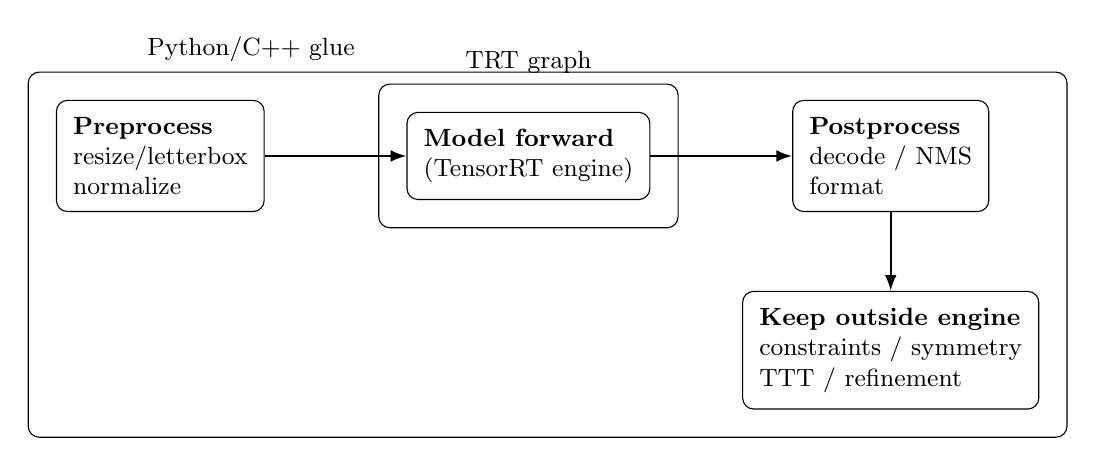
\begin{tikzpicture}[
  node distance=10mm,
  font=\small,
  box/.style={draw, rounded corners, align=left, inner sep=6pt},
  group/.style={draw, rounded corners, inner sep=10pt},
  arrow/.style={-{Latex[length=2mm]}, thick}
]

\node[box] (pre) {\textbf{Preprocess}\\resize/letterbox\\normalize};
\node[box, right=18mm of pre] (fwd) {\textbf{Model forward}\\(TensorRT engine)};
\node[box, right=18mm of fwd] (post) {\textbf{Postprocess}\\decode / NMS\\format};
\node[box, below=10mm of post] (logic) {\textbf{Keep outside engine}\\constraints / symmetry\\TTT / refinement};

\draw[arrow] (pre) -- (fwd);
\draw[arrow] (fwd) -- (post);
\draw[arrow] (post) -- (logic);

\node[group, fit=(fwd), label={[align=left]above:TRT graph}] {};
\node[group, fit=(pre) (post) (logic), label={[align=left]above left:Python/C++ glue}] {};

\end{tikzpicture}
}
\caption{Boundary rule: keep non-forward logic out of the TensorRT graph to simplify deployment and make drift diagnosable.}
\end{figure}

In particular:
\begin{itemize}
  \item Commonsense constraints live in \path{yolozu/constraints.py} and are toggled via \path{configs/runtime/constraints.yaml}.
  \item Parity comparisons are performed on raw outputs (no-NMS exports) so numerical mismatches are detectable.
\end{itemize}

\subsection{Benchmark and regression surfaces}
There are two complementary benchmark surfaces:
\begin{itemize}
  \item A backend-agnostic latency/FPS harness: \path{tools/benchmark_latency.py}
  \item A TensorRT engine latency measurement tool (Linux+NVIDIA + TRT python): \path{tools/measure_trt_latency.py}
\end{itemize}

The harness supports optional targets and can fail the run if targets are not met:
\begin{lstlisting}[language=bash]
python tools/benchmark_latency.py --config configs/benchmark_latency_example.json \
  --target-fps 30
\end{lstlisting}

For a full end-to-end TensorRT run on a Linux+NVIDIA box, use:\\
\path{tools/run_trt_pipeline.py} (export/predictions/parity/eval/latency/benchmark; supports \cmd{--dry-run} for CI-style artifact checks).

\subsection{Gate checks against a baseline}
The repo includes a lightweight gate-check script that compares a current scenario suite report with a saved baseline:
\begin{itemize}
  \item \path{tools/check_gates.py} (writes \path{reports/gate_check.json})
  \item baseline source: \path{reports/baseline.json} (generated by \path{tools/run_baseline.py})
\end{itemize}

The current Stage 7 check is a simple \cmd{fps >= 30} threshold in the gate output.
Note that real FPS validation is inherently \textbf{hardware-dependent}; CI runs can validate the harness and contracts,
while deployment-relevant benchmarks should be run on reference Linux+NVIDIA hardware.

\section{Real-time constraints and optional features}
\subsection{TTT in real-time}
TTT can improve robustness under domain shift but adds latency.
If you use it in streaming mode, keep it bounded:
\begin{itemize}
  \item prefer \cmd{--ttt-preset safe}
  \item start with \cmd{--ttt-batch-size 1 --ttt-max-batches 1}
  \item prefer \cmd{--ttt-reset stream} when you accept cross-image state
\end{itemize}

For controlled comparisons and ablations, use \cmd{--ttt-reset sample} even though it is slower.

\subsection{Per-detection refinement}
Hessian refinement (depth/rotation/offsets) is usually a \textbf{post-inference research tool}.
It is not typically enabled in production unless the added cost is explicitly budgeted.

\section{Batch throughput tips}
\begin{itemize}
  \item Increase batch size first (until memory limits).
  \item Keep dataset subsets deterministic for comparisons.
  \item Record engine metadata (GPU/driver/TensorRT versions) when benchmarking.
\end{itemize}

\section{Mac development vs GPU execution}
If you develop on macOS, keep GPU/TensorRT runs on a Linux+NVIDIA box.
The repo provides a Runpod-oriented path; see \path{deploy/runpod/README.md}.

\subsection{Preflight split for GPU sweep tasks}
Before reserving GPU runtime, generate a local preflight split report:
\begin{lstlisting}[language=bash]
python3 tools/gpu_validation_preflight.py --output reports/gpu_validation_preflight.json
\end{lstlisting}

The report separates:
\begin{itemize}
  \item \path{summary.local_executable_steps}: tasks you can complete locally
  \item \path{summary.gpu_execution_required_steps}: tasks that require Linux+NVIDIA runtime
  \item \path{summary.needs_gpu_runtime_steps}: tasks ready to run once GPU runtime is available
\end{itemize}

Operational runbook: \path{docs/runpod_gpu_validation_split.md}.

When operating via GitHub Actions machine runners instead of RunPod sessions, use
\path{.github/workflows/gpu_zisn_pipeline.yml} (\cmd{workflow_dispatch}) and select
stage \cmd{zisn1}, \cmd{zisn2}, \cmd{zisn3}, or \cmd{all}. The workflow publishes deterministic
DoD summaries to \path{ci-logs/gpu-zisn}.

\section{Inference profiler integration}
The \texttt{yolozu.inference.profiler} module wraps \texttt{torch.profiler} to produce kernel-level latency traces that complement wall-clock benchmarks.

\begin{itemize}
  \item \texttt{profiler\_available()}\\
  checks for \texttt{torch.profiler.profile}.
  \item \texttt{profile\_inference(adapter, records, warmup, active, output\_dir)}\\
  profiles \texttt{adapter.predict()} calls and writes TensorBoard/Chrome-trace output.
  \item \texttt{profile\_callable(fn, *args, iterations, warmup)}\\
  profiles any callable and returns a text summary table.
\end{itemize}

\begin{lstlisting}[language=Python]
from yolozu.inference.profiler import profile_inference, profiler_available

if profiler_available():
    summary = profile_inference(adapter, records, output_dir="runs/profile")
    print(summary)
\end{lstlisting}

\section{torch.compile and ONNX export helpers}
The \texttt{yolozu.inference.torch\_export} module provides two orthogonal utilities:

\begin{itemize}
  \item \texttt{compile\_for\_inference(model, backend, mode)} --- wraps \texttt{torch.compile} with configurable backend (\texttt{inductor}, \texttt{aot\_eager}, etc.) and mode (\texttt{reduce-overhead}, \texttt{max-autotune}). Falls back gracefully when compilation is unavailable.
  \item \texttt{export\_model\_onnx(model, sample\_input, output\_path, opset\_version, ...)} --- exports a \texttt{torch.nn.Module} to ONNX format with configurable opset, dynamic axes, and named I/O.
  \item \texttt{torch\_compile\_available()}, \texttt{torch\_export\_available()} --- feature-detection guards.
\end{itemize}

The \texttt{RTDETRPoseAdapter} integrates \texttt{compile\_for\_inference} via its \texttt{compile\_model}, \texttt{compile\_backend}, and \texttt{compile\_mode} constructor kwargs; when enabled, the model is automatically compiled at first \texttt{predict()} call.

\begin{lstlisting}[language=Python]
from yolozu.inference.torch_export import (
    compile_for_inference, export_model_onnx,
)

fast = compile_for_inference(model, mode="reduce-overhead")
export_model_onnx(model, sample_input, "model.onnx", opset_version=17)
\end{lstlisting}

\section{What to report in papers/notes}
For real-time or deployment-relevant results, always report:
\begin{itemize}
  \item hardware (GPU, driver, CUDA/TensorRT) and engine build settings
  \item end-to-end latency / FPS and measurement method
  \item whether TTT/refinement/gates were enabled and their bounds
\end{itemize}


\part{Training and Research Workflows}
\chapter{Training and the Run Contract}

\ChapterMeta{
This chapter explains the training stack and the run interface contract: stable artifact layout, strict config resolution, and resumable runs.
}{
Following the run interface contract keeps runs reproducible, makes parity checks easier, and keeps outputs predictable across machines and branches.
}{
It assumes run-interface-contract mode, such as \cmd{--run-id} or \cmd{--run-contract}, strict config keys, and the standard training dependencies.
}
\ChapterAudience{Read this chapter when you are running training jobs and want reproducible artifact layout, resume behavior, and tuning surfaces.}

\WorkflowOpening
{Run training so checkpoints, summaries, exports, resume state, and evaluation handoff files land in predictable locations.}
{Use this when YOLOZU owns the reference training run or when an external lane must emit a stable training summary and next-step handoff.}
{A normalized dataset root or wrapper, a YAML/JSON training config, and optional resume/export/parity settings.}
{\cmd{yolozu train ...} for the public route, or \cmd{python3 rtdetr_pose/tools/train_minimal.py ...} when using the low-level reference trainer.}
{\path{runs/<run_id>/checkpoints/}, \path{runs/<run_id>/reports/}, optional \path{exports/}, and \path{training_summary.json}.}
{Check that \path{config_resolved.yaml}, metrics JSONL, checkpoint paths, and optional export/parity reports exist and match the selected run id.}
{Native dataset layouts passed directly to the reference trainer, missing config keys, stale resume paths, backend-specific export failures, or unexpected training dependencies.}

\section{Model-family policy and reference training stack}
YOLOZU interface contracts for predictions, evaluation reports, and scenario outputs are model-family agnostic. The in-repo training reference implementation is the RT-DETR-style adapter under \path{rtdetr_pose/}. The critical part is the \textbf{run interface contract}: stable artifact paths and resumable training runs, independent of the model family that produced them.

\subsection{Dataset-format boundary for the reference trainer}
The RT-DETR reference trainer does not claim that it can ingest every native dataset layout directly at training time. Its expected input is a dataset root that \cmd{build_manifest(...)} can resolve: a YOLO-style root, a YOLO/Ultralytics \path{data.yaml}, or a \path{dataset.json} wrapper with \path{images_dir} and \path{labels_dir} pointing to image files and YOLO label files. The multi-format user convenience layer therefore lives one step earlier: \cmd{yolozu doctor import --dataset-from auto}, \cmd{yolozu import dataset --from auto}, and \cmd{yolozu migrate dataset --from auto} can auto-detect supported native sources such as COCO, COCO keypoints, Ultralytics/YOLO, and the supported semantic-segmentation roots, then materialize a normalized wrapper for training.

In other words, users do not need to manually classify the incoming dataset family, but the reference trainer itself still consumes a train-ready YOLOZU/YOLO-style result of that preflight/import step. Semantic-segmentation descriptors and SynthGen intake shards are import/evaluation inputs unless they are converted into train-ready image and label records. The \cmd{doctor import} report includes \path{reference_trainer.direct_train_ready} and \path{reference_trainer.train_ready_after_migration} so automation can distinguish direct training inputs from native sources that need migration first. The train-specific \cmd{doctor train-dataset} route performs the same check and emits next commands without launching training. It also recognizes explicit \cmd{classification}, \cmd{obb}, \cmd{depth}, and \cmd{pose6d} source families. Classification folders/manifests and OBB labels are recognized intake contracts for external training lanes, not direct RT-DETR reference-trainer inputs. Depth and pose6d are direct only when normalized bbox records include the required sidecars. Through the public CLI, \cmd{python3 -m yolozu train <config> --dataset-root <wrapper>} forwards the dataset root to the RT-DETR reference trainer.

For record-based training, \cmd{python3 -m yolozu train <config> --records-json <train.json> --val-records-json <val.json>} forwards explicit train and validation records to the reference trainer. Both files may be a JSON list of records or an object with an \path{images} list. Records may use either \path{image} or \path{image_path}; label boxes may use flat \path{cx}/\path{cy}/\path{w}/\path{h} fields or nested \path{bbox} fields. OBB records may include \path{angle} or \path{obb}; depth and pose6d records may carry sidecars at the record level or on individual labels. Use this path when the dataset cannot be cleanly represented as one YOLO-style split directory.

\begin{lstlisting}[language=bash]
python3 -m yolozu doctor train-dataset \
  --from auto \
  --dataset /path/to/native_dataset_root \
  --split val2017 \
  --output -
python3 -m yolozu doctor import \
  --dataset-from auto \
  --dataset /path/to/native_dataset_root \
  --split val2017 \
  --output -
python3 -m yolozu migrate dataset \
  --from auto \
  --dataset /path/to/native_dataset_root \
  --split val2017 \
  --output reports/native_dataset_wrapper \
  --force
python3 rtdetr_pose/tools/train_minimal.py \
  --dataset-root reports/native_dataset_wrapper \
  --config rtdetr_pose/configs/base.json \
  --max-steps 50
\end{lstlisting}

COCO keypoints roots can be selected explicitly when needed:
\begin{lstlisting}[language=bash]
python3 -m yolozu doctor train-dataset \
  --from coco-keypoints \
  --dataset /path/to/coco_keypoints_root \
  --split val2017 \
  --output -
python3 -m yolozu import dataset \
  --from coco-keypoints \
  --dataset /path/to/coco_keypoints_root \
  --split val2017 \
  --output reports/coco_keypoints_wrapper \
  --force
\end{lstlisting}

\section{The Run Contract: Rationale and implementation}
A standardized run directory contains:
\begin{itemize}
  \item Checkpoints (e.g., \path{runs/<run-id>/checkpoints/best.pt})
  \item Exported models (e.g., ONNX formats)
  \item Predictions and evaluation reports
  \item Calibration statistics artifacts (when explicitly enabled)
\end{itemize}

This layout makes these operations easier:
\begin{itemize}
  \item Reproducing experiment results
  \item Running parity checks
  \item Comparing runs across Git branches or compute nodes
\end{itemize}

Core rules of the run interface contract, documented here and enforced by the trainer:
\begin{itemize}
  \item Activation via the \cmd{--run-contract} or \cmd{--run-id <id>} flags.
  \item Run-interface-contract mode requires explicit configuration keys and rejects unrecognized keys to prevent silent configuration drift.
  \item A deterministic artifact layout under \path{runs/<run_id>/}:
    \begin{itemize}
      \item \path{checkpoints/last.pt}, \path{checkpoints/best.pt}
      \item \path{reports/train_metrics.jsonl}, \path{reports/val_metrics.jsonl}
      \item \path{reports/config_resolved.yaml}, \path{reports/run_meta.json}, \path{reports/training_summary.json}
    \end{itemize}
  \item Optional export/parity artifacts (when export/parity is enabled):
    \path{exports/model.onnx}, \path{exports/model.onnx.meta.json}, \path{reports/onnx_parity.json}.
  \item Full-state resumption is standardized using the \cmd{--resume} flag, defaulting to \path{runs/<run_id>/checkpoints/last.pt}.
\end{itemize}

\begin{figure}[h]
\centering
\resizebox{\linewidth}{!}{%
\begin{tikzpicture}[
  node distance=10mm,
  font=\small,
  box/.style={draw, rounded corners, align=left, inner sep=6pt},
  arrow/.style={-{Latex[length=2mm]}, thick}
]

\node[box] (root) {\textbf{runs/<run\_id>/}\\stable artifact root};

\node[box, below=14mm of root, xshift=-55mm] (ckpt) {\textbf{checkpoints/}\\\path{last.pt}\\\path{best.pt}};
\node[box, below=14mm of root] (reports) {\textbf{reports/}\\\path{train_metrics.jsonl}\\\path{val_metrics.jsonl}\\\path{config_resolved.yaml}\\\path{run_meta.json}};
\node[box, below=14mm of root, xshift=55mm] (exports) {\textbf{exports/} (optional)\\\path{model.onnx}\\\path{model.onnx.meta.json}};

\node[box, below=12mm of reports] (parity) {\textbf{parity/eval artifacts} (optional)\\\path{reports/onnx_parity.json}\\\path{reports/*.json}};

\draw[arrow] (root) -- (ckpt);
\draw[arrow] (root) -- (reports);
\draw[arrow] (root) -- (exports);
\draw[arrow] (reports) -- (parity);

\end{tikzpicture}
}
\caption{Run directory layout: fixed locations make resume, parity, and cross-branch comparisons reproducible.}
\end{figure}

\subsection{Artifact contract: required vs optional}
\begin{longtable}{@{}p{0.24\textwidth}p{0.26\textwidth}p{0.42\textwidth}@{}}
\toprule
\textbf{Class} & \textbf{Path} & \textbf{Condition} \\
\midrule
Required & \path{runs/<run_id>/checkpoints/last.pt} & Always in contracted runs \\
Required & \path{runs/<run_id>/reports/train_metrics.jsonl} & Always in contracted runs \\
Required & \path{runs/<run_id>/reports/val_metrics.jsonl} & Always in contracted runs \\
Required & \path{runs/<run_id>/reports/config_resolved.yaml} & Always in contracted runs \\
Required & \path{runs/<run_id>/reports/run_meta.json} & Always in contracted runs \\
Optional & \path{runs/<run_id>/exports/model.onnx} & Present when ONNX export is enabled \\
Optional & \path{runs/<run_id>/exports/model.onnx.meta.json} & Present when ONNX export metadata is emitted \\
Optional & \path{runs/<run_id>/reports/onnx_parity.json} & Present when ONNX parity check is executed \\
Optional & \path{runs/<run_id>/reports/training_summary.json} & Present as the backend-neutral top-level summary interface contract \\
\bottomrule
\end{longtable}


\noindent\textbf{Note (low-level trainer):} When invoking \cmd{python3 -m rtdetr_pose.train_minimal} directly, specifying \cmd{--run-id} implicitly activates run-contract mode and necessitates a \cmd{--config} argument (a YAML/JSON file such as \path{configs/examples/train_contract.yaml}). For rapid smoke tests bypassing the run contract, use explicit values such as \cmd{--run-dir runs/exp001} and \cmd{--onnx-out runs/exp001/model.onnx}.

\section{Configuration resolution and strictness}
The training entry point reads YAML/JSON configurations via \cmd{--config}, then applies explicit CLI overrides. The resolution hierarchy is:
\begin{center}
\textbf{CLI flags \(>\) config file \(>\) built-in defaults}
\end{center}

Configuration keys must correspond exactly to their argparse destination names (e.g., \cmd{--weight-decay} maps to \texttt{weight\_decay}). In run-contract mode (triggered by \texttt{run\_contract} or \texttt{run\_id}), any unrecognized keys are immediately rejected, thereby eliminating the risk of silent configuration drift.

\begin{figure}[h]
\centering
\resizebox{0.95\linewidth}{!}{%
\begin{tikzpicture}[
  node distance=10mm,
  font=\small,
  box/.style={draw, rounded corners, align=left, inner sep=6pt},
  arrow/.style={-{Latex[length=2mm]}, thick}
]

\node[box] (cli) {\textbf{CLI flags}\\explicit overrides\\(\cmd{--lr}, \cmd{--amp}, ...)};
\node[box, below=10mm of cli] (cfg) {\textbf{Config file}\\YAML/JSON via \cmd{--config}};
\node[box, below=10mm of cfg] (def) {\textbf{Built-in defaults}\\conservative baseline};

\node[box, right=28mm of cfg] (resolved) {\textbf{Resolved config}\\\path{config_resolved.yaml}\\(run artifact)};
\node[box, right=28mm of resolved] (strict) {\textbf{Strict mode}\\unknown keys fail\\(no silent drift)};

\draw[arrow] (cli) -- (resolved);
\draw[arrow] (cfg) -- (resolved);
\draw[arrow] (def) -- (resolved);
\draw[arrow] (resolved) -- (strict);

\end{tikzpicture}
}
\caption{Configuration resolution: the run contract enforces explicit keys and produces a resolved config artifact.}
\end{figure}

\section{YAML workflows: train / resume / test}
A unified project structure supports YAML-driven execution for both training and testing scenarios.

\begin{longtable}{@{}p{0.18\textwidth}p{0.30\textwidth}p{0.46\textwidth}@{}}
\toprule
\textbf{Workflow} & \textbf{Primary config} & \textbf{Reference command} \\
\midrule
Train (starter config) & \path{configs/examples/train_setting.yaml} & \cmd{yolozu train <train_setting.yaml>} \\
Train (run contract) & \path{configs/examples/train_contract.yaml} & \cmd{yolozu train <train_contract.yaml> --run-id <id>} \\
Resume (full state) & Same as contract & \cmd{yolozu train <train_contract.yaml> --run-id <id> --resume} \\
Test (scenario runner) & \path{configs/examples/test_setting.yaml} & \cmd{yolozu test <test_setting.yaml> [test_args...]} \\
\bottomrule
\end{longtable}

Example execution commands:
\begin{lstlisting}[language=bash]
yolozu train configs/examples/train_setting.yaml
yolozu train configs/examples/train_contract.yaml --run-id exp01
yolozu train configs/examples/train_contract.yaml --run-id exp01 --resume
yolozu test configs/examples/test_setting.yaml --adapter precomputed --predictions reports/predictions.json
\end{lstlisting}


\noindent For \cmd{yolozu test}, YAML keys are dynamically translated into \cmd{--key value} arguments (with booleans converted to flags), allowing subsequent CLI arguments to override them as necessary.

\section{Backend interface and orchestration}
The training platform now separates five concerns:
\begin{enumerate}
  \item a canonical \cmd{TrainConfig} projection,
  \item a backend registry,
  \item a shared \path{training_summary.json} style interface contract,
  \item a capability matrix, and
  \item a lightweight orchestration entrypoint.
\end{enumerate}

This means the reference trainer and the external lanes do not need to share
one internal loop, but they do share one top-level description of what ran and
what artifacts were promised.

For external lanes, YOLOZU now also standardizes one wrapper-level bundle under
\path{work_dir/}:
\begin{itemize}
  \item \path{dataset/}
  \item \path{configs/train_config_projection.json}
  \item \path{reports/training_summary.json}
  \item \path{reports/external_run_meta.json}
  \item \path{reports/launcher_plan.json}
  \item \path{reports/execution.json}
  \item \path{reports/resume_handoff.json}
  \item \path{reports/export_handoff.json}
  \item \path{reports/eval_handoff.json}
  \item \path{reports/parity_handoff.json}
  \item \path{reports/training_registry_entry.json}
\end{itemize}

This is not the same as forcing one backend-native checkpoint layout. It means
the wrapper-owned interface contract is now fixed even when the actual trainer
remains external.

The external training summary also records \path{next_steps}: copy-paste
follow-up commands for resume, export, evaluation, and parity. The handoff JSONs make
those next steps machine-readable, so orchestration and CI do not need to infer
backend-specific conventions from prose. In practice, this makes the training
report itself the hand-off note for the next operator step while still keeping
the resume/export/eval/parity interface contract explicit.

OpenCV DNN and ONNX Runtime do not appear in this training registry because
YOLOZU treats them as inference/export runtimes after training, not as
training backends in their own right.

The repo-side orchestration command is:
\begin{lstlisting}[language=bash]
yolozu train-orchestrate \
  --spec reports/train_orchestration_spec.json \
  --output reports/training_orchestration_report.json \
  --registry-out reports/training_registry.jsonl
\end{lstlisting}

When \cmd{--registry-out} is set, each executed training run appends one
\path{yolozu_training_registry_entry_v1} record to a shared JSONL file.
This is intentionally lightweight: it is an append-only experiment registry for
cross-backend auditing, not a full experiment tracking server.

Read next:
\begin{itemize}
  \item \path{docs/training_backend_interface.md}
  \item \path{docs/training_capability_matrix.md}
  \item \path{docs/training_orchestration.md}
\end{itemize}

\section{External framework finetune smoke matrix}
For user convenience, YOLOZU includes template configs and a unified smoke runner for external finetune entrypoints:
\begin{itemize}
  \item YOLO-family runtime
  \item Detectron2
  \item MMDetection
  \item MMPose
  \item MMSeg
  \item NVIDIA TAO
  \item RT-DETR (\path{rtdetr_pose})
\end{itemize}

Template paths:
\begin{itemize}
  \item \path{configs/examples/finetune_external/yolo_runtime_yolov8n_finetune_smoke.yaml}
  \item \path{configs/examples/finetune_external/mmdetection_finetune_smoke.py}
  \item \path{configs/examples/finetune_external/mmpose_finetune_smoke.py}
  \item \path{configs/examples/finetune_external/mmseg_finetune_smoke.py}
  \item \path{configs/examples/finetune_external/tao_finetune_smoke.yaml}
  \item \path{configs/examples/finetune_external/detectron2_finetune_smoke.yaml}
  \item \path{configs/examples/finetune_external/rtdetr_pose_finetune_smoke.yaml}
\end{itemize}

Unified smoke command (interface contract report):
\begin{lstlisting}[language=bash]
python3 tools/run_external_finetune_smoke.py \
  --dataset-root data/smoke \
  --split train \
  --output reports/external_finetune_smoke.json
\end{lstlisting}

Top-level Detectron2 training lane examples:
\begin{lstlisting}[language=bash]
python3 -m yolozu train \
  --external-backend detectron2 \
  configs/examples/finetune_external/detectron2_finetune_smoke.yaml \
  --dataset data/smoke \
  --split val \
  --task-family bbox \
  --dry-run \
  --output reports/train_external_detectron2_bbox.json

python3 -m yolozu train \
  --external-backend detectron2 \
  /path/to/mask_rcnn_config.yaml \
  --dataset /path/to/dataset \
  --split train \
  --task-family segmentation \
  --train-opt DATASETS.TRAIN "(\"my_seg_train\",)" \
  --dry-run \
  --output reports/train_external_detectron2_seg.json

python3 -m yolozu train \
  --external-backend detectron2 \
  /path/to/keypoint_rcnn_config.yaml \
  --dataset /path/to/dataset \
  --split train \
  --task-family keypoints \
  --train-opt DATASETS.TRAIN "(\"my_kpts_train\",)" \
  --dry-run \
  --output reports/train_external_detectron2_keypoints.json
\end{lstlisting}

Execute real training for selected frameworks:
\begin{lstlisting}[language=bash]
python3 tools/run_external_finetune_smoke.py \
  --dataset-root data/smoke \
  --split train \
  --non-dry-framework yolov \
  --non-dry-framework rtdetr \
  --epochs 1 --max-steps 1 --batch-size 2 --image-size 96 \
  --device cpu \
  --require-training-execution \
  --output reports/external_finetune_smoke.exec.json
\end{lstlisting}

MMDetection/Detectron2 can be wired to external launchers via
\cmd{--mmdet-train-script} and \cmd{--detectron2-train-script}.
RT-DETR non-dry dependency failures are explicit in the report
(\texttt{failure\_code=E\_DEP\_TORCH\_MISSING}).
When MMDetection/Detectron2 projection dependencies are absent, train-path audit can still continue with external launchers; the report records \texttt{projection\_error} and \texttt{train\_path\_audited}.

GPU check (machine.dev style) example:
\begin{lstlisting}[language=bash]
python3 tools/run_external_finetune_smoke.py \
  --dataset-root data/smoke \
  --split train \
  --non-dry-framework rtdetr \
  --device cuda \
  --epochs 1 --max-steps 1 --batch-size 2 --image-size 96 \
  --require-training-execution \
  --output reports/external_finetune_smoke.machine_dev.json
\end{lstlisting}

\section{Solver (optimizer) parameters and defaults}
The supported optimizers are \texttt{adamw} (the default) and \texttt{sgd}.

\begin{longtable}{@{}p{0.40\textwidth}p{0.10\textwidth}p{0.12\textwidth}p{0.30\textwidth}@{}}
\toprule
\textbf{CLI / config key} & \textbf{Type} & \textbf{Default} & \textbf{Notes} \\
\midrule
\cmd{--optimizer} / \texttt{optimizer} & str & \texttt{adamw} & \texttt{adamw}, \texttt{sgd} \\
\cmd{--lr} / \texttt{lr} & float & \texttt{1e-4} & Base learning rate \\
\cmd{--weight-decay} / \texttt{weight\_decay} & float & \texttt{0.01} & Base weight decay \\
\cmd{--momentum} / \texttt{momentum} & float & \texttt{0.9} & Applicable to SGD only \\
\cmd{--nesterov} / \texttt{nesterov} & bool & \texttt{false} & Applicable to SGD only \\
\cmd{--use-param-groups} / \texttt{use\_param\_groups} & bool & \texttt{false} & Enables separate backbone/head parameter groups \\
\cmd{--backbone-lr-mult} / \texttt{backbone\_lr\_mult} & float & \texttt{1.0} & Learning rate multiplier for the backbone \\
\cmd{--head-lr-mult} / \texttt{head\_lr\_mult} & float & \texttt{1.0} & Learning rate multiplier for the head \\
\cmd{--backbone-wd-mult} / \texttt{backbone\_wd\_mult} & float & \texttt{1.0} & Weight decay multiplier for the backbone \\
\cmd{--head-wd-mult} / \texttt{head\_wd\_mult} & float & \texttt{1.0} & Weight decay multiplier for the head \\
\cmd{--wd-exclude-bias} / \texttt{wd\_exclude\_bias} & bool & \texttt{true} & Sets bias decay to 0 \\
\cmd{--wd-exclude-norm} / \texttt{wd\_exclude\_norm} & bool & \texttt{true} & Sets normalization decay to 0 \\
\bottomrule
\end{longtable}

\section{LR scheduling parameters and defaults}
Supported learning rate scheduler configurations include \texttt{none} (default), \texttt{cosine}, \texttt{onecycle}, and \texttt{multistep}.

\begin{longtable}{@{}p{0.40\textwidth}p{0.10\textwidth}p{0.12\textwidth}p{0.30\textwidth}@{}}
\toprule
\textbf{CLI / config key} & \textbf{Type} & \textbf{Default} & \textbf{Notes} \\
\midrule
\cmd{--scheduler} / \texttt{scheduler} & str & \texttt{none} & \texttt{none}, \texttt{cosine}, \texttt{onecycle}, \texttt{multistep} \\
\cmd{--min-lr} / \texttt{min\_lr} & float & \texttt{0.0} & Corresponds to cosine \texttt{eta\_min} \\
\cmd{--scheduler-milestones} / \texttt{scheduler\_milestones} & str/list & \texttt{""} & Comma-separated list for multistep scheduling \\
\cmd{--scheduler-gamma} / \texttt{scheduler\_gamma} & float & \texttt{0.1} & Decay factor for multistep scheduling \\
\cmd{--lr-warmup-steps} / \texttt{lr\_warmup\_steps} & int & \texttt{0} & Number of linear warmup steps \\
\cmd{--lr-warmup-init} / \texttt{lr\_warmup\_init} & float & \texttt{0.0} & Initial learning rate during warmup \\
\bottomrule
\end{longtable}


\noindent\textbf{Note:} The \texttt{linear} scheduler is not supported in the current codebase.

\section{LoRA / QLoRA parameters and defaults}
Low-Rank Adaptation (LoRA) is activated when \texttt{lora\_r > 0}.
For the plain-language intuition and the difference between LoRA and QLoRA, see Chapter~14 before tuning these knobs.

\paragraph{What these words mean in plain language.}
\begin{itemize}
  \item \textbf{LoRA} stands for \textbf{Low-Rank Adaptation}. Instead of updating every weight in a large model, LoRA adds a small trainable adapter on top of selected layers. In practice, this means ``keep most of the base model fixed, and learn a compact correction.''
  \item \textbf{Why people use LoRA}: it reduces memory cost, usually trains faster than full-model finetuning, and makes it easier to keep one base checkpoint while testing several small adaptation variants.
  \item \textbf{\texttt{lora\_r}} is the adapter rank. A larger rank means a more expressive adapter, but also more trainable parameters.
  \item \textbf{\texttt{lora\_alpha}} is a scaling factor for the adapter contribution. A simple mental model is: rank controls adapter capacity, alpha controls how strongly the adapter is allowed to matter.
  \item \textbf{QLoRA} means ``LoRA on top of a quantized base model.'' In this repository, \texttt{--qlora} keeps the trainable LoRA adapters, but stores the frozen base model in a lower-precision quantized form to reduce memory further.
  \item \textbf{Why QLoRA is stricter}: because quantization and adapter training interact. That is why \yolozu{} enforces the safe combination explicitly instead of pretending every LoRA run is also a safe QLoRA run.
\end{itemize}

\paragraph{A simple comparison.}
\begin{itemize}
  \item \textbf{Full finetuning}: move almost every parameter.
  \item \textbf{LoRA finetuning}: keep the base model mostly fixed and train small adapters.
  \item \textbf{QLoRA finetuning}: same adapter idea as LoRA, but the frozen base model is additionally quantized to save memory.
\end{itemize}

\begin{longtable}{@{}p{0.40\textwidth}p{0.10\textwidth}p{0.12\textwidth}p{0.30\textwidth}@{}}
\toprule
\textbf{CLI / config key} & \textbf{Type} & \textbf{Default} & \textbf{Notes} \\
\midrule
\cmd{--lora-r} / \texttt{lora\_r} & int & \texttt{0} & Values \texttt{>0} enable LoRA \\
\cmd{--lora-alpha} / \texttt{lora\_alpha} & float/null & \texttt{null} & A null value implies \(\alpha=r\) \\
\cmd{--lora-dropout} / \texttt{lora\_dropout} & float & \texttt{0.0} & Specifies LoRA input dropout \\
\cmd{--lora-target} / \texttt{lora\_target} & str & \texttt{head} & Options: \texttt{head}, \texttt{all\_linear}, \texttt{all\_conv1x1}, \texttt{all\_linear\_conv1x1} \\
\cmd{--lora-freeze-base} / \texttt{lora\_freeze\_base} & bool & \texttt{true} & Restricts training exclusively to LoRA parameters \\
\cmd{--lora-train-bias} / \texttt{lora\_train\_bias} & str & \texttt{none} & Options: \texttt{none}, \texttt{all} \\
\cmd{--torchao-quant} / \texttt{torchao\_quant} & str & \texttt{none} & Options: \texttt{none}, \texttt{int8wo}, \texttt{int4wo} \\
\cmd{--torchao-required} / \texttt{torchao\_required} & bool & \texttt{false} & Triggers a failure if the quantization backend is absent \\
\cmd{--qlora} / \texttt{qlora} & bool & \texttt{false} & Requires LoRA; strictly enforces int4wo quantization and base freezing \\
\bottomrule
\end{longtable}

\section{Default configuration list (practical minimum)}
The canonical default configurations are maintained within:
\begin{itemize}
  \item \path{configs/examples/train_setting.yaml}
  \item \path{configs/examples/train_contract.yaml}
  \item \path{configs/examples/test_setting.yaml}
\end{itemize}

Frequently modified default parameters include:
\begin{longtable}{@{}p{0.34\textwidth}p{0.20\textwidth}p{0.40\textwidth}@{}}
\toprule
\textbf{Config key} & \textbf{Default} & \textbf{Meaning} \\
\midrule
\texttt{optimizer} & \texttt{adamw} & Optimizer family \\
\texttt{lr} & \texttt{1e-4} & Base learning rate \\
\texttt{weight\_decay} & \texttt{0.01} & Base weight decay \\
\texttt{scheduler} & \texttt{none} & Learning rate scheduler mode \\
\texttt{lr\_warmup\_steps} & \texttt{0} & Warmup is disabled by default \\
\texttt{lora\_r} & \texttt{0} & LoRA is disabled by default \\
\texttt{gradient\_accumulation\_steps} & \texttt{1} & Gradient accumulation is disabled \\
\texttt{clip\_grad\_norm} & \texttt{0.0} & Gradient clipping is disabled \\
\texttt{use\_ema} & \texttt{false} & Exponential Moving Average (EMA) is disabled \\
\texttt{amp} & \texttt{none} & Automatic Mixed Precision (AMP) is disabled \\
\texttt{metrics\_jsonl} & \path{reports/train_metrics.jsonl} & Output stream for training metrics \\
\texttt{metrics\_csv} & \path{reports/train_metrics.csv} & Tabular format for metrics \\
\texttt{export\_onnx} & \texttt{true} & ONNX export is enabled \\
\texttt{onnx\_out} & \path{reports/rtdetr_pose.onnx} & Designated ONNX output path \\
\bottomrule
\end{longtable}

\section{Smoke training}
For a repository-wide offline smoke, use:
\begin{lstlisting}[language=bash]
bash scripts/smoke.sh
\end{lstlisting}

For training-entrypoint coverage across external frameworks, use the dedicated
interface-contract smoke runner:
\begin{lstlisting}[language=bash]
python3 tools/run_external_finetune_smoke.py \
  --dataset-root data/smoke \
  --split train \
  --output reports/external_finetune_smoke.json
\end{lstlisting}

The first command exercises the main offline smoke lane. The second focuses on
finetune-entrypoint audit for YOLOv/MMDetection/Detectron2/RT-DETR style
training surfaces and writes a machine-readable report.

\section{Depth mode in training (current implementation)}
The in-repo RT-DETR Pose trainer incorporates optional depth integration, configured with a conservative default:
\begin{itemize}
  \item \cmd{--depth-mode none} (default): Executes the baseline pathway with depth processing disabled.
  \item \cmd{--depth-mode sidecar}: Ingests per-image depth sidecars (\cmd{depth_path}/\cmd{depth}) and propagates the \cmd{depth_valid} flag.
  \item \cmd{--depth-mode fuse_mid}: Implements lightweight depth fusion subsequent to the projector (external to the backbone boundary).
\end{itemize}

Safety controls:
\begin{itemize}
  \item \cmd{--depth-unit \{unspecified,relative,metric\}} (default: \cmd{unspecified}).
  \item Absolute depth matcher costs are strictly permitted only in metric mode; non-metric modes automatically disable \cmd{cost_z}/\cmd{cost_t} for safety.
  \item \cmd{--depth-scale} applies a scalar multiplier to sidecar depth values.
  \item \cmd{--depth-dropout} regulates the modality dropout probability during \cmd{fuse_mid} training.
\end{itemize}

\section{Contracted run example}
\begin{lstlisting}[language=bash]
yolozu train configs/examples/train_contract.yaml --run-id exp01

# Resume training from runs/exp01/checkpoints/last.pt
yolozu train configs/examples/train_contract.yaml --run-id exp01 --resume
\end{lstlisting}

\section{Backbone modification (adapter-scoped architecture switch)}
Backbone-specific configurations are not primarily governed by solver flags; rather, they are derived from the model configuration file specified by \texttt{model\_config} in the training YAML.
This section applies to the in-repo \path{rtdetr_pose} adapter boundary.

Backbone notes and examples are maintained in \path{docs/backbones.md}.

The backbone output contract strictly mandates three feature maps: \texttt{[P3, P4, P5]} with corresponding strides of \texttt{[8, 16, 32]}. Each level is independently projected to the transformer's \texttt{d\_model} dimension via 1x1 convolutions, then processed by the RT-DETR-style FPN/PAN + hybrid encoder path.

Supported backbone architectures in the current codebase include:
\texttt{cspresnet}, \texttt{tiny\_cnn}, \texttt{cspdarknet\_s}, \texttt{resnet50}, and \texttt{convnext\_tiny}.

While legacy compatibility fields (e.g., \texttt{backbone\_name}, \texttt{backbone\_channels}) remain functional, the strongly preferred convention is to use \path{model.backbone.*} together with \path{model.projector.d_model}.

\begin{longtable}{@{}p{0.28\textwidth}p{0.24\textwidth}p{0.42\textwidth}@{}}
\toprule
\textbf{Location} & \textbf{Key} & \textbf{Role} \\
\midrule
Train YAML & \texttt{model\_config} & References the model JSON (e.g., \path{rtdetr_pose/configs/base.json}) \\
Model JSON (\texttt{model.backbone.*}) & \texttt{name} & Specifies the backbone family (e.g., \texttt{cspresnet}, \texttt{cspdarknet\_s}, \texttt{resnet50}, \texttt{convnext\_tiny}) \\
Model JSON (\texttt{model.backbone.*}) & \texttt{norm} & Defines the normalization type (\texttt{bn|syncbn|frozenbn|gn}) \\
Model JSON (\texttt{model.backbone.*}) & \texttt{args} & Optional, backbone-specific constructor arguments \\
Model JSON (\texttt{model.projector.*}) & \texttt{d\_model} & Sets the projection/output channel size for transformer input \\
Solver YAML/CLI & \texttt{backbone\_lr\_mult} & Learning rate multiplier applied to backbone parameters \\
Solver YAML/CLI & \texttt{backbone\_wd\_mult} & Weight decay multiplier applied to backbone parameters \\
\bottomrule
\end{longtable}

Normalization guidelines:
\begin{itemize}
  \item \texttt{bn}: The standard default for single-node training.
  \item \texttt{syncbn}: Highly recommended for multi-GPU environments utilizing small per-rank batch sizes.
  \item \texttt{frozenbn}: Provides stability when batch statistics must remain static.
  \item \texttt{gn}: A robust, batch-size-independent alternative.
\end{itemize}

Recommended workflow for backbone modification:
\begin{enumerate}
  \item Duplicate \path{rtdetr_pose/configs/base.json} to create a project-local model JSON file.
  \item Modify \texttt{model.backbone.name} and \texttt{model.backbone.args} as required.
  \item Configure \texttt{model.projector.d\_model} to match the intended transformer hidden size.
  \item Update the training YAML's \texttt{model\_config} to reference the newly created JSON file.
  \item Initiate a smoke test with minimal settings (e.g., reduced \texttt{image\_size} and \texttt{max\_steps}) before scaling up.
\end{enumerate}

Example implementation:
\begin{lstlisting}[language=bash]
cp rtdetr_pose/configs/base.json rtdetr_pose/configs/my_backbone.json
# Edit model.backbone.name, model.backbone.args, and model.projector.d_model accordingly

yolozu train configs/examples/train_setting.yaml   --model-config rtdetr_pose/configs/my_backbone.json   --use-param-groups   --backbone-lr-mult 0.1
\end{lstlisting}

\section{PyTorch utility wrappers}
The \texttt{yolozu.training.torch\_utils} module provides thin wrappers around core PyTorch APIs for common training and inference tasks:

\begin{itemize}
  \item \texttt{amp\_inference\_context()} --- wraps \texttt{torch.amp.autocast} for mixed-precision inference.
  \item \texttt{compile\_model()} --- wraps \texttt{torch.compile} with configurable backend/mode.
  \item \texttt{profile\_callable()} --- wraps \texttt{torch.profiler} and returns structured event summaries.
  \item \texttt{model\_info()} --- reports parameter counts, dtype breakdown, device, and buffer stats.
  \item \texttt{auto\_device()} --- auto-detects the best available device (CUDA $\to$ MPS $\to$ CPU).
  \item \texttt{seed\_everything()} --- sets all random seeds (Python, NumPy, PyTorch) for reproducibility.
\end{itemize}

\begin{lstlisting}[language=Python]
from yolozu.training.torch_utils import (
    amp_inference_context, compile_model, model_info,
    auto_device, seed_everything,
)

seed_everything(42)
device = auto_device()
model = model.to(device)
compiled = compile_model(model, mode="reduce-overhead")
print(model_info(compiled))

with amp_inference_context(device.type):
    output = compiled(images)
\end{lstlisting}

\section{AMP utilities for training loops}
The \texttt{yolozu.training.amp\_utils} module provides a thin wrapper around \texttt{torch.amp} that standardizes Automatic Mixed Precision setup across SDFT distillation, TTA/TTT loops, and custom training scripts.

\begin{itemize}
  \item \texttt{amp\_available()} --- returns \texttt{True} when \texttt{torch.amp.autocast} is present (PyTorch 2.x).
  \item \texttt{make\_amp\_context(device\_type, dtype, enabled)} --- creates a paired \texttt{(autocast\_factory, GradScaler|None)} tuple. A \texttt{GradScaler} is only returned for \texttt{float16} on CUDA; for \texttt{bfloat16}, MPS, or CPU the scaler is \texttt{None}.
\end{itemize}

\begin{lstlisting}[language=Python]
from yolozu.training.amp_utils import make_amp_context

autocast_ctx, scaler = make_amp_context(device_type="cuda", dtype="float16")
with autocast_ctx():
    loss = model(inputs)
if scaler is not None:
    scaler.scale(loss).backward()
    scaler.step(optimizer)
    scaler.update()
else:
    loss.backward()
    optimizer.step()
\end{lstlisting}

\section{Torchvision v2 transforms bridge}
The \texttt{yolozu.training.transforms\_bridge} module provides composable augmentation pipelines using \texttt{torchvision.transforms.v2} (stable since torchvision 0.17). These pipelines jointly transform images, bounding boxes, and keypoints in a single call.

\begin{itemize}
  \item \texttt{transforms\_v2\_available()} --- checks whether \texttt{torchvision.transforms.v2} is importable.
  \item \texttt{build\_detection\_transforms(size, hflip\_prob, color\_jitter, scale\_range, ...)} --- constructs a training pipeline (random resize, horizontal flip, colour jitter, normalize).
  \item \texttt{build\_eval\_transforms(size, ...)} --- constructs an evaluation pipeline (resize + normalize only).
\end{itemize}

Both builders insert \texttt{v2.ToImage()} before \texttt{v2.Normalize()} so that raw PIL inputs are converted to tensors first, avoiding the common ``Normalize requires tensor'' error.

\begin{lstlisting}[language=Python]
from yolozu.training.transforms_bridge import (
    build_detection_transforms, build_eval_transforms,
)

train_tfm = build_detection_transforms(size=(640, 640), hflip_prob=0.5)
eval_tfm  = build_eval_transforms(size=(640, 640))
\end{lstlisting}

\chapter{Hessian-based Refinement (Practical)}

\ChapterMeta{
This chapter introduces per-detection numerical refinement utilizing a Hessian-based Gauss--Newton style solver, applied post-inference.
}{
This technique can significantly mitigate errors on challenging samples during offline analysis and controlled studies by applying iterative, localized corrections.
}{
It is optimally suited for offline and batch processing workflows where additional computational overhead is permissible. It requires both predictions and dataset context, and relies on configurable convergence and damping parameters.
}

\section{Scope and relation to Test-Time Training (TTT)}
This chapter is strictly focused on per-detection numerical refinement executed after the primary inference phase. TTT, Tent, and MIM adaptation policies are comprehensively covered in Chapter~15 to prevent redundant guidance.

\section{Mechanics of the Hessian solver}
The Hessian solver refines prediction values on a per-detection basis, employing Gauss--Newton style updates stabilized by Levenberg--Marquardt damping.

The current standard CLI implementation operates as an engine-external post-processing step applied directly to predictions JSON artifacts, with bounding box offset refinement serving as the initial target.

At a high level, each iteration computes the residuals and the Jacobian matrix, solves a damped normal equation, updates the parameters, and terminates once predefined convergence criteria are satisfied.

\begin{figure}[h]
\centering
\resizebox{\linewidth}{!}{%
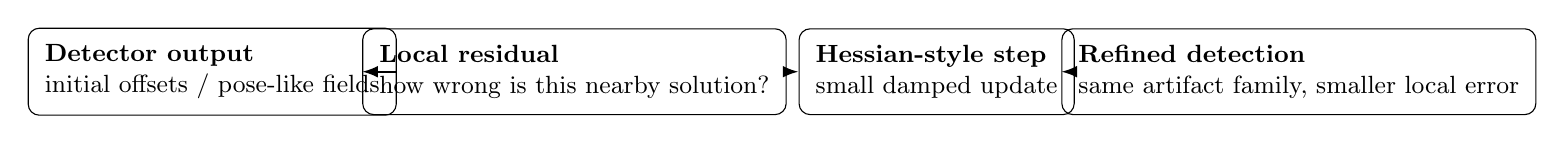
\begin{tikzpicture}[
  font=\small,
  box/.style={draw, rounded corners, align=left, inner sep=6pt},
  arrow/.style={-{Latex[length=2mm]}, thick}
]

\node[box] (pred) at (0,0) {\textbf{Detector output}\\initial offsets / pose-like fields};
\node[box] (res) at (4.6,0) {\textbf{Local residual}\\how wrong is this nearby solution?};
\node[box] (step) at (9.2,0) {\textbf{Hessian-style step}\\small damped update};
\node[box] (out) at (13.8,0) {\textbf{Refined detection}\\same artifact family, smaller local error};

\draw[arrow] (pred) -- (res);
\draw[arrow] (res) -- (step);
\draw[arrow] (step) -- (out);

\end{tikzpicture}
}
\caption{The practical picture: the model already produced an answer, and the Hessian solver asks whether a small local correction can make that answer geometrically cleaner.}
\end{figure}

\section{Plain-language intuition}
If gradient descent feels like following the local slope, Hessian-style refinement feels like also paying attention to the shape of the bowl around the current solution.

That is useful when the model is already close, but not quite aligned:
\begin{itemize}
  \item the center offset is slightly wrong,
  \item depth is plausible but biased,
  \item rotation is nearly correct but still misaligned.
\end{itemize}

In other words, this chapter is about \textbf{small local corrections}, not about teaching the model a whole new concept.

\section{Why pose workflows care}
Pose outputs are often more sensitive than plain detection outputs.
A box can still count as correct even when it is a little loose.
By contrast, pose-style outputs can degrade quickly when:
\begin{itemize}
  \item the center offset is wrong,
  \item the depth is slightly biased,
  \item the rotation is off by a small but important angle.
\end{itemize}

That is why the solver exists with pose use cases in mind, even though the current public CLI rollout deliberately starts from the safest operational target: \textbf{offset refinement}.

The broader design still reflects pose-oriented quantities:
\begin{itemize}
  \item depth-like variables,
  \item rotation-like variables,
  \item offsets,
  \item intrinsics-related corrections.
\end{itemize}

So the honest operational summary is:
\begin{itemize}
  \item \textbf{today's standard path}: offsets-first CLI refinement,
  \item \textbf{why it matters}: pose and geometry workflows often benefit from structured local correction.
\end{itemize}

\section{Optimal use cases}
Recommended applications include:
\begin{itemize}
  \item Offline validation and analysis scenarios where Ground Truth (GT) supervision or strict geometric constraints are accessible.
  \item Targeted error reduction specifically focused on highly difficult or anomalous samples.
  \item Post-inference refinement studies conducted subsequent to global calibration efforts.
\end{itemize}

It is strongly advised to avoid this technique by default in strict, real-time production environments due to the inherent latency overhead it introduces.

\section{CLI quickstart}
To enable refinement (opt-in behavior):
\begin{lstlisting}[language=bash]
python3 tools/refine_predictions_hessian.py \
  --predictions reports/predictions.json \
  --dataset data/smoke \
  --output reports/predictions_refined.json \
  --enable \
  --refine-offsets \
  --wrap
\end{lstlisting}

To explicitly disable refinement (pass-through behavior):
\begin{lstlisting}[language=bash]
python3 tools/refine_predictions_hessian.py \
  --predictions reports/predictions.json \
  --output reports/predictions_refined.json \
  --disable \
  --wrap
\end{lstlisting}

To enable refinement with customized solver parameters:
\begin{lstlisting}[language=bash]
python3 tools/refine_predictions_hessian.py \
  --predictions reports/predictions.json \
  --dataset data/smoke \
  --output reports/predictions_refined.json \
  --enable \
  --refine-offsets \
  --steps 10 \
  --damping 1e-2
\end{lstlisting}

\subsection{Workflow (misuse-prevention view)}
\begin{enumerate}
  \item Input predictions: \path{reports/predictions.json}
  \item Gate selection: \cmd{--disable} $\rightarrow$ pass-through, \cmd{--enable} $\rightarrow$ iterative refine
  \item Output predictions: \path{reports/predictions_refined.json}
  \item Validate output contract: \cmd{yolozu validate predictions reports/predictions_refined.json --strict}
\end{enumerate}

\section{Core configuration parameters}
Commonly tuned parameters (which correspond to the documentation in \path{docs/hessian_solver.md}):
\begin{itemize}
  \item \textbf{Gate/Control}: \cmd{--enable}/\cmd{--disable}, \cmd{steps}, \cmd{damping}, \cmd{fd_eps}
  \item \textbf{Target toggles}: \cmd{refine_offsets} (prioritizing offsets-first rollout)
  \item \textbf{Residual weights}: \cmd{w_depth}, \cmd{w_mask}, \cmd{w_reg}
  \item \textbf{Configuration file}: \cmd{--config <yaml|json>} (Note: CLI arguments will override config file values)
\end{itemize}

\section{Integration within the broader workflow}
A highly practical operational sequence is:
\begin{enumerate}
  \item Train the core model.
  \item Optionally execute dataset-wide calibration (addressing global scale and intrinsics).
  \item Apply Hessian refinement exclusively in scenarios where per-detection correction is demonstrably required.
\end{enumerate}

\section{Pros and Cons}
\textbf{Pros}
\begin{itemize}
  \item engine-external: it does not require changing the main inference graph,
  \item useful for offline analysis and controlled studies,
  \item especially intuitive for geometry-heavy predictions such as pose and depth.
\end{itemize}

\textbf{Cons}
\begin{itemize}
  \item it adds latency and is not a default real-time production path,
  \item it needs a meaningful residual to optimize,
  \item it can become numerically fragile without damping and step caps.
\end{itemize}

This chapter highlights the most frequently utilized parameters; for an exhaustive detailing of the parameter surface, please consult the tool's \cmd{--help} output, which is rigorously maintained in sync with the codebase.


\noindent\textbf{TensorRT Note:} TensorRT conversion strictly targets the inference graph execution. Hessian refinement functions as a completely separate, engine-external post-processing operation.

\chapter{Research Workflows (End-to-end Loops)}

\ChapterMeta{
This chapter defines repeatable research loops and the utilities for subsets, sweeps, and benchmarks.
}{
It keeps experiments artifact-first so results can be compared and regressed over time.
}{
It assumes stable JSON artifacts and, when needed, protocol presets. Keep subsets deterministic so comparisons stay fair and valid.
}
\ChapterAudience{Read this chapter when you are planning ablations, sweeps, offline distillation, or artifact-first research loops.}

\WorkflowOpening
{Run repeatable research loops while keeping the evaluation boundary artifact-first and comparable.}
{Use this for ablations, frozen subsets, protocol-pinned comparisons, sweeps, prediction distillation, and research notes.}
{Stable JSON artifacts, a fixed dataset subset or protocol, and explicit output paths for reports and histories.}
{Start with validation and protocol-pinned eval; use the specific sweep, distillation, or benchmark helper only after artifacts are valid.}
{Suite reports, sweep histories, distilled predictions, benchmark summaries, and research-note inputs.}
{Check that subset seeds, protocol files, metric keys, and artifact paths are recorded before interpreting the result.}
{Changing subsets mid-study, mixing conceptual and executable commands, skipping validation, or comparing reports with different protocol settings.}

\section{The research loop in \yolozu{}}
A canonical research iteration proceeds as follows:
\begin{enumerate}
  \item Build or acquire a model (either via internal training or external sourcing).
  \item Export predictions that follow the stable JSON interface contract.
  \item Validate artifacts immediately and fail fast.
  \item Evaluate the artifacts under a pinned protocol (generating suite reports).
  \item Run backend parity checks and compare historical runs with JSONL/CSV/MD histories.
  \item (Optional) Apply post-hoc calibration and then re-evaluate.
  \item (Optional) Execute hyperparameter sweeps and benchmark latency metrics.
\end{enumerate}

The discipline is simple: \textbf{treat artifacts as first-class entities}. Every run must generate JSON files that support reproduction and comparison.

\section{Freezing a dataset subset for ablations}
Rapid ablation studies frequently require a deterministic subset of a larger dataset. \yolozu{} provides a dedicated utility for this purpose:
\begin{lstlisting}[language=bash]
python3 tools/make_subset_dataset.py   --dataset data/coco128   --split train2017   --n 50   --seed 0   --out reports/coco128_50
\end{lstlisting}

This command writes:
\begin{itemize}
  \item A dedicated subset dataset directory.
  \item A frozen image list for reproducible sampling.
  \item A subset metadata JSON file for clear provenance.
\end{itemize}

\section{Protocol-pinned evaluation (YOLO26 example)}
Protocols pin evaluation settings so metrics remain comparable over time. For YOLO26, the protocol is defined in \path{protocols/yolo26_eval.json}; the evaluation tool reads this file and embeds its parameters into the final suite reports.

To execute a suite evaluation across multiple prediction artifacts:
\begin{lstlisting}[language=bash]
python3 tools/eval_suite.py   --protocol yolo26   --dataset /path/to/yolo-dataset   --predictions-glob '/path/to/pred_*.json'   --output reports/eval_suite.json
\end{lstlisting}

The resulting report includes protocol metadata, such as split definitions and bounding box formats. This metadata is required for valid research comparisons.

\section{Validating interface contracts as a research quality gate}
Before investing time in metric interpretation, you must validate your artifacts:
\begin{lstlisting}[language=bash]
python3 tools/validate_dataset.py --dataset /path/to/yolo --strict
python3 tools/validate_predictions.py /path/to/predictions.json --strict
\end{lstlisting}

This step is particularly critical when ingesting predictions exported from external pipelines.

\section{Backend parity (Torch vs. ONNX Runtime vs. TensorRT)}
When evaluating different inference backends, output alignment comes first. Use the parity tooling to compare two \path{predictions.json} artifacts and identify systematic differences, such as preprocessing, coordinate formatting, or numerical drift.

\textbf{Conceptual (not copy-paste as-is):} parity command shape.
Use real artifacts and validate them first as shown in the quality-gate section above.
\begin{lstlisting}[language=bash]
yolozu parity   --reference reports/pred_torch.json   --candidate reports/pred_onnxrt.json
\end{lstlisting}

\section{Sweeps (Hyperparameter search harness)}
Research workflows often need parameter sweeps that run outside the primary training loop. The sweep harness runs external commands, aggregates metrics, and writes summary tables.

Quick start:
\begin{lstlisting}[language=bash]
python3 tools/hpo_sweep.py --config docs/hpo_sweep_example.json --resume
\end{lstlisting}

Default outputs include:
\begin{itemize}
  \item \path{reports/hpo_sweep.jsonl}
  \item \path{reports/hpo_sweep.csv}
  \item \path{reports/hpo_sweep.md}
\end{itemize}

Use the \cmd{--resume} flag to make sweeps incremental and resilient to interruptions.

Critical configuration fields (detailed in \path{docs/hpo_sweep.md}):
\begin{itemize}
  \item \textbf{Required}: \cmd{base_cmd}, alongside either \cmd{param_grid} or \cmd{param_list}.
  \item \textbf{Optional}: \cmd{run_dir}, \cmd{metrics.path}, \cmd{metrics.keys}.
  \item \textbf{Optional outputs}: \cmd{result_jsonl}, \cmd{result_csv}, \cmd{result_md}.
  \item \textbf{Optional runtime controls}: \cmd{env}, \cmd{shell}.
\end{itemize}

The harness is intentionally framework-agnostic; it makes no assumptions about the underlying training stack.

\section{Prediction distillation workflow}
\yolozu{} includes a beginner-friendly \emph{offline prediction distillation} helper at
\path{tools/distill_predictions.py}. This section is intentionally written in the same spirit as the TTT chapter:
start from the goal, then follow the concrete procedure, then inspect the resulting artifacts.

\subsection{What this workflow is}
Prediction distillation in this chapter means:
\begin{itemize}
  \item take a \textbf{student} \path{predictions.json},
  \item take a \textbf{teacher} \path{predictions.json},
  \item compare them image-by-image,
  \item blend matched detections, optionally inject selected teacher-only detections,
  \item write a new distilled \path{predictions.json} plus a compact report.
\end{itemize}

The important point is that this is an \textbf{artifact-level} workflow.
It does \emph{not} update model weights. It is a fast research helper for answering:
\begin{quote}
``If I trust this teacher more than the student on this subset, is there enough signal to justify a heavier training-time distillation setup?''
\end{quote}

\subsection{What this workflow is not}
This section's \emph{prediction distillation} is narrower than the self-distillation discussed in the continual-learning chapter and narrower than TTT:
\begin{itemize}
  \item it is \textbf{not} checkpoint-based self-distillation during training,
  \item it is \textbf{not} an anti-forgetting method by itself,
  \item it is \textbf{not} changing model parameters at inference time,
  \item it is \textbf{not} a substitute for the full evaluator when reporting final numbers.
\end{itemize}

So the separation is:
\begin{itemize}
  \item \textbf{Prediction distillation}: rewrite one prediction artifact using another prediction artifact.
  \item \textbf{Self-distillation}: train a checkpoint while regularizing it toward another checkpoint.
  \item \textbf{TTT / CTTA}: adapt model parameters in memory during inference-time operation.
\end{itemize}

\begin{figure}[tbp]
\centering
\resizebox{0.94\linewidth}{!}{%
\begin{tikzpicture}[
  font=\small,
  box/.style={draw, rounded corners, align=left, inner sep=6pt},
  artifactbox/.style={box, fill=blue!8, text width=3.8cm},
  matchbox/.style={box, fill=orange!10, text width=4.4cm},
  actionbox/.style={box, fill=green!10, text width=3.8cm},
  outputbox/.style={box, fill=purple!8, text width=4.0cm},
  arrow/.style={-{Latex[length=2mm]}, thick}
]

\node[artifactbox] (student) at (0,2.45) {\textbf{Student artifact}\\\path{predictions_student.json}};
\node[artifactbox] (teacher) at (9.2,2.45) {\textbf{Teacher artifact}\\\path{predictions_teacher.json}};
\node[matchbox] (match) at (4.6,0.15) {\textbf{Match detections}\\same image, same class, IoU threshold};
\node[actionbox] (blend) at (0,-2.75) {\textbf{Blend matched scores}\\controlled by \cmd{--alpha}};
\node[actionbox] (inject) at (9.2,-2.75) {\textbf{Optionally inject teacher-only detections}\\guarded by score / duplicate / count caps};
\node[outputbox] (output) at (4.6,-5.55) {\textbf{Distilled artifacts}\\\path{predictions_distilled.json}\\\path{distill_report.json}};

\draw[arrow] (student) -- (match);
\draw[arrow] (teacher) -- (match);
\draw[arrow] (match) -- (blend);
\draw[arrow] (match) -- (inject);
\draw[arrow] (blend) -- (output);
\draw[arrow] (inject) -- (output);

\end{tikzpicture}
}
\caption{Prediction distillation flow in \yolozu{}: keep the student artifact as the base, borrow teacher signal under explicit rules, then emit a new distilled artifact instead of mutating the originals.}
\end{figure}

\subsection{A friendlier mental model}
If you need to explain this workflow to a new teammate, the most useful sentence is:
\begin{quote}
The student artifact is the first draft; the teacher artifact is the reviewer; distillation applies only a limited set of corrections and writes a new artifact.
\end{quote}

In practice, each candidate object lands in one of three buckets:
\begin{itemize}
  \item \textbf{Matched}: both student and teacher found the same object. This usually leads to a safer score update.
  \item \textbf{Teacher-only}: the teacher found an object that the student missed. This can improve recall, but it is also where false positives enter.
  \item \textbf{Student-only}: the student found an object that the teacher did not. The helper keeps the student artifact as the base.
\end{itemize}

\begin{figure}[h]
\centering
\resizebox{\linewidth}{!}{%
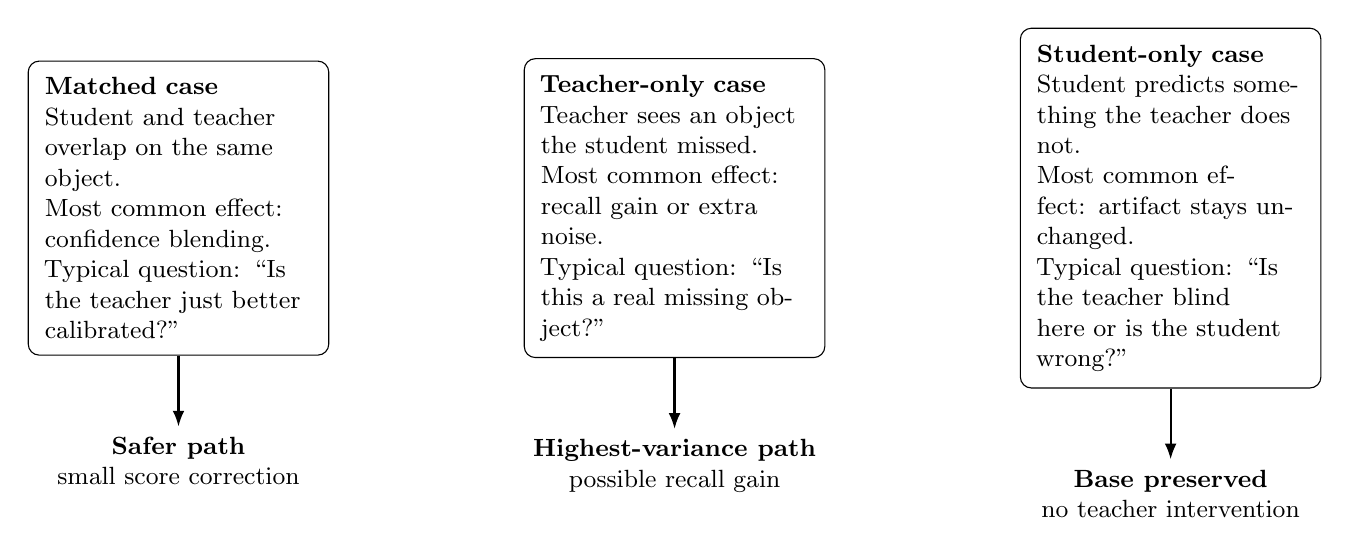
\begin{tikzpicture}[
  font=\small,
  box/.style={draw, rounded corners, align=left, inner sep=6pt, text width=0.28\linewidth},
  arrow/.style={-{Latex[length=2mm]}, thick}
]

\node[box] (matched) at (0,0) {\textbf{Matched case}\\Student and teacher overlap on the same object.\\Most common effect: confidence blending.\\Typical question: ``Is the teacher just better calibrated?''};
\node[box] (teacher) at (6.3,0) {\textbf{Teacher-only case}\\Teacher sees an object the student missed.\\Most common effect: recall gain or extra noise.\\Typical question: ``Is this a real missing object?''};
\node[box] (student) at (12.6,0) {\textbf{Student-only case}\\Student predicts something the teacher does not.\\Most common effect: artifact stays unchanged.\\Typical question: ``Is the teacher blind here or is the student wrong?''};

\draw[arrow] (matched.south) -- ++(0,-0.9) node[below, align=center] {\textbf{Safer path}\\small score correction};
\draw[arrow] (teacher.south) -- ++(0,-0.9) node[below, align=center] {\textbf{Highest-variance path}\\possible recall gain};
\draw[arrow] (student.south) -- ++(0,-0.9) node[below, align=center] {\textbf{Base preserved}\\no teacher intervention};

\end{tikzpicture}
}
\caption{The three cases to look for when reading a distillation result. For beginners, this is often easier to reason about than starting directly from the final metric table.}
\end{figure}

\subsection{Step-by-step procedure}
\paragraph{Step 1: Prepare two valid artifacts}
You need one student predictions artifact and one teacher predictions artifact.
Before distilling, validate both:
\begin{lstlisting}[language=bash]
python3 tools/validate_predictions.py reports/predictions_student.json --strict
python3 tools/validate_predictions.py reports/predictions_teacher.json --strict
\end{lstlisting}

For operator convenience, \cmd{tools/distill_predictions.py} also accepts wrapped payloads with partial \path{meta} blocks and supplements missing stable keys (for example \texttt{adapter}, \texttt{timestamp}, \texttt{tta}, \texttt{ttt}) before validation. This makes checked-in research artifacts easier to reuse without hand-editing metadata first.

\paragraph{Step 2: Decide how aggressive the blend should be}
The most important knobs are:
\begin{itemize}
  \item \cmd{--alpha}: how strongly matched detections move toward the teacher score.
  \item \cmd{--iou-threshold}: how much overlap teacher/student detections need before they count as the same object.
  \item \cmd{--add-missing}: whether teacher-only detections may be injected.
  \item \cmd{--teacher-min-score}: minimum confidence required before a teacher-only detection may be injected.
  \item \cmd{--max-added-per-image}: cap on teacher-only additions.
  \item \cmd{--add-duplicate-iou-threshold}: prevents near-duplicate teacher injections.
\end{itemize}

\paragraph{Safe-first reading strategy}
When in doubt, use this order:
\begin{enumerate}
  \item run a conservative pass first,
  \item inspect whether \path{matched} dominates \path{added},
  \item only then enable teacher-only injection,
  \item if \path{added} dominates but the visual result looks noisy, treat the gain as fragile.
\end{enumerate}

\paragraph{Step 3: Run a conservative first pass}
Start with a conservative run before enabling teacher-only injection:
\begin{lstlisting}[language=bash]
python3 tools/distill_predictions.py \
  --student reports/predictions_student.json \
  --teacher reports/predictions_teacher.json \
  --dataset data/coco128 \
  --split val2017 \
  --alpha 0.5 \
  --iou-threshold 0.7 \
  --output reports/predictions_distilled.json \
  --output-report reports/distill_report.json
\end{lstlisting}

\paragraph{Step 4: Run an exploratory ablation if needed}
If you want to test whether teacher-only detections help, enable guarded injection:
\begin{lstlisting}[language=bash]
python3 tools/distill_predictions.py \
  --student reports/predictions_student.json \
  --teacher reports/predictions_teacher.json \
  --dataset data/coco128 \
  --split val2017 \
  --alpha 0.5 \
  --iou-threshold 0.7 \
  --add-missing \
  --teacher-min-score 0.25 \
  --max-added-per-image 20 \
  --add-duplicate-iou-threshold 0.9 \
  --output reports/predictions_distilled.json \
  --output-report reports/distill_report.json
\end{lstlisting}

\paragraph{Step 4b: Prefer a checked-in YAML config when the CLI gets too long}
The helper also accepts \cmd{--config} in JSON or YAML format.
For day-to-day use, the shortest recommended boilerplate is the checked-in YAML file:
\path{configs/examples/distill_predictions.yaml}.

\begin{lstlisting}[language=bash]
python3 tools/distill_predictions.py \
  --student reports/predictions_student.json \
  --teacher reports/predictions_teacher.json \
  --dataset data/coco128 \
  --split val2017 \
  --config configs/examples/distill_predictions.yaml \
  --output reports/predictions_distilled.json \
  --output-report reports/distill_report.json
\end{lstlisting}

This is the preferred operator path when the long explicit flag list becomes hard to remember or copy correctly.

\paragraph{Step 5: Read the outputs in the right order}
The recommended reading order is:
\begin{enumerate}
  \item \path{distill_report.json}
  \item \path{predictions_distilled.json}
  \item a full evaluator report if the result looks promising
\end{enumerate}

\subsection{How the algorithm behaves}
\paragraph{Matched detections}
When teacher and student detections overlap enough under \cmd{--iou-threshold}, the helper treats them as corresponding detections and blends scores using \cmd{--alpha}.
This is usually the safer path because both artifacts already agree that there is probably an object there.

\paragraph{Teacher-only detections}
With \cmd{--add-missing}, the helper may inject detections that only the teacher predicted.
This is where gains and risks both tend to come from.

Typical upside:
\begin{itemize}
  \item recover missed objects,
  \item reveal useful teacher signal quickly.
\end{itemize}

Typical downside:
\begin{itemize}
  \item propagate teacher false positives,
  \item grow duplicate boxes when guardrails are too loose,
  \item overstate benefit on a tiny subset.
\end{itemize}

\subsection{How to read the report}
The compact report is enough for first-pass interpretation.
Inspect:
\begin{itemize}
  \item \path{losses.distill_score_gap}
  \item \path{metrics.student.map50}
  \item \path{metrics.student.map50_95}
  \item \path{metrics.distilled.map50}
  \item \path{metrics.distilled.map50_95}
  \item \path{meta.matched}
  \item \path{meta.added}
  \item \path{meta.distill.*}
\end{itemize}

Interpretation hints:
\begin{itemize}
  \item \textbf{high matched, low added}: mostly confidence refinement on objects both models found.
  \item \textbf{high added}: the result depends heavily on teacher-only injection.
  \item \textbf{metrics up with low added}: usually a healthier sign.
  \item \textbf{metrics up with very high added}: inspect duplicates and false positives carefully.
\end{itemize}

\subsection{Pros and Cons}
\begin{longtable}{@{}p{0.22\textwidth}p{0.33\textwidth}p{0.33\textwidth}@{}}
\toprule
\textbf{Workflow} & \textbf{Pros} & \textbf{Cons} \\
\midrule
Prediction distillation & Fast CPU-friendly ablation; no retraining required; preserves the predictions interface contract workflow; easy side-by-side artifact comparison & Post-hoc artifact rewrite only; gains can be fragile when injection dominates; does not solve forgetting by itself \\
\bottomrule
\end{longtable}

\subsection{Practical guardrails}
Recommended defaults for safer use:
\begin{itemize}
  \item keep \cmd{--teacher-min-score >= 0.2},
  \item keep \cmd{--max-added-per-image} finite,
  \item keep \cmd{--add-duplicate-iou-threshold} high (for example, \texttt{0.85}--\texttt{0.95}),
  \item specify \cmd{--split} when the dataset root has multiple candidate splits,
  \item treat the lightweight \cmd{simple_map} result as a \emph{quick signal}, not the final claim.
\end{itemize}

\subsection{When to use prediction distillation vs TTT vs self-distillation}
\begin{longtable}{@{}p{0.30\textwidth}p{0.56\textwidth}@{}}
\toprule
\textbf{Goal} & \textbf{Recommended workflow} \\
\midrule
Quick offline teacher/student ablation & Prediction distillation \\
Adapt at inference time under domain shift & TTT / CTTA \\
Mitigate forgetting while training across tasks/domains & Continual learning with self-distillation / replay / PEFT \\
Learn a new checkpoint that actually absorbs teacher behavior & Training-time distillation \\
\bottomrule
\end{longtable}

\subsection{Background references}
This helper is an artifact-level utility, not a claim of faithful reproduction of any single paper.
The conceptual lineage still comes from the broader distillation literature:
\begin{itemize}
  \item knowledge distillation: \cite{hinton2015distilling},
  \item self-distillation / Born-Again Networks: \cite{furlanello2018bornagain}.
\end{itemize}

Within research loops, prediction distillation is most useful as a \textbf{fast feasibility check}:
keep the dataset subset fixed, keep the downstream evaluator fixed, and use the distilled artifact to answer whether there is teacher signal worth pursuing further.

\section{Latency/FPS benchmarks with historical tracking (JSONL)}
Benchmark reports must be treated as formal artifacts. The latency harness generates a stable JSON report and can append results to a JSONL history file:
\begin{lstlisting}[language=bash]
python3 tools/benchmark_latency.py   --iterations 200   --warmup 20   --output reports/benchmark_latency.json   --history reports/benchmark_latency.jsonl   --notes 'baseline on target HW'
\end{lstlisting}

This dual-output pattern (a single JSON report coupled with a JSONL history) is invaluable for systematically tracking performance regressions across successive commits and varying hardware configurations.

\section{Run contract artifacts (Training research)}
When utilizing the in-repository trainer, it is strongly recommended to employ the contracted run mode to ensure the generation of consistent artifacts. This methodology is comprehensively detailed in Chapter~7 (Training and the Run Contract).

Minimal example:
\begin{lstlisting}[language=bash]
yolozu train configs/examples/train_contract.yaml --run-id exp01
\end{lstlisting}

Contracted outputs are systematically organized under \path{runs/exp01/} and encompass checkpoints, metrics JSONL files, ONNX exports, and parity reports.

\section{Notes on long-tail calibration experiments}
Post-hoc calibration frequently serves as a primary research axis. Utilize \cmd{yolozu calibrate} to generate calibrated prediction artifacts, enabling rigorous side-by-side comparisons of different methodologies. This process is thoroughly summarized in Chapter~6 (Score Calibration and Long-tail Adjustments).

\chapter{Continual Learning (Anti-forgetting)}

\ChapterMeta{
This chapter covers continual fine-tuning across tasks and domains, and the evaluation of forgetting using recorded run artifacts.
}{
It helps mitigate catastrophic forgetting and makes per-task metrics comparable over a training sequence.
}{
It requires continual configs and run artifacts (for example \cmd{continual_run.json}); optional replay and LoRA settings change compute and forgetting behavior.
}
\ChapterAudience{Read this chapter when you are training across tasks or domains and need to reason about forgetting, replay, self-distillation, LoRA, or QLoRA.}


\section{What YOLOZU means by ``continual''}
Continual learning (CL) here means fine-tuning across a sequence of tasks/domains while mitigating catastrophic forgetting.
In this repository, the reference implementation targets the in-repo \path{rtdetr_pose} scaffold.

\section{Core approach (baseline)}
The default strategy combines:
\begin{itemize}
  \item \textbf{Memoryless self-distillation}: keep the new model close to the previous checkpoint while learning the new task.
  \item \textbf{Optional replay buffer}: add a small buffer of past samples (e.g., reservoir sampling) and train on \emph{(current task + replay)}.
  \item \textbf{Optional parameter-efficiency}: restrict trainable parameters (e.g., LoRA) to reduce forgetting pressure.
\end{itemize}

\begin{figure}[h]
\centering
\resizebox{\linewidth}{!}{%
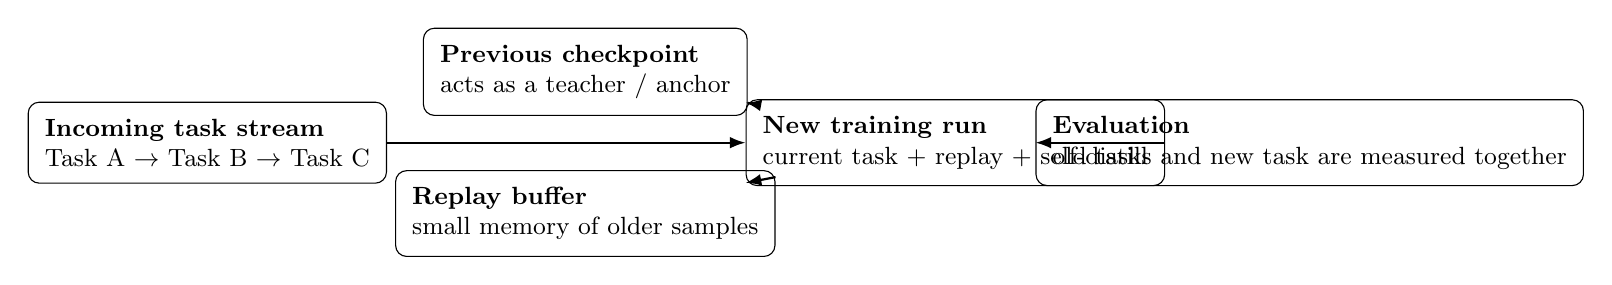
\begin{tikzpicture}[
  font=\small,
  box/.style={draw, rounded corners, align=left, inner sep=6pt},
  arrow/.style={-{Latex[length=2mm]}, thick}
]

\node[box] (tasks) at (0,0) {\textbf{Incoming task stream}\\Task A $\rightarrow$ Task B $\rightarrow$ Task C};
\node[box] (prev) at (4.8,0.9) {\textbf{Previous checkpoint}\\acts as a teacher / anchor};
\node[box] (replay) at (4.8,-0.9) {\textbf{Replay buffer}\\small memory of older samples};
\node[box] (train) at (9.5,0) {\textbf{New training run}\\current task + replay + self-distill};
\node[box] (eval) at (14.0,0) {\textbf{Evaluation}\\old tasks and new task are measured together};

\draw[arrow] (tasks) -- (train);
\draw[arrow] (prev) -- (train);
\draw[arrow] (replay) -- (train);
\draw[arrow] (train) -- (eval);

\end{tikzpicture}
}
\caption{Continual learning in \yolozu{}: the new run does not train on the latest task alone; it is anchored by the previous checkpoint and may also replay a small memory of older examples.}
\end{figure}

\section{LoRA / QLoRA in plain language}
LoRA and QLoRA are not separate continual-learning algorithms.
They are \textbf{ways to make the parameter updates smaller and cheaper}.

\subsection{LoRA}
The easiest mental model is:
\begin{quote}
freeze most of the big model, then train a much smaller correction on top.
\end{quote}

That is why LoRA is attractive in continual learning:
\begin{itemize}
  \item a smaller trainable surface can reduce forgetting pressure,
  \item it is often easier to fit within a limited GPU budget,
  \item it gives a more controlled ablation than full-model fine-tuning.
\end{itemize}

\subsection{QLoRA}
QLoRA keeps the same adapter idea, but stores the frozen base model in a more memory-efficient quantized form.

In plain language:
\begin{itemize}
  \item \textbf{LoRA}: freeze the large model, train small adapters.
  \item \textbf{QLoRA}: do the same thing, but keep the frozen base cheaper to hold in memory.
\end{itemize}

\begin{figure}[h]
\centering
\resizebox{\linewidth}{!}{%
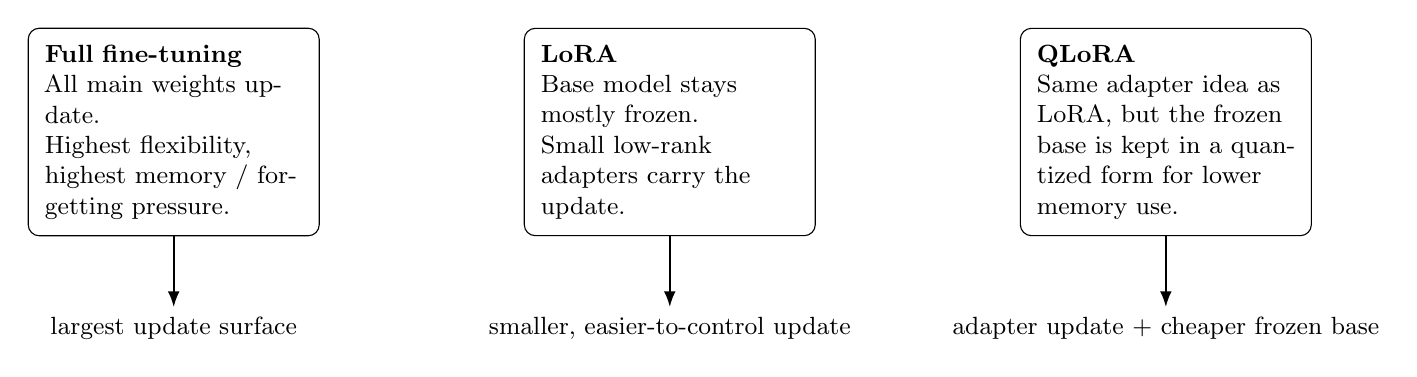
\begin{tikzpicture}[
  font=\small,
  box/.style={draw, rounded corners, align=left, inner sep=6pt, text width=0.27\linewidth},
  arrow/.style={-{Latex[length=2mm]}, thick}
]

\node[box] (base) at (0,0) {\textbf{Full fine-tuning}\\All main weights update.\\Highest flexibility, highest memory / forgetting pressure.};
\node[box] (lora) at (6.3,0) {\textbf{LoRA}\\Base model stays mostly frozen.\\Small low-rank adapters carry the update.};
\node[box] (qlora) at (12.6,0) {\textbf{QLoRA}\\Same adapter idea as LoRA, but the frozen base is kept in a quantized form for lower memory use.};

\draw[arrow] (base.south) -- ++(0,-0.9) node[below, align=center] {largest update surface};
\draw[arrow] (lora.south) -- ++(0,-0.9) node[below, align=center] {smaller, easier-to-control update};
\draw[arrow] (qlora.south) -- ++(0,-0.9) node[below, align=center] {adapter update + cheaper frozen base};

\end{tikzpicture}
}
\caption{LoRA and QLoRA are best understood as parameter-efficiency tools. They change \emph{how much} of the model moves during continual learning, not the underlying anti-forgetting objective itself.}
\end{figure}

\subsection{Pros and Cons}
\textbf{LoRA}
\begin{itemize}
  \item Pros: simpler mental model than QLoRA; often cheaper than full fine-tuning; integrates naturally with replay and self-distillation.
  \item Cons: still introduces extra knobs; can underfit if the adapter is too small; may hide the fact that the base model is the real bottleneck.
\end{itemize}

\textbf{QLoRA}
\begin{itemize}
  \item Pros: lowers memory pressure further; keeps the adapter-style workflow; attractive when the frozen base dominates footprint.
  \item Cons: adds quantization complexity; depends on backend support; is more experimental in this repository than plain LoRA.
\end{itemize}

\subsection{A practical choice example}
Imagine a domain-incremental warehouse-camera project:
\begin{itemize}
  \item the previous checkpoint is already usable,
  \item the main concern is forgetting older camera views,
  \item GPU memory is limited, but not critically constrained.
\end{itemize}

In that situation, \textbf{LoRA is usually the better first experiment}.
It keeps the story simpler: replay + self-distillation still do the anti-forgetting work, while the adapter merely reduces how much of the model moves.

Now change one assumption:
\begin{itemize}
  \item the frozen base is the real memory bottleneck,
  \item batch size collapses unless the base becomes cheaper to hold.
\end{itemize}

That is when \textbf{QLoRA becomes the practical option}.
You keep the same adapter-style update logic, but trade some simplicity for a smaller memory footprint.

So the operational rule is:
\begin{itemize}
  \item \textbf{LoRA first when clarity and debugging speed matter},
  \item \textbf{QLoRA when memory is the real blocker}.
\end{itemize}

\section{Main entry points}
\subsection{Train}
Run continual fine-tuning using a config (start from the example):
\begin{lstlisting}[language=bash]
python3 rtdetr_pose/tools/train_continual.py \
  --config configs/continual/rtdetr_pose_domain_inc_example.yaml
\end{lstlisting}

To run \textbf{memoryless} (no replay), set replay size to 0 in the config.

\paragraph{Note on "distillation" terminology}
This chapter's \emph{distillation} refers to \textbf{checkpoint-based self-distillation during training} (e.g., \cmd{--self-distill-from}) as an anti-forgetting mechanism.
The separate tool \path{tools/distill_predictions.py} performs \textbf{offline prediction blending} (rewriting a predictions JSON) and does not by itself mitigate catastrophic forgetting.

\subsection{Evaluate}
Evaluate forgetting and per-task metrics from the recorded run JSON:
\begin{lstlisting}[language=bash]
python3 tools/eval_continual.py \
  --run-json runs/continual/<run>/continual_run.json \
  --device cpu \
  --max-images 50
\end{lstlisting}

If your dataset provides pose sidecar metadata (e.g., under \path{labels/<split>/*.json}), you can request pose metrics:
\begin{lstlisting}[language=bash]
python3 tools/eval_continual.py \
  --run-json runs/continual/<run>/continual_run.json \
  --device cpu \
  --max-images 50 \
  --metric pose \
  --metric-key pose_success
\end{lstlisting}

Available \cmd{--metric-key} values in pose mode:
\begin{itemize}
  \item \cmd{pose_success}, \cmd{rot_success}, \cmd{trans_success}, \cmd{match_rate}, \cmd{iou_mean}
  \item \cmd{depth_abs_mean}, \cmd{depth_abs_median}
  \item \cmd{add_mean}, \cmd{add_median}, \cmd{adds_mean}, \cmd{adds_median}
\end{itemize}

Notes:
\begin{itemize}
  \item Depth metrics require GT depth/translation and predicted depth/translation fields.
  \item ADD/ADDS metrics require CAD points in sidecar metadata (\cmd{cad_points} / \cmd{cad_path} / \cmd{cad_points_path}) and valid GT+pred pose.
\end{itemize}

Examples for metric-key switching:
\begin{lstlisting}[language=bash]
# depth error summary
python3 tools/eval_continual.py \
  --run-json runs/continual/<run>/continual_run.json \
  --metric pose \
  --metric-key depth_abs_mean

# ADD / ADDS (requires CAD points)
python3 tools/eval_continual.py \
  --run-json runs/continual/<run>/continual_run.json \
  --metric pose \
  --metric-key add_mean

python3 tools/eval_continual.py \
  --run-json runs/continual/<run>/continual_run.json \
  --metric pose \
  --metric-key adds_mean
\end{lstlisting}

\section{Run artifacts (what to version / what to compare)}
\cmd{train_continual.py} writes a run folder under \path{runs/continual/}.
Key outputs:
\begin{itemize}
  \item \path{continual_run.json}: task list, checkpoints, config hash, and run record.
  \item \path{replay_buffer.json}: buffer summary (when replay is enabled).
  \item Per-task subfolders, typically including:\\
    \path{checkpoint.pt}, \path{metrics.jsonl}, \path{metrics.csv}, \path{run_record.json}.
\end{itemize}

For reporting and plots, treat \path{continual_run.json} as the single source of truth.

\section{Selected config knobs (high leverage)}
Commonly tuned items include:
\begin{itemize}
  \item Replay: \cmd{replay_size}, \cmd{replay_fraction}, \cmd{replay_per_task_cap}.
  \item Distillation: \cmd{distill.enabled}, \cmd{distill.keys}, \cmd{distill.weight}, \cmd{distill.temperature}.
  \item Replay distillation (DER++-style): \cmd{derpp.enabled} and related keys (requires teacher outputs stored in records).
  \item Regularizers across tasks (optional): EWC (\cmd{ewc.*}) and SI (\cmd{si.*}).
\end{itemize}

\section{Research workflow guidance}
\begin{itemize}
  \item \textbf{Pin the evaluation subset}: use a deterministic subset (same images each run) before comparing CL runs.
  \item \textbf{Log runtime cost}: replay and distillation change throughput; report accuracy vs cost.
  \item \textbf{Keep baselines simple}: compare (A) naive fine-tune, (B) memoryless self-distill, (C) replay+distill.
\end{itemize}

\section{Notes}
\begin{itemize}
  \item Some continual comparisons use a CPU-friendly proxy metric (e.g., a lightweight mAP-style summary) on a pinned subset to keep iteration fast.
  \item For ``real'' mAP, switch your evaluation workflow to a full COCO evaluator when appropriate.
\end{itemize}

\section{References (self-distillation background)}
This repository's checkpoint-based self-distillation is a pragmatic anti-forgetting regularizer.
For background reading:
\begin{itemize}
  \item Knowledge distillation (original): \cite{hinton2015distilling}.
  \item Self-distillation (classic reference): \cite{furlanello2018bornagain}.
  \item Continual learning via self-distillation (SDFT): \cite{shenfeld2026sdft}.
  \item LoRA as parameter-efficient tuning: \cite{hu2021lora}.
  \item QLoRA as quantized adapter tuning: \cite{dettmers2023qlora}.
\end{itemize}

\chapter{Test-Time Training (TTT): Tent, MIM, CoTTA, EATA, SAR}

\ChapterMeta{
This chapter explains controlled test-time adaptation (Tent/MIM/CoTTA/EATA/SAR), presets, guard rails, and reset policies for fair comparisons.
}{
It can improve robustness under domain shift by adapting weights in memory, while keeping cost bounded and results reproducible.
}{
It is most relevant when there is clear domain shift; comparisons require fixed image sets, bounded \cmd{--ttt-max-batches}, and careful seed and reset policy control.
}
\ChapterAudience{Read this chapter when you are adapting models under domain shift and want a method-by-method guide to Tent, MIM, CoTTA, EATA, and SAR.}

\paragraph{Readiness classification.}
TTT is a \textbf{research-oriented} lane in \yolozu{}.
Use it as an inference-time adaptation mode with bounded cost and explicit review, not as the default production update loop.
See \path{docs/production_readiness.md}.


\section{Scope and support}
\yolozu{} supports controlled test-time training (TTT) for the \path{rtdetr_pose} adapter via
\path{tools/export_predictions.py} or the unified wrapper \path{tools/yolozu.py}.

Authoritative references:
\begin{itemize}
  \item \path{docs/ttt_protocol.md}
  \item \path{docs/ttt_integration_plan.md}
  \item \path{docs/mim_inference.md}
\end{itemize}

TTT updates weights \emph{in memory} using unlabeled test data before (or during) inference \cite{sun2020ttt,wang2021tent}.
This makes comparisons sensitive to domain shift, random seeds, and reset policy.

\subsection{Plain-language glossary for this chapter}
Many readers first get stuck not on the code, but on the names. The short
meanings below are enough to read the rest of this chapter:
\begin{itemize}
  \item \textbf{TTA} (\textbf{Test-Time Augmentation}): run inference several times on simple transformed versions of the same image, then merge the predictions. This does \emph{not} update model weights.
  \item \textbf{TTT} (\textbf{Test-Time Training}): update some model parameters in memory at inference time using unlabeled test data.
  \item \textbf{CTTA} (\textbf{Continual Test-Time Adaptation}): a streaming form of TTT where adaptation continues over many incoming batches instead of resetting after every image.
  \item \textbf{LoRA}: a small trainable adapter added to selected layers, used when you want limited, safer parameter updates instead of moving the full model.
  \item \textbf{Norm-only update}: adapt only normalization-layer affine parameters (for example BatchNorm or LayerNorm scale/bias). This is one of the safest update scopes.
  \item \textbf{EMA} (\textbf{Exponential Moving Average}): a smoothed teacher copy of model weights. It changes more slowly than the student and is often used to stabilize adaptation.
  \item \textbf{Reset policy}: when and how the adapted weights are restored. \cmd{sample} means ``reset after each image/subset''; \cmd{stream} means ``carry updates forward across the stream.''
  \item \textbf{Guard rail}: a safety rule that limits adaptation, for example restricting which parameters may update or stopping updates when sample selection looks unreliable.
\end{itemize}

\paragraph{What the method names mean at a glance.}
\begin{itemize}
  \item \textbf{Tent}: minimize prediction entropy so the model becomes more confident on shifted inputs.
  \item \textbf{MIM}: use a masked-reconstruction objective so the model must infer hidden structure, not only sharpen confidence.
  \item \textbf{CoTTA}: a continual TTT method that combines student updates, an EMA-style teacher, augmentation agreement, and partial restoration so the model does not drift too far.
  \item \textbf{EATA}: an efficiency/reliability-oriented TTT method that adapts only on selected samples instead of updating on everything.
  \item \textbf{SAR}: a sharpness-aware robustness method; in practical terms, it tries to adapt in directions that are locally more stable instead of overreacting to noisy gradients.
\end{itemize}

\paragraph{How to read the rest of the chapter.}
If you only want the shortest reading path, use this order:
\begin{enumerate}
  \item understand whether you need \textbf{TTA} or \textbf{TTT},
  \item understand the \textbf{update scope} (norm-only, LoRA, or full-model),
  \item then compare the methods (Tent, MIM, CoTTA, EATA, SAR).
\end{enumerate}
This order matters because many failures blamed on the method are actually
caused by an overly broad update scope or an unsafe reset policy.

\subsection{Operator quick guide (read first)}
\begin{itemize}
  \item \textbf{Default OFF}: TTT is opt-in and only activates when \cmd{--ttt} is set.
  \item \textbf{Default update scope}: start with safe presets (norm-only / adapter-safe). For CoTTA/EATA/SAR rollout, keep updates constrained to LoRA/Norm-safe subsets first.
  \item \textbf{Reset recommendation}: for controlled comparisons, prefer \cmd{--ttt-reset sample}; for streaming latency operation, use bounded \cmd{--ttt-reset stream} with explicit \cmd{--ttt-max-batches}.
\end{itemize}

\begin{figure}[h]
\centering
\resizebox{0.95\linewidth}{!}{%
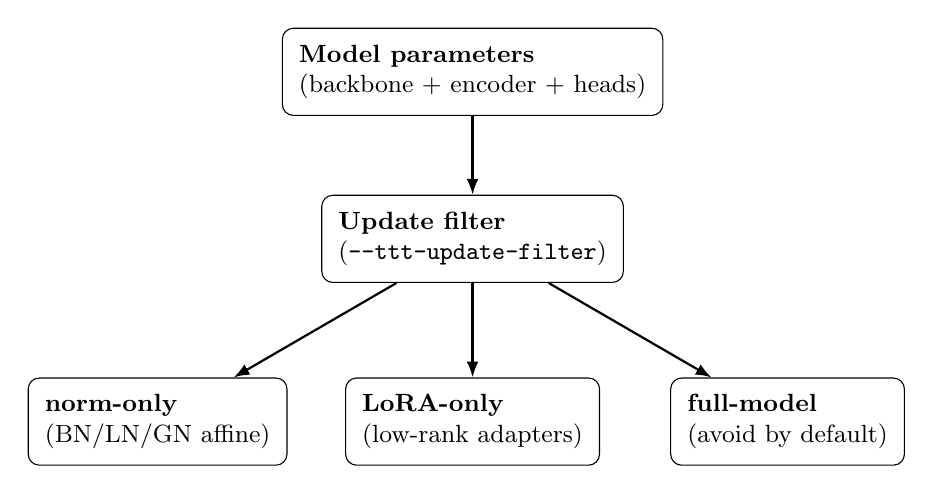
\begin{tikzpicture}[
  node distance=10mm,
  font=\small,
  box/.style={draw, rounded corners, align=left, inner sep=6pt},
  arrow/.style={-{Latex[length=2mm]}, thick}
]

\node[box] (all) {\textbf{Model parameters}\\(backbone + encoder + heads)};
\node[box, below=10mm of all] (filter) {\textbf{Update filter}\\(\cmd{--ttt-update-filter})};

\node[box, below=12mm of filter, xshift=-40mm] (norm) {\textbf{norm-only}\\(BN/LN/GN affine)};
\node[box, below=12mm of filter] (lora) {\textbf{LoRA-only}\\(low-rank adapters)};
\node[box, below=12mm of filter, xshift=40mm] (full) {\textbf{full-model}\\(avoid by default)};

\draw[arrow] (all) -- (filter);
\draw[arrow] (filter) -- (norm);
\draw[arrow] (filter) -- (lora);
\draw[arrow] (filter) -- (full);

\end{tikzpicture}
}
\caption{TTT update scope: start with constrained update filters (norm/LoRA) and keep full-model updates opt-in.}
\end{figure}

\section{When TTT is meaningful}
On clean COCO-style validation, TTT can be neutral or harmful.
To demonstrate improvements, you typically need a clear domain shift (e.g., corruptions, style shift, different camera).

Practical baseline:
\begin{itemize}
  \item Baseline domain: clean COCO \cmd{val2017}
  \item Target domain: shifted dataset or corrupted copy of COCO images
\end{itemize}

\subsection{Deterministic shift-target recipe}
For reproducible TTT evidence, generate a deterministic corrupted target split with:
\begin{lstlisting}[language=bash]
python3 scripts/prepare_ttt_domain_shift_target.py \
  --dataset-root data/smoke \
  --split val \
  --out reports/domain_shift/smoke_gaussian_blur_s2 \
  --corruption gaussian_blur \
  --severity 2 \
  --seed 2026 \
  --force
\end{lstlisting}

This produces \path{domain_shift_recipe.json} containing
\path{export_settings.domain_shift_target} with fixed
(\texttt{corruption}, \texttt{severity}, \texttt{seed}, \texttt{images\_sha256}).

To bind that recipe into prediction artifacts:
\begin{lstlisting}[language=bash]
python3 tools/export_predictions.py \
  --adapter dummy \
  --dataset reports/domain_shift/smoke_gaussian_blur_s2 \
  --split val \
  --wrap \
  --domain-shift-recipe reports/domain_shift/smoke_gaussian_blur_s2/domain_shift_recipe.json \
  --output reports/pred_shift_target.json
\end{lstlisting}

With \cmd{--wrap}, outputs explicitly include:
\begin{itemize}
  \item \path{meta.export_settings.domain_shift_target}
  \item \path{meta.export_settings.domain_shift_recipe} (\texttt{path}, \texttt{sha256})
\end{itemize}

\subsection{Real result summary: use this first}
The first thing beginners need is not a noisy overlay, but a controlled \emph{result summary}.
Figure~\ref{fig:ttt-real-summary} is therefore the primary onboarding figure for this chapter.
It uses the same few-shot checkpoint, the same ten shifted images, and the same seed for every method.
That means the bar chart is a controlled comparison, not a one-off anecdote.
The checked-in PNG figures are regenerated with \path{tools/render_ttt_manual_figures.py}.

Command summary (deterministic target + same checkpoint, with and without TTT):
\begin{lstlisting}[language=bash]
# 1) Prepare a deterministic shifted target split (1 image for illustration).
python3 scripts/prepare_ttt_domain_shift_target.py \
  --dataset-root data/smoke \
  --split val \
  --out reports/domain_shift/smoke_gaussian_blur_s3_1img \
  --corruption gaussian_blur \
  --severity 3 \
  --seed 2026 \
  --max-images 1 \
  --force

# 2) Inference overlays without TTT (torch backend + small repo-shipped checkpoint).
python3 tools/yolozu.py predict-images \
  --backend torch --device cpu \
  --config rtdetr_pose/configs/base.json \
  --checkpoint reports/rtdetr_pose_ckpt_coco128_gpu_matcher.pt \
  --image-size 320 --score-threshold 0.05 --max-detections 20 \
  --input-dir reports/domain_shift/smoke_gaussian_blur_s3_1img/images/val \
  --max-images 1 \
  --overlays-dir reports/ttt_demo/no_ttt_overlays \
  --output reports/ttt_demo/pred_no_ttt.json \
  --force

# 3) Same inference but with TTT enabled (Tent safe preset, reset per sample).
python3 tools/yolozu.py predict-images \
  --backend torch --device cpu \
  --config rtdetr_pose/configs/base.json \
  --checkpoint reports/rtdetr_pose_ckpt_coco128_gpu_matcher.pt \
  --image-size 320 --score-threshold 0.05 --max-detections 20 \
  --input-dir reports/domain_shift/smoke_gaussian_blur_s3_1img/images/val \
  --max-images 1 \
  --overlays-dir reports/ttt_demo/ttt_overlays \
  --output reports/ttt_demo/pred_ttt.json \
  --ttt --ttt-preset safe --ttt-reset sample --ttt-seed 2026 \
  --ttt-log-out reports/ttt_demo/ttt_log.json \
  --force
\end{lstlisting}

\begin{figure}[htbp]
  \centering
  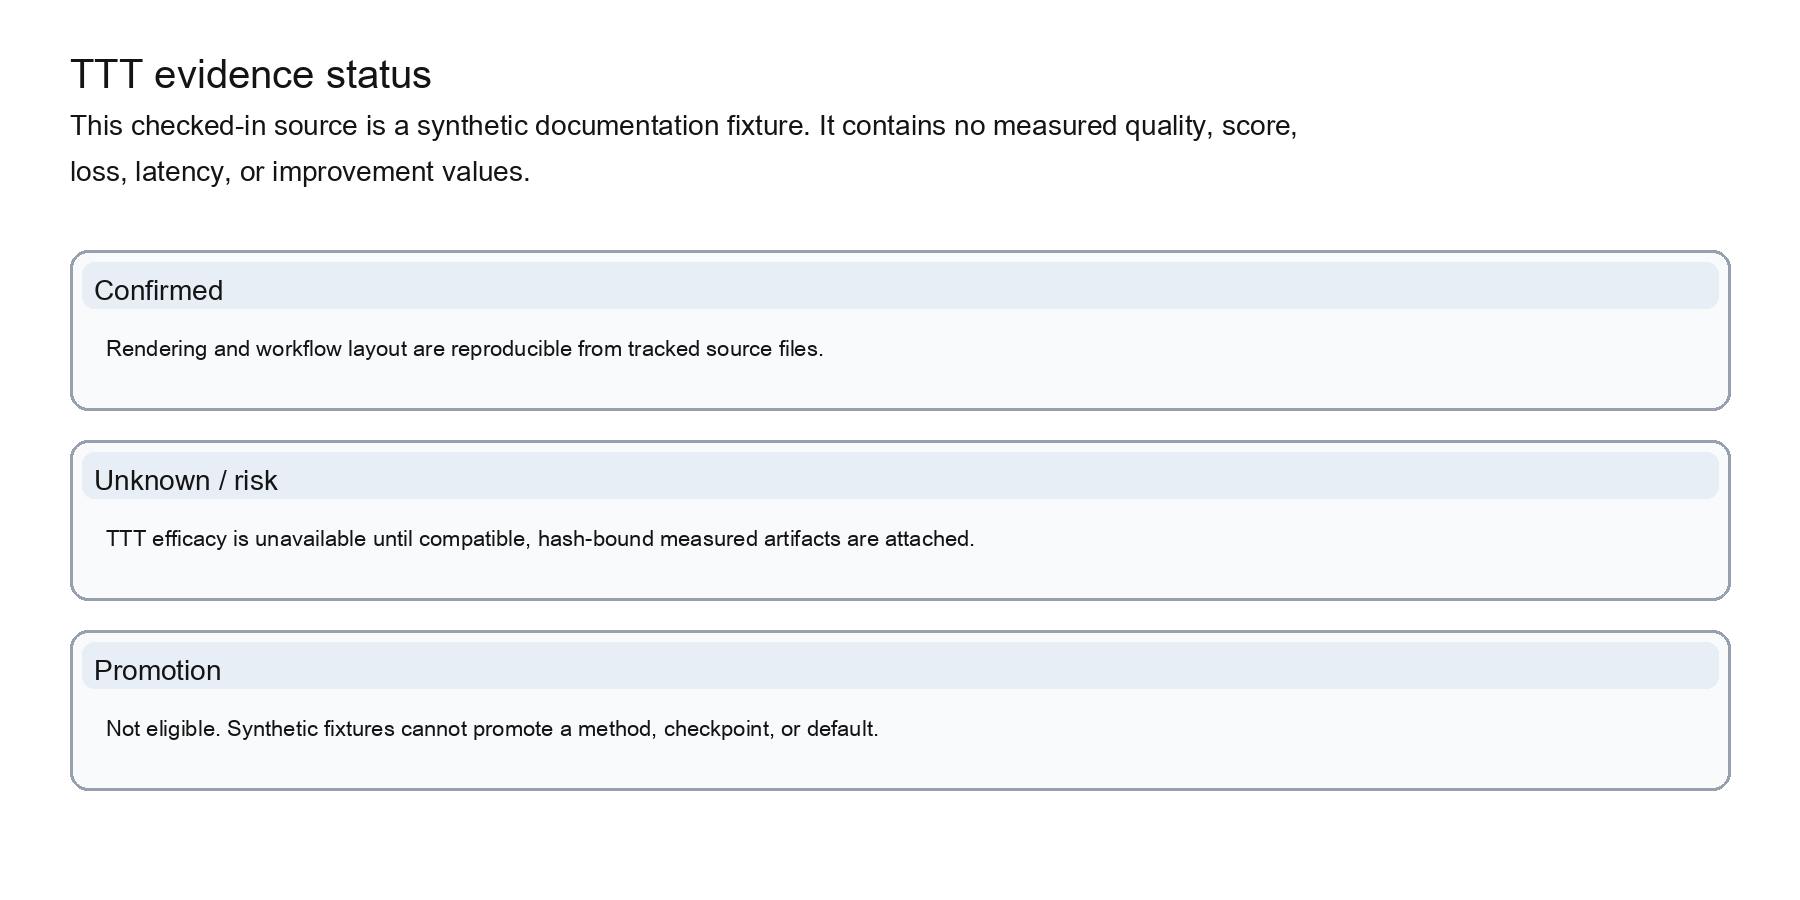
\includegraphics[width=\textwidth]{figures/ttt_method_results_summary.png}
  \caption{Primary TTT result figure. Real fixed-subset result summary from the ten-image shifted probe in \texttt{reports/ttt\_improvement\_probe}. Tent, CoTTA, EATA, and SAR all improve from \texttt{map50=0.00326797} to \texttt{0.00392157} and from \texttt{map50\_95=0.000326797} to \texttt{0.000392157} under the same checkpoint, subset, and seed. MIM is shown separately as execution evidence because the current repo-backed MIM smoke fixture proves the masked-reconstruction path runs (\texttt{steps\_run=2}, \texttt{mean\_final\_loss=0.461853}) but does not change exported detections on its tiny two-image smoke subset.}
  \label{fig:ttt-real-summary}
\end{figure}

\begin{figure}[htbp]
  \centering
  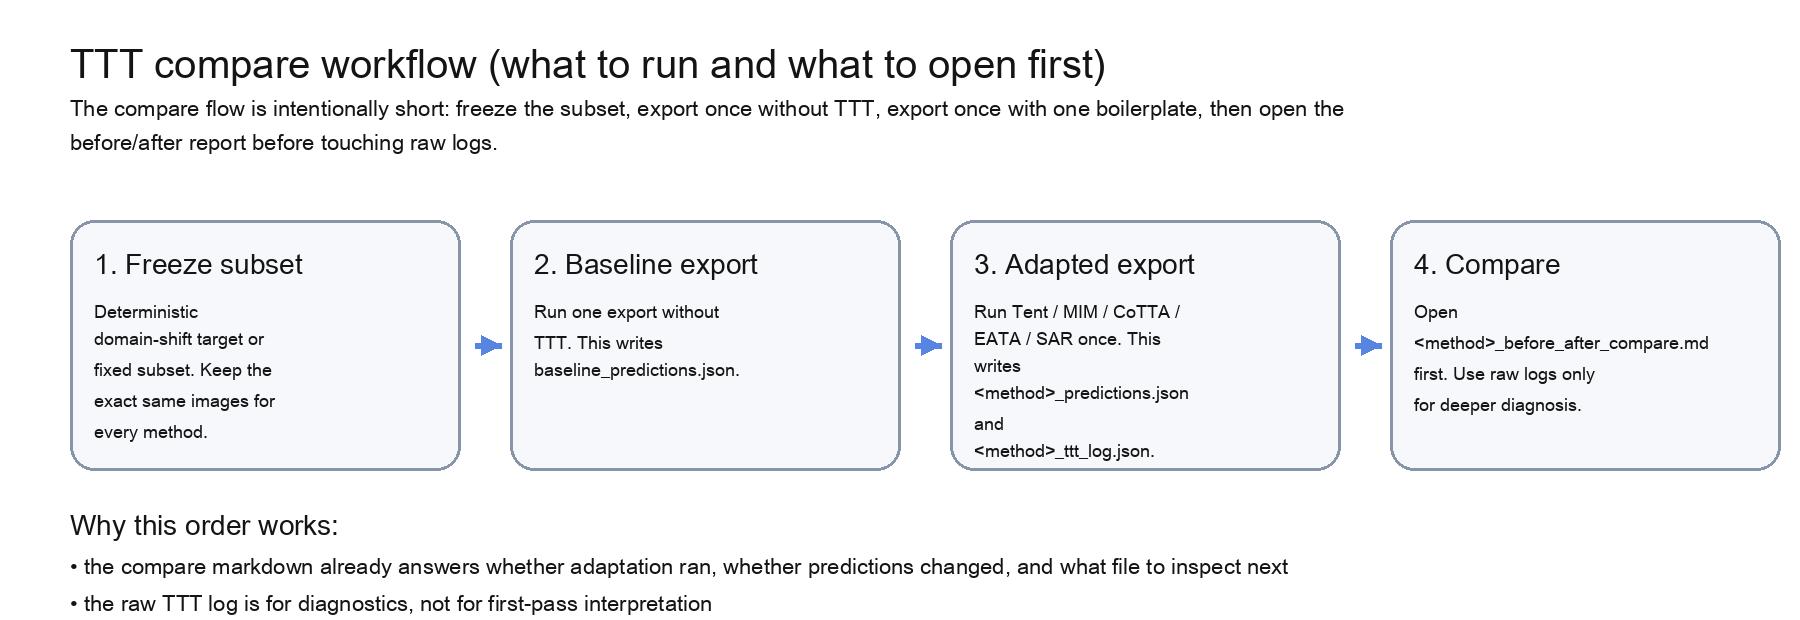
\includegraphics[width=\textwidth]{figures/ttt_compare_pipeline.png}
  \caption{Beginner-oriented processing flow for every TTT/CTTA method. Freeze the subset, export once without TTT, export once with one boilerplate, then open \texttt{<method>\_before\_after\_compare.md} before reading raw logs. This is the recommended reading order because the compare markdown answers whether adaptation actually ran, whether predictions changed, and which artifact to inspect next.}
  \label{fig:ttt-compare-workflow}
\end{figure}

\subsection{Metric micro-demo: show a delta (recommended)}
The visual example above shows \emph{what changes}. For onboarding and regression checks, it is also useful to show
\emph{a small metric delta} on a deterministic shift target.

\yolozu{} provides a self-contained micro-demo that:
\begin{itemize}
  \item trains a tiny few-shot checkpoint on clean \path{data/smoke} first (so no external weights download is required),
  \item applies a deterministic corruption to create a shifted target split,
  \item evaluates a simple mAP proxy for \textbf{no TTT} vs \textbf{with TTT} (and writes overlay PNGs).
\end{itemize}

\begin{lstlisting}[language=bash,caption={TTT improvement micro-demo: few-shot train + deterministic shift + metric delta.}]
# pip users:
python3 -m pip install -U 'yolozu[demo]'
yolozu demo ttt

# repo checkout equivalent:
python3 tools/yolozu.py demo ttt
\end{lstlisting}

Outputs include:
\begin{itemize}
  \item \path{demo_output/ttt/<utc>/ttt_improvement_report.json} (with \path{metrics.delta}),
  \item \path{demo_output/ttt/<utc>/overlay_no_ttt.png} and \path{overlay_ttt.png}.
\end{itemize}

Example stdout (CPU, deterministic seeds; values are intentionally tiny, the point is the reproducible delta):
\begin{itemize}
  \item \texttt{map50 0.00326797 $\to$ 0.00392157}
  \item \texttt{map50\_95 0.000326797 $\to$ 0.000392157}
\end{itemize}

\subsection{Per-image probe grid: concrete, but still secondary to the metric chart}
Figure~\ref{fig:ttt-qualitative-panel} uses the same fixed ten-image shifted subset as the metric summary.
It is intentionally secondary. The goal of this figure is not to prove quality with a single image, but to make the result concrete:
for each shifted image, it shows the top baseline detection, the top TTT detection, and the score movement.
This makes it much easier to explain what the detector is trying to localize and how the prediction changed, while the actual proof of improvement still comes from Figure~\ref{fig:ttt-real-summary}.

\begin{figure}[htbp]
  \centering
  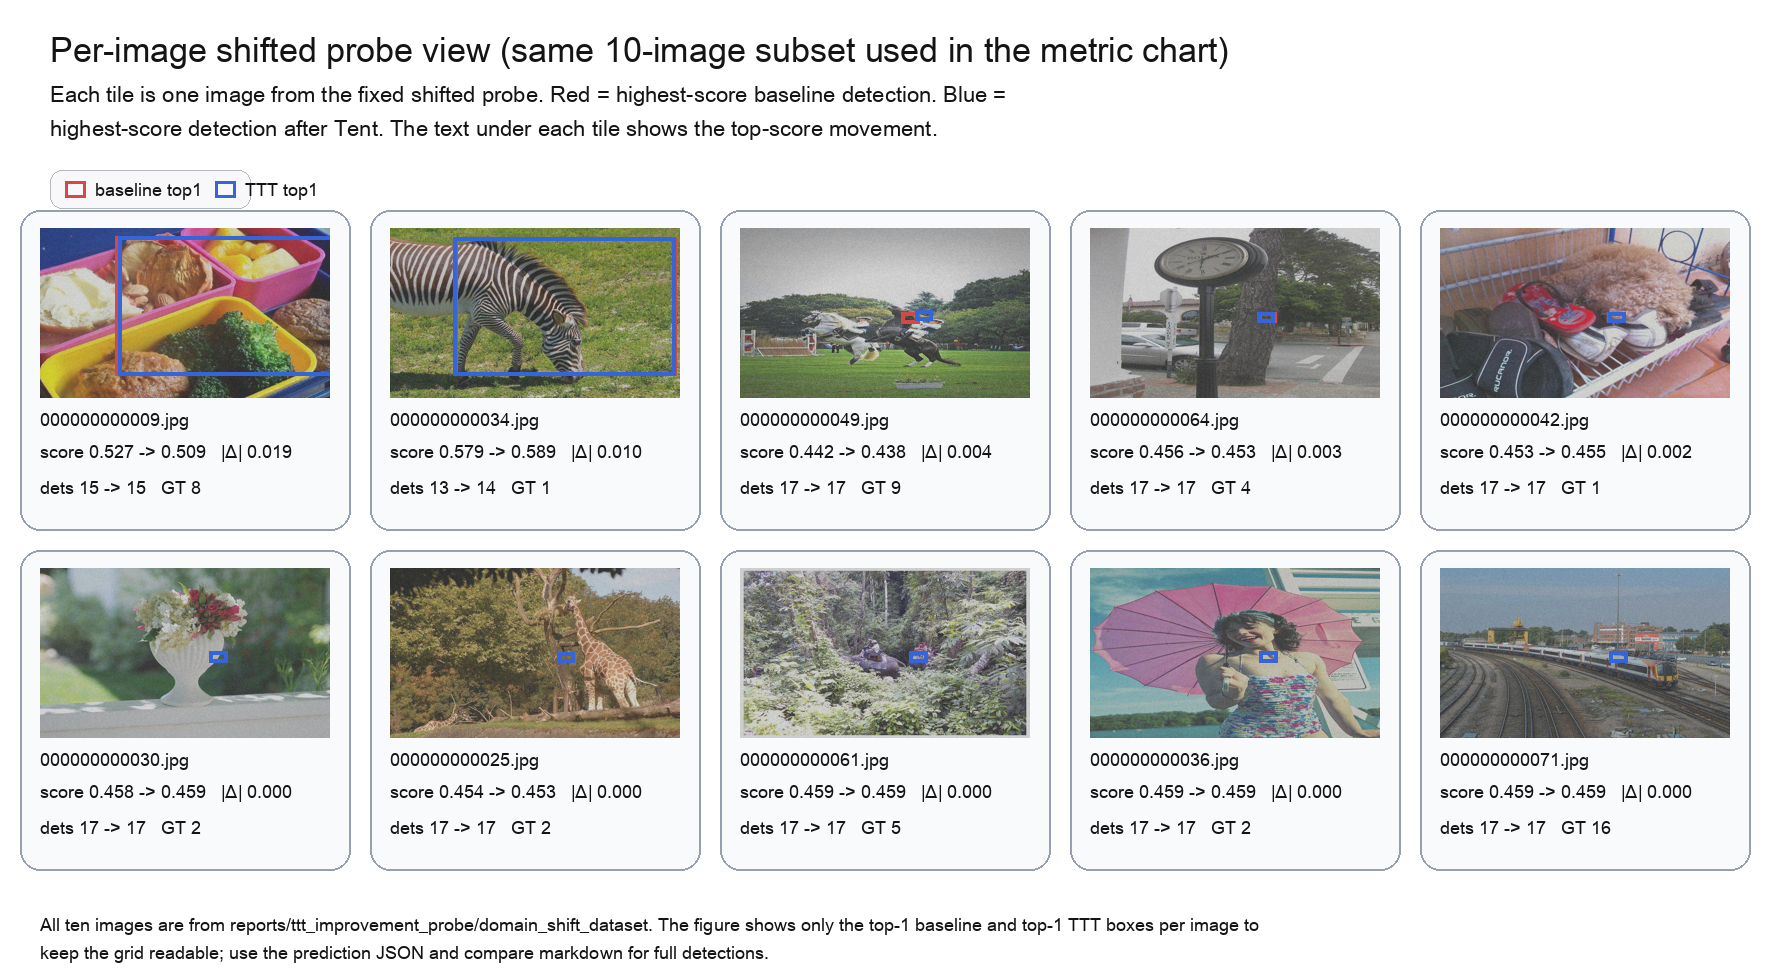
\includegraphics[width=\textwidth]{figures/ttt_probe_example_panel.png}
  \caption{Per-image result grid from the same fixed ten-image shifted probe used in Figure~\ref{fig:ttt-real-summary}. Each tile is one actual shifted image. Red marks the highest-score baseline detection without TTT; blue marks the highest-score detection after Tent. The text under each tile reports the top-score movement plus detection-count and ground-truth counts. This figure answers ``what was the detector trying to localize, and how did the top detection move on each image?'' The quantitative claim still comes from the fixed-subset metric chart in Figure~\ref{fig:ttt-real-summary}.}
  \label{fig:ttt-qualitative-panel}
\end{figure}

\section{Presets (start here)}
Both CLIs expose \cmd{--ttt-preset}:
\begin{itemize}
  \item \cmd{safe}: Tent + BN-affine only (\cmd{update_filter=norm_only})
  \item \cmd{adapter_only}: Tent + adapter/head only
  \item \cmd{mim_safe}: MIM + adapter/head only
  \item \cmd{cotta_safe}: CoTTA with conservative update/restore guard rails
  \item \cmd{eata_safe}: EATA selective adaptation with anti-forgetting defaults
  \item \cmd{sar_safe}: SAR LoRA-first sharpness-aware adaptation defaults
  \item \cmd{pose_safe}/\cmd{keypoints_safe}/\cmd{depth_safe}/\cmd{seg_safe}: task-aware Tent defaults
  \item \cmd{pose_mim}: pose-aware MIM defaults
\end{itemize}

Presets override core knobs (method, steps, lr, update filter, max batches) and set conservative guard rails unless you override them.
Use \cmd{--ttt-sdft-task \{pose,keypoints,depth,seg,full\}} and \cmd{--ttt-aux-*} weights to steer multi-task adaptation losses.

\section{Algorithm catalog with concrete examples}
The currently implemented parameter-updating TTT/CTTA methods are:
\cmd{tent}, \cmd{mim}, \cmd{cotta}, \cmd{eata}, and \cmd{sar}.
In practice, the fastest way to compare them fairly is:
\begin{enumerate}
  \item freeze the image subset,
  \item run the same adapter/checkpoint on the same shifted images,
  \item emit wrapped predictions for each method,
  \item compare method-specific logs and benchmark artifacts.
\end{enumerate}

\subsection{Recommended operator workflow: boilerplate compare}
Instead of retyping a long raw export command for each method, use the boilerplate compare wrapper:

\begin{lstlisting}[language=bash]
bash scripts/ttt_compare.sh \
  --boilerplate tent \
  --dataset data/smoke \
  --split val \
  --checkpoint /path/to.ckpt \
  --run-dir reports/ttt_compare/tent \
  --device cuda
\end{lstlisting}

This workflow writes:
\begin{itemize}
  \item \path{plan.json}
  \item \path{baseline_predictions.json}
  \item \path{<method>_predictions.json}
  \item \path{<method>_ttt_log.json}
  \item \path{<method>_before_after_compare.json}
  \item \path{<method>_before_after_compare.md}
\end{itemize}

The compare report provides the actual \textbf{before/after} summary:
baseline vs adapted prediction counts, TTT loss/runtime summary, and a compact drift summary
(\texttt{changed\_images}, \texttt{missing\_match\_failures}, \texttt{value\_mismatch\_failures}).

\subsection{Which files to compare for each method}
\begin{center}
\begin{tabular}{p{2.0cm} p{2.2cm} p{3.1cm} p{3.1cm} p{3.4cm}}
\toprule
\textbf{Method} & \textbf{Boilerplate} & \textbf{Baseline} & \textbf{Adapted} & \textbf{Primary before/after artifact} \\
\midrule
Tent & \cmd{tent} & \path{reports/ttt_compare/tent/baseline_predictions.json} & \path{reports/ttt_compare/tent/tent_predictions.json} & \path{reports/ttt_compare/tent/tent_before_after_compare.md} \\
MIM & \cmd{mim} & \path{reports/ttt_compare/mim/baseline_predictions.json} & \path{reports/ttt_compare/mim/mim_predictions.json} & \path{reports/ttt_compare/mim/mim_before_after_compare.md} \\
CoTTA & \cmd{cotta} & \path{reports/ttt_compare/cotta/baseline_predictions.json} & \path{reports/ttt_compare/cotta/cotta_predictions.json} & \path{reports/ttt_compare/cotta/cotta_before_after_compare.md} \\
EATA & \cmd{eata} & \path{reports/ttt_compare/eata/baseline_predictions.json} & \path{reports/ttt_compare/eata/eata_predictions.json} & \path{reports/ttt_compare/eata/eata_before_after_compare.md} \\
SAR & \cmd{sar} & \path{reports/ttt_compare/sar/baseline_predictions.json} & \path{reports/ttt_compare/sar/sar_predictions.json} & \path{reports/ttt_compare/sar/sar_before_after_compare.md} \\
\bottomrule
\end{tabular}
\end{center}

Recommended reading order:
\begin{enumerate}
  \item \path{plan.json} to confirm the frozen subset and boilerplate,
  \item \path{<method>\_before\_after\_compare.md} for the compact summary,
  \item \path{<method>\_ttt\_log.json} for adaptation loss/runtime details,
  \item method-specific follow-up tools only when deeper diagnostics are needed.
\end{enumerate}

\textbf{Important note.}
The shipped \cmd{mim} and \cmd{sar} boilerplates expand the safe defaults
directly and force
\cmd{--ttt-update-filter norm_only} so they run against the repo-shipped
checkpoint without requiring LoRA-specific weights. If a team owns a dedicated
adapter/LoRA checkpoint, it is better to copy the JSON boilerplate and switch
the update filter there than to fall back to a long raw CLI invocation.
The \cmd{mim} boilerplate also injects the repo-backed config
\path{configs/examples/ttt_compare/rtdetr_pose_mim_compare.json} into both the
baseline and adapted export commands so the MIM branch is enabled without a
manual config override.

\subsection{Smoke compare snapshot (repo-shipped checkpoint)}
We also validated the boilerplates against the repo-shipped checkpoint
\path{reports/rtdetr_pose_ckpt_coco128_gpu_matcher.pt} on \path{data/smoke},
\cmd{split=val}, \cmd{max-images=2}, \cmd{device=cpu}, with \cmd{--skip-eval}.

This is a workflow validation snapshot, not a quality claim. The tiny smoke
subset produced zero detections in both baseline and adapted runs, so the
useful signal here is method completion and the TTT log behavior.

\begin{table}[htbp]
\centering
\begin{tabular}{p{1.8cm} p{3.8cm} p{2.6cm} p{1.3cm} p{1.8cm}}
\toprule
\textbf{Method} & \textbf{Run dir} & \textbf{Real compare status} & \textbf{Steps} & \textbf{Mean final loss} \\
\midrule
Tent & \path{reports/ttt_compare/tent_smoke_cpu} & completed & 2 & 4.214431 \\
MIM & \path{reports/ttt_compare/mim_smoke_cpu} & completed & 2 & 0.461853 \\
CoTTA & \path{reports/ttt_compare/cotta_smoke_cpu} & completed & 1 & 4.243579 \\
EATA & \path{reports/ttt_compare/eata_smoke_cpu} & completed & 0 & null \\
SAR & \path{reports/ttt_compare/sar_smoke_cpu} & completed & 2 & 4.211009 \\
\bottomrule
\end{tabular}
\caption{Smoke compare snapshot for the repo-shipped checkpoint on \texttt{data/smoke}, \cmd{split=val}, \cmd{max-images=2}, \cmd{device=cpu}, with \cmd{--skip-eval}. This is a workflow-validation table, not a quality leaderboard. Warning notes are intentionally moved out of the table for readability: MIM uses the repo-backed compare config \texttt{configs/examples/ttt\_compare/rtdetr\_pose\_mim\_compare.json}; EATA reports \cmd{eata\_empty\_selected\_set} on both smoke images; Tent, CoTTA, and SAR complete without warnings on this smoke subset.}
\end{table}

For the completed runs, the compact summaries are:
\begin{itemize}
  \item \path{reports/ttt_compare/tent_smoke_cpu/tent_before_after_compare.md}
  \item \path{reports/ttt_compare/mim_smoke_cpu/mim_before_after_compare.md}
  \item \path{reports/ttt_compare/cotta_smoke_cpu/cotta_before_after_compare.md}
  \item \path{reports/ttt_compare/eata_smoke_cpu/eata_before_after_compare.md}
  \item \path{reports/ttt_compare/sar_smoke_cpu/sar_before_after_compare.md}
\end{itemize}

\subsection{How to read the smoke compare table}
The smoke table above is a \textbf{workflow validation table}. It tells you whether the method ran safely and emitted reproducible artifacts. It does \emph{not} claim that one method is globally better than another.

Read the columns in this order:
\begin{enumerate}
  \item \textbf{Real compare status}: did the whole compare workflow finish?
  \item \textbf{Steps}: how many adaptation updates actually ran?
  \item \textbf{Mean final loss}: what was the final adaptation objective value?
\end{enumerate}

Two common beginner mistakes:
\begin{itemize}
  \item treating \cmd{mean\_final\_loss} as a quality score across methods,
  \item treating \cmd{steps=0} as a failure.
\end{itemize}
Warning notes are now kept in the table caption rather than in a dedicated wide column.
For example, EATA can legitimately report \cmd{steps=0} with
\cmd{eata\_empty\_selected\_set}. That means the method decided \emph{not} to adapt on those smoke images, which is conservative behavior, not a crash.

\begin{figure}[h]
\centering
\resizebox{0.97\linewidth}{!}{%
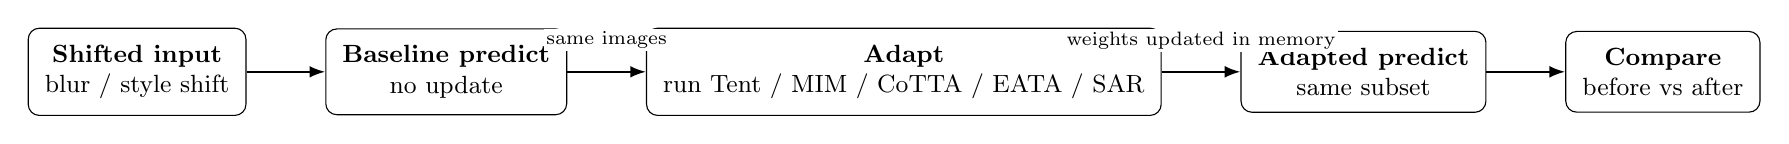
\begin{tikzpicture}[
  node distance=8mm,
  font=\small,
  box/.style={draw, rounded corners, align=center, inner sep=6pt, minimum width=24mm, fill=white},
  note/.style={align=center, font=\scriptsize, fill=white, inner sep=1pt},
  arrow/.style={-{Latex[length=2mm]}, thick}
]
\node[box] (input) {\textbf{Shifted input}\\blur / style shift};
\node[box, right=10mm of input] (base) {\textbf{Baseline predict}\\no update};
\node[box, right=10mm of base] (adapt) {\textbf{Adapt}\\run Tent / MIM / CoTTA / EATA / SAR};
\node[box, right=10mm of adapt] (pred) {\textbf{Adapted predict}\\same subset};
\node[box, right=10mm of pred] (cmp) {\textbf{Compare}\\before vs after};
\node[note] (sameimg) at ($(base.east)!0.5!(adapt.west)+(0,4mm)$) {same images};
\node[note] (weights) at ($(adapt.east)!0.5!(pred.west)+(0,4mm)$) {weights updated in memory};
\begin{pgfonlayer}{bg}
\draw[arrow] (input) -- (base);
\draw[arrow] (base) -- (adapt);
\draw[arrow] (adapt) -- (pred);
\draw[arrow] (pred) -- (cmp);
\end{pgfonlayer}
\end{tikzpicture}
}
\caption{Common TTT workflow in \yolozu{}: run the baseline and the adapted variant on the same deterministic image subset, then compare their artifacts.}
\end{figure}

\subsection{Operator workflow: what to do first}
For every method, the safest operator workflow is:
\begin{enumerate}
  \item choose a fixed dataset subset or a deterministic domain-shift target,
  \item run \path{scripts/ttt_compare.sh} with one boilerplate,
  \item open \path{<method>\_before\_after\_compare.md},
  \item only then inspect \path{<method>\_ttt\_log.json}.
\end{enumerate}

This order matters. The compare markdown is the onboarding artifact. It answers the first three questions operators usually have:
\begin{itemize}
  \item Did adaptation actually run?
  \item Did predictions change?
  \item Which file should I inspect next?
\end{itemize}

\subsection{Tent}
\textbf{What the name means.}
Tent is short for \textbf{fully Test-time adaptation by ENTropy minimization}.
The name is useful because it already tells you the two essential ideas:
\begin{itemize}
  \item adaptation happens at \emph{test time},
  \item entropy is the signal being minimized.
\end{itemize}

\textbf{Principle.}
Tent minimizes prediction entropy online using a restricted parameter subset \cite{wang2021tent}. In plain language, it pushes the model toward making sharper, more confident predictions on shifted inputs, but only lets a small subset of parameters move.

\textbf{What entropy means here.}
If a prediction spreads probability mass across many classes, the entropy is high.
If the same prediction becomes concentrated on one class, the entropy is low.
For a single prediction vector $p$, the usual entropy term is:
\[
H(p) = - \sum_c p_c \log p_c.
\]
Tent adapts a small subset of parameters by reducing the average prediction entropy over the selected test-time samples:
\[
\min_{\theta_{\mathrm{adapt}}} \; \mathrm{E}_{x \sim \mathrm{test\ stream}} \left[ H\!\left(p_{\theta}(y \mid x)\right) \right].
\]
In \yolozu{}'s safe presets, $\theta_{\mathrm{adapt}}$ is intentionally small, usually norm-affine parameters or a restricted adapter/head subset.

\textbf{Why it can work.}
Under mild domain shift, the model often still attends to roughly the right object, but its output distribution becomes softer and less decisive.
Tent exploits that situation: it does not ask the model to discover a brand-new concept, it only asks whether a more confident local decision boundary gives a better answer.

\textbf{What it is not.}
\begin{itemize}
  \item It is not supervised fine-tuning.
  \item It does not tell the model which class is correct.
  \item It assumes ``become more confident'' is a useful direction on the current shifted sample.
\end{itemize}

\begin{figure}[h]
\centering
\resizebox{0.95\linewidth}{!}{%
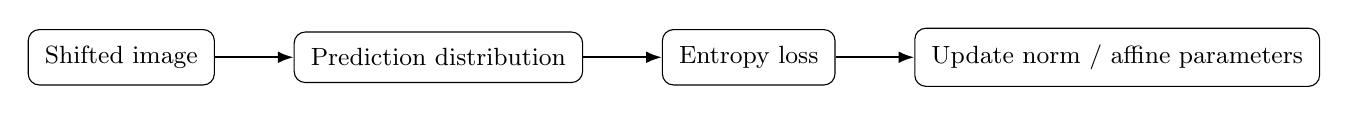
\begin{tikzpicture}[
  node distance=8mm,
  font=\small,
  box/.style={draw, rounded corners, align=center, inner sep=6pt},
  arrow/.style={-{Latex[length=2mm]}, thick}
]
\node[box] (x) {Shifted image};
\node[box, right=10mm of x] (p) {Prediction distribution};
\node[box, right=10mm of p] (h) {Entropy loss};
\node[box, right=10mm of h] (u) {Update norm / affine parameters};
\draw[arrow] (x) -- (p);
\draw[arrow] (p) -- (h);
\draw[arrow] (h) -- (u);
\end{tikzpicture}
}
\caption{Tent: use prediction entropy as the adaptation signal and keep updates constrained to a safe parameter subset.}
\end{figure}

\textbf{When to use it.}
Tent is the best first method. Choose it when you want the smallest operational jump away from baseline inference and the easiest debug path.

\textbf{Concrete procedure.}
\begin{lstlisting}[language=bash]
bash scripts/ttt_compare.sh \
  --boilerplate tent \
  --dataset data/smoke \
  --split val \
  --checkpoint /path/to.ckpt \
  --run-dir reports/ttt_compare/tent \
  --device cuda
\end{lstlisting}

\textbf{How to read the result.}
\begin{itemize}
  \item Open \path{tent\_before\_after\_compare.md} first.
  \item Check whether \cmd{steps\_run > 0}.
  \item If \cmd{changed\_images=0}, adaptation completed but exported predictions did not change on this subset.
  \item Open \path{tent\_ttt\_log.json} only if you need guard or runtime detail.
\end{itemize}

\textbf{Concrete repo result.}
On the fixed ten-image shifted probe in Figure~\ref{fig:ttt-real-summary}, Tent improves
\texttt{map50} from \texttt{0.00326797} to \texttt{0.00392157} and
\texttt{map50\_95} from \texttt{0.000326797} to \texttt{0.000392157}.
The effect is small, but it is reproducible under the same checkpoint, subset, and seed.

\textbf{Pros.}
\begin{itemize}
  \item easiest method to explain,
  \item cheapest adaptation cost,
  \item safest default when using norm-only updates.
\end{itemize}

\textbf{Cons.}
\begin{itemize}
  \item weakest self-supervised signal,
  \item can sharpen wrong predictions under severe shift,
  \item often less expressive than reconstruction-based methods.
\end{itemize}

\subsection{MIM}
\textbf{What the name means.}
MIM stands for \textbf{Masked Image Modeling}.
In plain language, we deliberately hide part of the visual signal and ask the model to reconstruct or predict what is missing.
That is why MIM feels more structural than Tent: it is not only asking for confidence, it is asking for internal consistency.

\textbf{Principle.}
MIM uses masked reconstruction and optional entropy terms to adapt from unlabeled shifted inputs. Instead of only asking the model to become more confident, it also asks the model to reconstruct hidden structure from partially masked internal features. The lineage is broader than MAE alone: denoising autoencoders already used corruption-plus-reconstruction as a representation-learning signal in 2008 \cite{vincent2008dae}, image inpainting-style reconstruction was used as a visual self-supervised task in Context Encoders \cite{pathak2016context}, and modern masked-image-modeling references include Masked Autoencoders (MAE) \cite{he2022mae} and SimMIM \cite{xie2022simmim}. For direct test-time usage, representative references are Test-Time Training with Masked Autoencoders \cite{gandelsman2022tttmae} and TTT-MIM \cite{mansour2024tttmim}. \yolozu{} uses this family of masked-image-modeling ideas as an inference-time auxiliary signal rather than as a standalone pretraining recipe.

\textbf{Minimal objective view.}
Let $M$ denote a mask and $R_{\theta}$ denote the reconstruction path.
A simplified masked-reconstruction loss can be written as:
\[
L_{\mathrm{MIM}} = \left\| R_{\theta}\!\left((1-M)\odot x\right) - M \odot x \right\|.
\]
Many practical test-time variants combine this reconstruction term with an entropy term:
\[
L_{\mathrm{adapt}} = \lambda_{\mathrm{mim}} L_{\mathrm{MIM}} + \lambda_{\mathrm{ent}} H\!\left(p_{\theta}(y \mid x)\right).
\]
The exact target differs across implementations, but the operational story stays the same:
\begin{itemize}
  \item hide part of the signal,
  \item ask the model to infer the hidden structure,
  \item use that self-supervised error as the adaptation signal.
\end{itemize}

\textbf{Research lineage and IP note.}
This manual cites representative prior-art waypoints so that operators can place the method in a broader technical lineage instead of treating MIM-style adaptation as a single new idea. The broad pattern---corrupt or mask part of the input/feature state, reconstruct hidden structure, and use that self-supervised loss to improve robustness---predates the current wording of test-time masked adaptation. This note is meant to support technical due diligence and prior-art positioning only; it is \textbf{not} legal advice and it is \textbf{not} a non-infringement opinion. Any deployment-specific IP or patent review belongs to qualified counsel.

\textbf{Why it can work.}
Entropy-only adaptation can be too weak when the shift is geometric, structural, or pose-sensitive.
MIM adds a denser self-supervised objective: the model is rewarded not merely for being decisive, but for reconstructing a plausible hidden structure from incomplete evidence.
That is why MIM is often easier to justify in pose-heavy workflows than plain confidence sharpening.

\textbf{What it is not.}
\begin{itemize}
  \item It is not just ``MAE pretraining at inference time''.
  \item It is not guaranteed to improve every exported detection.
  \item It is usually more model-specific than Tent because the masked-reconstruction branch must exist and stay numerically stable.
\end{itemize}

\begin{figure}[h]
\centering
\resizebox{0.97\linewidth}{!}{%
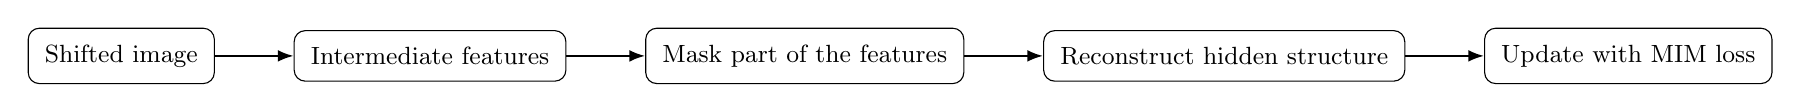
\begin{tikzpicture}[
  node distance=8mm,
  font=\small,
  box/.style={draw, rounded corners, align=center, inner sep=6pt},
  arrow/.style={-{Latex[length=2mm]}, thick}
]
\node[box] (x) {Shifted image};
\node[box, right=10mm of x] (f) {Intermediate features};
\node[box, right=10mm of f] (m) {Mask part of the features};
\node[box, right=10mm of m] (r) {Reconstruct hidden structure};
\node[box, right=10mm of r] (u) {Update with MIM loss};
\draw[arrow] (x) -- (f);
\draw[arrow] (f) -- (m);
\draw[arrow] (m) -- (r);
\draw[arrow] (r) -- (u);
\end{tikzpicture}
}
\caption{MIM: use masked reconstruction to create a stronger adaptation signal than entropy alone.}
\end{figure}

\textbf{When to use it.}
Choose MIM when you need a stronger adaptation signal than Tent, especially for pose-heavy or geometry-sensitive runs.

\textbf{Concrete procedure.}
\begin{lstlisting}[language=bash]
bash scripts/ttt_compare.sh \
  --boilerplate mim \
  --dataset data/smoke \
  --split val \
  --checkpoint /path/to.ckpt \
  --run-dir reports/ttt_compare/mim \
  --device cuda
\end{lstlisting}

For pose-heavy runs, switch to \cmd{--ttt-preset pose_mim}. \yolozu{} now ships
two practical MIM entrypoints:
\begin{itemize}
  \item \cmd{mim}: a repo-backed smoke fixture for verifying that the masked-reconstruction path is wired correctly
  \item \cmd{mim\_probe}: a fixed real probe that demonstrates an actual before/after metric delta on the bundled shifted ten-image probe
\end{itemize}

\begin{lstlisting}[language=bash]
bash scripts/ttt_compare.sh \
  --boilerplate mim \
  --dataset data/smoke \
  --split val \
  --checkpoint reports/rtdetr_pose_ckpt_coco128_gpu_matcher.pt \
  --run-dir reports/ttt_compare/mim_smoke_cpu \
  --device cpu \
  --max-images 2 \
  --skip-eval \
  --force
\end{lstlisting}

\textbf{Fixed real-probe compare.}
\begin{lstlisting}[language=bash]
bash scripts/ttt_compare.sh \
  --boilerplate mim_probe \
  --dataset reports/ttt_improvement_probe/domain_shift_dataset \
  --split val \
  --checkpoint reports/ttt_improvement_probe/checkpoint.pt \
  --run-dir reports/ttt_compare/mim_probe_cpu \
  --device cpu \
  --max-images 10
\end{lstlisting}

\textbf{How to read the result.}
\begin{itemize}
  \item Open \path{mim\_before\_after\_compare.md} first.
  \item Then inspect \path{mim\_ttt\_log.json}; the MIM loss trace is more informative than Tent's entropy-only loss.
  \item The repo-backed smoke example proves execution: \cmd{steps\_run=2}, \cmd{mean\_final\_loss=0.461853}, and \cmd{changed\_images=0 / 2}.
  \item The fixed real probe proves operator-visible impact: \cmd{steps\_run=10}, \cmd{mean\_final\_loss=0.0791513}, \cmd{changed\_images=10 / 10}, \cmd{map50 0.00326797 \rightarrow 0.00392157}, and \cmd{map50\_95 0.000326797 \rightarrow 0.000392157}.
  \item When \cmd{pycocotools} is not installed in the current runtime, the compare falls back to \cmd{simple\_map\_proxy} instead of silently skipping evaluation.
\end{itemize}

\textbf{Concrete repo results.}
\begin{itemize}
  \item repo-backed smoke compare: \cmd{steps\_run=2}, \cmd{mean\_final\_loss=0.461853}, \cmd{changed\_images=0 / 2}
  \item fixed real probe compare: \cmd{steps\_run=10}, \cmd{mean\_final\_loss=0.0791513}, \cmd{changed\_images=10 / 10}
  \item fixed real probe metrics: \cmd{map50 0.00326797 \rightarrow 0.00392157}, \cmd{map50\_95 0.000326797 \rightarrow 0.000392157}
\end{itemize}

\textbf{Pros.}
\begin{itemize}
  \item stronger self-supervised signal than Tent,
  \item useful for geometry- and pose-sensitive adaptation,
  \item easier to justify when confidence-only adaptation is too weak.
\end{itemize}

\textbf{Cons.}
\begin{itemize}
  \item more model-specific than Tent,
  \item more complex to interpret,
  \item loss values are not directly comparable to Tent values.
\end{itemize}

\subsection{CoTTA}
\textbf{What the name means.}
CoTTA is short for \textbf{Continual Test-Time Adaptation}.
The name matters because it signals that this method is designed for a stream, not just for a single isolated image.

\textbf{Principle.}
CoTTA combines augmentation-averaged predictions, EMA teacher updates, and stochastic restoration. The main idea is to adapt continuously in a stream while preventing the model from drifting too far.

\textbf{Minimal objective view.}
CoTTA can be read as a consistency objective between an online student and an EMA teacher across augmented views:
\[
L_{\mathrm{CoTTA}} = \sum_{a \in \mathcal{A}} d\!\left(p_{\theta}(y \mid a(x)),\; p_{\theta^{\mathrm{EMA}}}(y \mid x)\right).
\]
The exact distance term $d(\cdot,\cdot)$ and restoration schedule vary by implementation, but the operational story is stable:
\begin{itemize}
  \item smooth the target with an EMA teacher,
  \item average over augmented views,
  \item periodically restore part of the student so drift does not grow unchecked.
\end{itemize}

\textbf{Why it can work.}
Pure online adaptation can slowly walk away from a good solution in long streams.
CoTTA adds three safeguards against that:
\begin{itemize}
  \item augmentation averaging,
  \item EMA teacher smoothing,
  \item partial restoration of older weights.
\end{itemize}

\textbf{What it is not.}
\begin{itemize}
  \item It is not the simplest first TTT baseline.
  \item It is not stateless; stream order matters more than in per-sample adaptation.
  \item It makes the most sense when stream behavior itself is part of the problem.
\end{itemize}

\begin{figure}[h]
\centering
\resizebox{0.97\linewidth}{!}{%
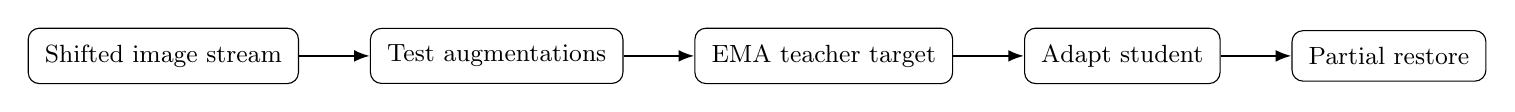
\begin{tikzpicture}[
  node distance=8mm,
  font=\small,
  box/.style={draw, rounded corners, align=center, inner sep=6pt},
  arrow/.style={-{Latex[length=2mm]}, thick}
]
\node[box] (x) {Shifted image stream};
\node[box, right=9mm of x] (aug) {Test augmentations};
\node[box, right=9mm of aug] (ema) {EMA teacher target};
\node[box, right=9mm of ema] (upd) {Adapt student};
\node[box, right=9mm of upd] (restore) {Partial restore};
\draw[arrow] (x) -- (aug);
\draw[arrow] (aug) -- (ema);
\draw[arrow] (ema) -- (upd);
\draw[arrow] (upd) -- (restore);
\end{tikzpicture}
}
\caption{CoTTA: smooth predictions with a teacher model and periodically restore part of the original model to control drift.}
\end{figure}

\textbf{When to use it.}
Use CoTTA when stream-mode adaptation matters and you care about long-run behavior, not just a single-image update.

\textbf{Concrete procedure.}
\begin{lstlisting}[language=bash]
bash scripts/ttt_compare.sh \
  --boilerplate cotta \
  --dataset data/smoke \
  --split val \
  --checkpoint /path/to.ckpt \
  --run-dir reports/ttt_compare/cotta \
  --device cuda
\end{lstlisting}

\textbf{Follow-up tool.}
\begin{lstlisting}[language=bash]
python3 tools/eval_cotta_drift.py \
  --baseline reports/ttt_compare/tent/tent_predictions.json \
  --cotta reports/ttt_compare/cotta/cotta_predictions.json \
  --output-json reports/ttt_compare/cotta/cotta_drift.json \
  --output-md reports/ttt_compare/cotta/cotta_drift.md
\end{lstlisting}

\textbf{How to read the result.}
\begin{itemize}
  \item Open \path{cotta\_before\_after\_compare.md} first.
  \item Then inspect \path{cotta\_ttt\_log.json} to confirm stream updates and runtime.
  \item Use \path{cotta\_drift.md} when you need to reason about long-run stability.
\end{itemize}

\textbf{Concrete repo result.}
On the same fixed ten-image shifted probe as Tent, CoTTA reaches the same
\texttt{map50} and \texttt{map50\_95} values shown in Figure~\ref{fig:ttt-real-summary}
(\texttt{0.00392157} and \texttt{0.000392157} respectively).
The practical takeaway is that CoTTA can recover the same small metric gain while using a more stateful adaptation recipe.

\textbf{Pros.}
\begin{itemize}
  \item best suited to continual / streaming adaptation,
  \item teacher smoothing helps suppress noisy updates,
  \item restoration reduces irreversible drift.
\end{itemize}

\textbf{Cons.}
\begin{itemize}
  \item more moving parts than Tent or MIM,
  \item state evolves across images, so debugging is harder,
  \item higher runtime cost.
\end{itemize}

\subsection{EATA}
\textbf{What the name means.}
EATA is commonly read as \textbf{Efficient Test-Time Adaptation}.
In practice, the key idea is not only efficiency but \emph{selective} efficiency:
adapt only when the current samples look trustworthy enough.

\textbf{Principle.}
EATA adds selective sample filtering plus anchor regularization. It adapts only when the batch looks trustworthy enough, and it regularizes the update so important weights are less likely to drift.

\textbf{Minimal objective view.}
EATA first selects a subset of samples that pass entropy/reliability gates, then adapts only on that selected subset:
\[
L_{\mathrm{EATA}} = \sum_{x \in S_{\mathrm{selected}}} H\!\left(p_{\theta}(y \mid x)\right) + \lambda_{\mathrm{anchor}} R(\theta, \theta_0).
\]
The exact selection test varies, but the operational rule is simple:
\begin{itemize}
  \item no trustworthy subset,
  \item no update.
\end{itemize}

\textbf{Why it can work.}
One bad batch can make online adaptation worse instead of better.
EATA reduces that risk by refusing to adapt when the current evidence does not look informative enough.
That is why its ``skip'' behavior is a feature, not a failure.

\textbf{What it is not.}
\begin{itemize}
  \item It is not broken when it skips updates.
  \item It is not trying to adapt on every sample.
  \item It deliberately trades aggressiveness for safety.
\end{itemize}

\begin{figure}[h]
\centering
\resizebox{0.97\linewidth}{!}{%
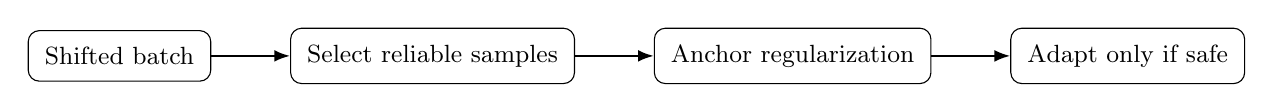
\begin{tikzpicture}[
  node distance=8mm,
  font=\small,
  box/.style={draw, rounded corners, align=center, inner sep=6pt},
  arrow/.style={-{Latex[length=2mm]}, thick}
]
\node[box] (x) {Shifted batch};
\node[box, right=10mm of x] (sel) {Select reliable samples};
\node[box, right=10mm of sel] (anc) {Anchor regularization};
\node[box, right=10mm of anc] (upd) {Adapt only if safe};
\draw[arrow] (x) -- (sel);
\draw[arrow] (sel) -- (anc);
\draw[arrow] (anc) -- (upd);
\end{tikzpicture}
}
\caption{EATA: filter out weak adaptation samples first, then regularize the remaining update.}
\end{figure}

\textbf{When to use it.}
Use EATA when false-positive adaptation is a real risk and you prefer the method to skip doubtful samples rather than force every batch to adapt.

\textbf{Concrete procedure.}
\begin{lstlisting}[language=bash]
bash scripts/ttt_compare.sh \
  --boilerplate eata \
  --dataset data/smoke \
  --split val \
  --checkpoint /path/to.ckpt \
  --run-dir reports/ttt_compare/eata \
  --device cuda
\end{lstlisting}

\textbf{Follow-up tool.}
\begin{lstlisting}[language=bash]
python3 tools/benchmark_eata_stability.py \
  --baseline reports/ttt_compare/tent/tent_predictions.json \
  --eata reports/ttt_compare/eata/eata_predictions.json \
  --output-json reports/ttt_compare/eata/eata_benchmark.json \
  --output-md reports/ttt_compare/eata/eata_benchmark.md
\end{lstlisting}

\textbf{How to read the result.}
\begin{itemize}
  \item Open \path{eata\_before\_after\_compare.md} first.
  \item If \cmd{steps\_run=0}, check the warning field before assuming anything failed.
  \item On tiny smoke subsets, \cmd{eata\_empty\_selected\_set} is expected conservative behavior.
\end{itemize}

\textbf{Concrete repo result.}
EATA has two useful examples in this repo.
On the tiny smoke fixture, it intentionally skips adaptation (\cmd{steps\_run=0}, \cmd{eata\_empty\_selected\_set}), which is conservative behavior.
On the larger fixed ten-image shifted probe, it does adapt and reaches the same small metric gain as Tent/CoTTA/SAR, as shown in Figure~\ref{fig:ttt-real-summary}.

\textbf{Pros.}
\begin{itemize}
  \item safest method when many test samples are low quality,
  \item explicit skip behavior is easy to justify operationally,
  \item anti-forgetting regularization is built into the method.
\end{itemize}

\textbf{Cons.}
\begin{itemize}
  \item may appear inactive on small subsets,
  \item harder to explain than Tent,
  \item more thresholds and diagnostics to inspect.
\end{itemize}

\subsection{SAR}
\textbf{What the name means.}
SAR refers to a \textbf{Sharpness-Aware} adaptation rule.
The key idea is to prefer updates that remain good even after a small perturbation, rather than trusting only the immediate entropy gradient.

\textbf{Principle.}
SAR performs sharpness-aware entropy minimization using a perturb-and-restore style update. Instead of trusting only the immediate entropy gradient, it prefers updates that stay stable after a small perturbation.

\textbf{Minimal objective view.}
The sharpness-aware view can be written as:
\[
\min_{\theta} \max_{\left\| \epsilon \right\| \leq \rho} L_{\mathrm{entropy}}(\theta + \epsilon).
\]
The inner perturbation asks whether the current update is fragile in a small neighborhood.
The outer step then prefers a flatter, more stable region rather than a sharp local win.

\textbf{Why it can work.}
Some shifts are noisy enough that plain entropy minimization is too eager.
SAR slows the optimizer down and asks whether the local improvement is robust, not just immediate.

\textbf{What it is not.}
\begin{itemize}
  \item It is not the cheapest method.
  \item It is not needed when Tent already behaves well.
  \item It is more about update geometry than about a stronger self-supervised signal.
\end{itemize}

\begin{figure}[h]
\centering
\resizebox{0.97\linewidth}{!}{%
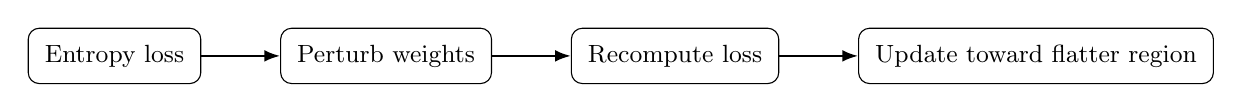
\begin{tikzpicture}[
  node distance=8mm,
  font=\small,
  box/.style={draw, rounded corners, align=center, inner sep=6pt},
  arrow/.style={-{Latex[length=2mm]}, thick}
]
\node[box] (loss1) {Entropy loss};
\node[box, right=10mm of loss1] (pert) {Perturb weights};
\node[box, right=10mm of pert] (loss2) {Recompute loss};
\node[box, right=10mm of loss2] (upd) {Update toward flatter region};
\draw[arrow] (loss1) -- (pert);
\draw[arrow] (pert) -- (loss2);
\draw[arrow] (loss2) -- (upd);
\end{tikzpicture}
}
\caption{SAR: prefer updates that remain stable after a small perturbation, not only updates that reduce the immediate entropy value.}
\end{figure}

\textbf{When to use it.}
Use SAR when the shift is noisy and you want a more conservative optimizer geometry than Tent, while accepting extra compute per update.

\textbf{Concrete procedure.}
\begin{lstlisting}[language=bash]
bash scripts/ttt_compare.sh \
  --boilerplate sar \
  --dataset data/smoke \
  --split val \
  --checkpoint /path/to.ckpt \
  --run-dir reports/ttt_compare/sar \
  --device cuda
\end{lstlisting}

\textbf{Follow-up tool.}
\begin{lstlisting}[language=bash]
python3 tools/benchmark_sar_robustness.py \
  --cotta reports/ttt_compare/cotta/cotta_predictions.json \
  --eata reports/ttt_compare/eata/eata_predictions.json \
  --sar reports/ttt_compare/sar/sar_predictions.json \
  --output-json reports/ttt_compare/sar/sar_robustness.json \
  --output-md reports/ttt_compare/sar/sar_robustness.md
\end{lstlisting}

\textbf{How to read the result.}
\begin{itemize}
  \item Open \path{sar\_before\_after\_compare.md} first.
  \item Compare runtime in \path{sar\_ttt\_log.json} against Tent to understand the extra adaptation cost.
  \item Use \path{sar\_robustness.md} when comparing SAR against CoTTA and EATA.
\end{itemize}

\textbf{Concrete repo result.}
On the fixed ten-image shifted probe, SAR reaches the same measured metric gain as Tent/CoTTA/EATA in Figure~\ref{fig:ttt-real-summary}.
For onboarding, the important point is not that SAR wins the chart, but that it lands in the same place while using a sharper, more conservative update geometry.

\textbf{Pros.}
\begin{itemize}
  \item more conservative update geometry than Tent,
  \item useful for noisy shifts,
  \item a good middle ground between Tent simplicity and CoTTA complexity.
\end{itemize}

\textbf{Cons.}
\begin{itemize}
  \item slower than Tent,
  \item conceptually harder for beginners,
  \item can be unnecessary for small or clean shifts.
\end{itemize}

\subsection{Choosing a method quickly}
\begin{center}
\begin{tabular}{p{2.1cm} p{4.1cm} p{4.1cm}}
\toprule
\textbf{Method} & \textbf{Best first use} & \textbf{Main trade-off} \\
\midrule
Tent & first ablation, safest first comparison & weakest adaptation signal \\
MIM & geometry- or pose-sensitive shift & more model-specific and harder to interpret \\
CoTTA & streaming / continual adaptation & stateful and more expensive \\
EATA & conservative adaptation with explicit skipping & may do nothing on small subsets \\
SAR & noisy shift with stability concerns & slower than Tent \\
\bottomrule
\end{tabular}
\end{center}

\subsection{Task-aware examples}
The methods above are shared, but the safest default preset depends on the task emphasis.
These examples keep the method explicit and only change the task-aware preset/auxiliary weights.

\begin{lstlisting}[language=bash,caption={Task-aware TTT examples using the same export surface.}]
# pose-heavy Tent
python3 tools/yolozu.py export \
  --backend torch --dataset reports/smoke_50 --split val \
  --checkpoint /path/to.ckpt --device cuda \
  --ttt --ttt-method tent --ttt-preset pose_safe \
  --ttt-sdft-task pose --ttt-aux-pose-weight 0.5 \
  --ttt-log-out reports/ttt_pose_safe.json \
  --output reports/pred_pose_safe.json

# keypoints-heavy Tent
python3 tools/yolozu.py export \
  --backend torch --dataset reports/smoke_50 --split val \
  --checkpoint /path/to.ckpt --device cuda \
  --ttt --ttt-method tent --ttt-preset keypoints_safe \
  --ttt-sdft-task keypoints --ttt-aux-keypoints-weight 0.5 \
  --ttt-log-out reports/ttt_keypoints_safe.json \
  --output reports/pred_keypoints_safe.json

# depth-heavy Tent
python3 tools/yolozu.py export \
  --backend torch --dataset reports/smoke_50 --split val \
  --checkpoint /path/to.ckpt --device cuda \
  --ttt --ttt-method tent --ttt-preset depth_safe \
  --ttt-sdft-task depth --ttt-aux-depth-weight 0.5 \
  --ttt-log-out reports/ttt_depth_safe.json \
  --output reports/pred_depth_safe.json

# segmentation-heavy Tent
python3 tools/yolozu.py export \
  --backend torch --dataset reports/smoke_50 --split val \
  --checkpoint /path/to.ckpt --device cuda \
  --ttt --ttt-method tent --ttt-preset seg_safe \
  --ttt-sdft-task seg --ttt-aux-seg-weight 0.5 \
  --ttt-log-out reports/ttt_seg_safe.json \
  --output reports/pred_seg_safe.json
\end{lstlisting}

\textbf{Rule of thumb.}
Start from the task-aware Tent preset, then escalate to MIM/CoTTA/EATA/SAR only when the shift evidence justifies the extra complexity and latency.

\section{YOLOZU introduction priority (high \texorpdfstring{$\to$}{->} low)}
For \yolozu{} (detection/pose), the recommended operational rollout order is:
\begin{enumerate}
  \item \textbf{CoTTA (highest priority)}: standardize \emph{teacher=EMA(model)}, use \emph{augmentation-averaged predictions} (e.g., flips) as prediction stabilization, and enable \emph{stochastic restoration} to suppress long-run drift.
  Start safely by limiting restoration and updates to \textbf{LoRA/Norm} subsets only.
  \item \textbf{EATA (second)}: add \emph{active sample selection} (only adapt on trusted samples) plus \emph{anti-forgetting regularization} (Fisher/EWC-style protection of important weights).
  In YOLOZU, constrain updates to \textbf{Norm/LoRA/selected head} parameters, and compute selection signals from detection/pose aggregates (e.g., confidence/entropy summaries across queries).
  \item \textbf{SAR (third)}: use \emph{sharpness-aware} entropy minimization for stability in wild mixed-shift / small-batch settings.
  Start with \textbf{LoRA-only} sharpness-aware updates to control cost/side effects, and prefer \textbf{GN/LN} normalization when possible (BN can be unstable under small-batch online adaptation).
\end{enumerate}

\section{CoTTA: operational design for YOLOZU (phase 1)}
This section is the phase-1 CoTTA integration scope for \yolozu{}.
The goal is to suppress long-run drift/forgetting under online test-time adaptation while keeping rollout risk low.

\subsection{Update scope (safe-by-default)}
Phase 1 restricts which parameters can change.

Allowed trainable targets:
\begin{itemize}
  \item LoRA parameters.
  \item normalization affine parameters (LN/GN/BN affine where used).
\end{itemize}

Explicitly disallowed in phase 1:
\begin{itemize}
  \item full backbone weight adaptation,
  \item unrestricted full-model optimizer updates.
\end{itemize}

\subsection{Teacher model: EMA(student)}
CoTTA uses a teacher defined as an exponential moving average (EMA) of the student parameters:
\[
\theta_{teacher} \leftarrow m\,\theta_{teacher} + (1-m)\,\theta_{student}.
\]
Teacher EMA updates run after each adaptation step, with configurable momentum $m$.
Teacher parameters are never directly optimized by gradient descent.

\subsection{Multi-augmentation prediction averaging}
Phase-1 default augmentations:
\begin{itemize}
  \item identity,
  \item horizontal flip.
\end{itemize}

Aggregation behavior:
\begin{itemize}
  \item Run the model on each augmentation branch.
  \item Map predictions back to a common image coordinate system.
  \item Aggregate with a deterministic (seed/config-pinned) confidence-aware averaging rule, then apply the standard postprocess/NMS.
\end{itemize}

\subsection{Stochastic restoration (safe mode)}
Stochastic restoration is applied only to the allowed trainable targets.
For each eligible parameter element, restore from a source snapshot with probability $p_{restore}$.
The source snapshot defaults to the initial pre-adaptation model state for the session.
Restoration executes on a configurable cadence (e.g., every $N$ adaptation steps).

\subsection{Safety boundaries and guardrails}
Phase-1 rollout requires guardrails to prevent runaway adaptation:
\begin{itemize}
  \item gradient norm clipping (\cmd{max_grad_norm}),
  \item per-step update norm cap (\cmd{max_update_norm}),
  \item cumulative update norm cap (\cmd{max_total_update_norm}),
  \item divergence stop condition via loss-ratio threshold (\cmd{max_loss_ratio}).
\end{itemize}

Failure behavior should be explicit and logged:
abort the adaptation step on hard breach, emit a diagnostics event, and restore model state according to the configured fallback policy.

\subsection{Minimum configuration knobs (phase 1)}
To keep comparisons consistent, phase-1 CoTTA should record at least:
\begin{itemize}
  \item \cmd{ttt.method=cotta}
  \item \cmd{ttt.cotta.ema_momentum}
  \item \cmd{ttt.cotta.augmentations} (initial: identity, hflip)
  \item \cmd{ttt.cotta.aggregation} (initial default: confidence-weighted mean)
  \item \cmd{ttt.cotta.restore_prob} and \cmd{ttt.cotta.restore_interval}
  \item \cmd{ttt.update_filter} (must cover norm-only, lora-only, and combined safe subset)
  \item guardrails: \cmd{ttt.max_grad_norm}, \cmd{ttt.max_update_norm}, \\
    \cmd{ttt.max_total_update_norm}, \cmd{ttt.max_loss_ratio}
\end{itemize}

\section{EATA: operational design for YOLOZU (phase 1)}
This section defines a production-safe phase-1 EATA scope for detection and pose in \yolozu{}.
The goal is to reduce unstable updates by (1) adapting only on informative samples,
(2) limiting update scope to safe parameter subsets, and (3) adding anti-forgetting regularization.

\subsection{Update scope (safe-by-default)}
Allowed trainable targets:
\begin{itemize}
  \item normalization affine parameters (LN/GN/BN affine where used),
  \item LoRA parameters,
  \item optional detection/pose head subset (explicit allowlist only; opt-in).
\end{itemize}

Explicitly disallowed in phase 1:
\begin{itemize}
  \item full backbone updates,
  \item unrestricted full-model adaptation.
\end{itemize}

Phase-1 presets should start with \cmd{norm_only} or \cmd{lora_norm_only} and keep head updates opt-in.

\subsection{Active sample selection (detection/pose aware)}
EATA adaptation steps consume only selected samples from the incoming stream.
For each image, compute selection features from prediction outputs (examples):
\begin{itemize}
  \item detection confidence aggregate (e.g., \cmd{mean_topk_conf}),
  \item detection entropy aggregate (e.g., \cmd{mean_topk_entropy}),
  \item pose confidence aggregate (e.g., \cmd{mean_kpt_conf} when keypoints exist),
  \item optional agreement score across light augmentation branches (phase-1 optional).
\end{itemize}

Phase-1 selection rule (conservative default): select a sample only when all are satisfied:
\begin{itemize}
  \item confidence lower bound: \cmd{conf \ge conf_min},
  \item entropy is within band: \cmd{entropy_min \le entropy \le entropy_max},
  \item valid detection count floor: \cmd{num_valid \ge min_valid_dets}.
\end{itemize}

\subsection{Anti-forgetting regularization (phase 1)}
Phase-1 regularization anchors online updates to the pre-adaptation snapshot.
Use a parameter-anchor penalty on the same trainable subset:
\[
L_{anchor} = \sum_i \lambda_i \left\| \theta_i - \theta_i^{(0)} \right\|_2^2.
\]

Total phase-1 objective is:
\[
L = L_{adapt} + \lambda_{anchor} L_{anchor},
\]
where $L_{adapt}$ is an entropy-based adaptation objective over selected samples.

\subsection{Safety boundaries and guardrails}
Reuse the standard TTT guardrails:
\begin{itemize}
  \item \cmd{max_grad_norm}
  \item \cmd{max_update_norm}
  \item \cmd{max_total_update_norm}
  \item \cmd{max_loss_ratio}
\end{itemize}
and rollback-on-stop behavior.

Additional EATA-specific safety checks:
\begin{itemize}
  \item minimum selected-sample ratio per step (\cmd{selected_ratio_min}),
  \item skip-step when the selected set is empty,
  \item max consecutive skipped steps (\cmd{max_skip_streak}) to trigger early stop with warning.
\end{itemize}

\subsection{Minimum configuration knobs (phase 1)}
Phase-1 EATA should record at least:
\begin{itemize}
  \item \cmd{ttt.method=eata}
  \item \cmd{ttt.update_filter} (\cmd{norm_only}, \cmd{lora_only}, \cmd{lora_norm_only}, optional head allowlist)
  \item thresholds: \\
    \cmd{ttt.eata.conf_min}, \\
    \cmd{ttt.eata.entropy_min}, \\
    \cmd{ttt.eata.entropy_max}, \\
    \cmd{ttt.eata.min_valid_dets}
  \item anchor: \cmd{ttt.eata.anchor_lambda}
  \item selection safety: \cmd{ttt.eata.selected_ratio_min}, \cmd{ttt.eata.max_skip_streak}
  \item guardrails: \cmd{ttt.max_grad_norm}, \cmd{ttt.max_update_norm}, \\
    \cmd{ttt.max_total_update_norm}, \cmd{ttt.max_loss_ratio}
\end{itemize}

\section{SAR: operational design for YOLOZU (phase 1)}
This section defines a production-safe phase-1 SAR rollout scope for \yolozu{}.
The goal is to improve robustness under challenging distribution shifts by introducing sharpness-aware entropy minimization
with controlled update scope.

\subsection{Update scope (LoRA-only by default)}
Allowed update targets:
\begin{itemize}
  \item LoRA parameters only (default).
  \item optional norm affine subset in controlled experiments (not default).
\end{itemize}

Explicitly disallowed in phase 1:
\begin{itemize}
  \item full-backbone sharpness-aware updates,
  \item unrestricted full-model SAM-style optimization.
\end{itemize}

\subsection{Optimization behavior (sharpness-aware entropy)}
Phase-1 SAR uses a two-stage sharpness-aware update over the selected trainable parameters:
\begin{enumerate}
  \item compute gradient on the entropy objective,
  \item perturb weights along a normalized gradient direction,
  \item compute a second loss at the perturbed point,
  \item apply the optimizer update on the original weights.
\end{enumerate}

Conceptually:
\[
\min_{\theta} \max_{\left\| \epsilon \right\| \leq \rho} L_{entropy}(\theta + \epsilon),
\]
with $\rho$ bounded conservatively for phase 1.

\subsection{Normalization policy guidance}
If SAR experiments require normalization updates:
\begin{itemize}
  \item prefer GN/LN-first configurations,
  \item avoid BN-stat-heavy behavior in tiny/unstable batches,
  \item keep BN running-stat side effects monitored and rollback-capable.
\end{itemize}
Default rollout remains LoRA-only.

\subsection{Safety boundaries and expected costs}
Expected cost profile:
approximately $\sim$2x forward/backward cost per adaptation step versus single-step entropy update,
plus extra memory traffic due to perturb-and-restore.

Required safeguards:
strict gradient/update caps, immediate rollback on guardrail breach, explicit stop-reason logging,
and conservative default \cmd{steps=1} and \cmd{max_batches=1}.

\subsection{Minimum configuration knobs (phase 1)}
Phase-1 SAR should record at least:
\begin{itemize}
  \item \cmd{ttt.method=sar}
  \item \cmd{ttt.update_filter} defaulting to \cmd{lora_only}
  \item \cmd{ttt.sar.rho}, \cmd{ttt.sar.adaptive}, \cmd{ttt.sar.first_step_scale}
  \item guardrails: \cmd{ttt.max_grad_norm}, \cmd{ttt.max_update_norm}, \\
    \cmd{ttt.max_total_update_norm}, \cmd{ttt.max_loss_ratio}
\end{itemize}

\section{Guard rails (safety limits)}
If you do not explicitly set these, defaults are applied by preset:
\begin{itemize}
  \item \cmd{max_grad_norm}
  \item \cmd{max_update_norm}
  \item \cmd{max_total_update_norm}
  \item \cmd{max_loss_ratio}
\end{itemize}

These bounds are there to prevent runaway adaptation and to keep comparisons reproducible.

\section{Reset policy: stream vs sample}
\begin{description}
  \item[\cmd{--ttt-reset stream}] Adapt once (up to \cmd{--ttt-max-batches}) then reuse adapted weights for subsequent images.
  \item[\cmd{--ttt-reset sample}] Restore base state per image, adapt on that image/batch, then predict. Slower but cleaner ablations.
\end{description}

\begin{figure}[h]
\centering
\resizebox{\linewidth}{!}{%
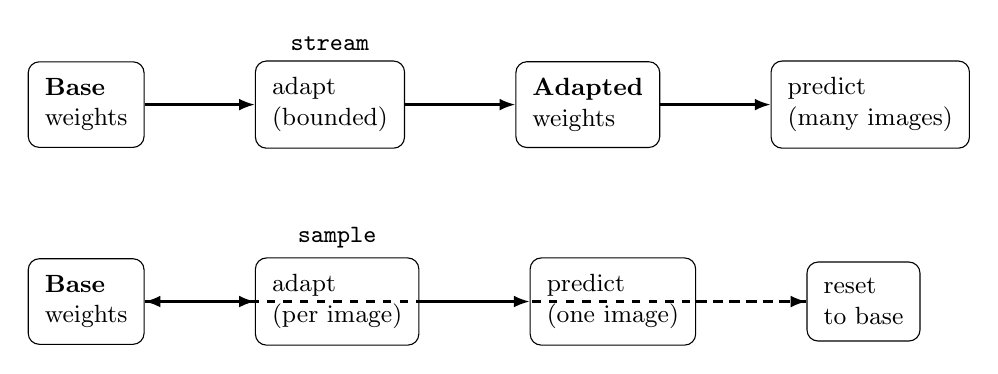
\begin{tikzpicture}[
  node distance=10mm,
  font=\small,
  box/.style={draw, rounded corners, align=left, inner sep=6pt},
  arrow/.style={-{Latex[length=2mm]}, thick},
  dashedarrow/.style={-{Latex[length=2mm]}, thick, dashed}
]

% Stream row
\node[box] (s0) {\textbf{Base}\\weights};
\node[box, right=14mm of s0, label={[font=\small]above:\cmd{stream}}] (s1) {adapt\\(bounded)};
\node[box, right=14mm of s1] (s2) {\textbf{Adapted}\\weights};
\node[box, right=14mm of s2] (s3) {predict\\(many images)};
\draw[arrow] (s0) -- (s1);
\draw[arrow] (s1) -- (s2);
\draw[arrow] (s2) -- (s3);

\node[box, below=14mm of s0] (p0) {\textbf{Base}\\weights};
\node[box, right=14mm of p0, label={[font=\small]above:\cmd{sample}}] (p1) {adapt\\(per image)};
\node[box, right=14mm of p1] (p2) {predict\\(one image)};
\node[box, right=14mm of p2] (p3) {reset\\to base};
\draw[arrow] (p0) -- (p1);
\draw[arrow] (p1) -- (p2);
\draw[dashedarrow] (p2) -- (p3);
\draw[dashedarrow] (p3) -- (p0);

\end{tikzpicture}
}
\caption{Reset policies: \cmd{stream} keeps adapted state across images; \cmd{sample} resets per image for clean ablations.}
\end{figure}

For plots and controlled comparisons, start with \cmd{--ttt-reset sample}.

\section{Bounded-cost knobs}
Two knobs matter most for runtime and fairness:
\begin{itemize}
  \item \cmd{--ttt-batch-size N}: images per adaptation step.
  \item \cmd{--ttt-max-batches K}: hard cap on adaptation batches consumed.
\end{itemize}

Suggested smoke-test settings:
\cmd{--ttt-batch-size 1 --ttt-max-batches 1}.

\section{Method switch (manifest-aligned)}
TTT method can be selected with \cmd{--ttt-method}:
\begin{itemize}
  \item \cmd{tent}
  \item \cmd{mim}
  \item \cmd{cotta}
  \item \cmd{eata}
  \item \cmd{sar}
\end{itemize}

The current canonical CLI surface is reflected in \path{tools/manifest.json}
for \path{tools/export_predictions.py} and \path{tools/yolozu.py}.

\section{Make a fixed evaluation subset}
TTT comparisons must be run on the exact same images.
Use \path{tools/make_subset_dataset.py} to create a deterministic subset dataset root:
\begin{lstlisting}[language=bash]
python3 tools/make_subset_dataset.py \
  --dataset data/smoke \
  --split val \
  --n 50 \
  --seed 0 \
  --out reports/smoke_50
\end{lstlisting}

This writes \path{subset.json} (including an image hash) and a frozen image list.

\section{Example: baseline vs TTT}
Baseline export:
\begin{lstlisting}[language=bash]
python3 tools/yolozu.py export \
  --backend torch \
  --dataset reports/smoke_50 \
  --split val \
  --checkpoint /path/to.ckpt \
  --device cuda \
  --max-images 50 \
  --output reports/pred_baseline.json
\end{lstlisting}

TTT export (safe preset, per-sample reset, with a log):
\begin{lstlisting}[language=bash]
python3 tools/yolozu.py export \
  --backend torch \
  --dataset reports/smoke_50 \
  --split val \
  --checkpoint /path/to.ckpt \
  --device cuda \
  --max-images 50 \
  --ttt \
  --ttt-preset safe \
  --ttt-reset sample \
  --ttt-log-out reports/ttt_log_safe.json \
  --output reports/pred_ttt_safe.json
\end{lstlisting}

\section{MIM-based adaptation (high level)}
The geometry-aligned MIM branch (when enabled in the model) can be used for test-time adaptation.
Conceptually:
\begin{itemize}
  \item Use geometry-derived features as a teacher (mask + normalized depth).
  \item Reconstruct masked features (MIM/MAE-style) \cite{he2022mae,xie2022simmim} and optionally minimize entropy \cite{grandvalet2005entropy}.
  \item Update a restricted parameter subset (e.g., norm or adapter/head) under guard rails.
\end{itemize}

Conceptually, MIM-style inference adds an auxiliary loss (computed at inference time) to adapt parameters or latent state under distribution shift.
In this repo, the important operational points are:
\begin{itemize}
  \item keep the loss bounded and the update schedule explicit,
  \item record adaptation settings into run artifacts,
  \item compare against a non-adapted baseline under the same pinned evaluation protocol.
\end{itemize}

\section{Operational notes}
\begin{itemize}
  \item TTT adds latency. Always report throughput and the chosen \cmd{batch_size/max_batches}.
  \item Keep the evaluation subset fixed and record the exact preset and guards.
  \item For deployment, treat TTT as an optional mode; default inference should not require it.
\end{itemize}

\section{Method-specific evaluation tools}
Manifest-registered benchmark tools for TTT phase validation:
\begin{itemize}
  \item \path{tools/eval_cotta_drift.py} (baseline vs CoTTA drift/stability)
  \item \path{tools/benchmark_eata_stability.py} (baseline vs EATA stability/efficiency)
  \item \path{tools/benchmark_sar_robustness.py} (SAR vs CoTTA/EATA go/no-go impact)
\end{itemize}

These tools emit reproducible JSON/Markdown evidence artifacts and should be preferred over ad-hoc notebook-only comparisons.


\part{Maintainer, Automation, and Appendices}
\chapter{Tool Registry and Automation (Research Use)}

\ChapterMeta{
This chapter elucidates the machine-readable tool registry (comprising the manifest and schemas) and its role in facilitating safe discovery and execution for both human operators and autonomous agents.
}{
It underpins reproducible automation and Continuous Integration (CI)-style workflows by strictly pinning tool I/O interface contracts and validating the registry's surface area.
}{
This documentation assumes that tools are invoked exclusively via their declared entrypoints and validated using \cmd{python3 tools/validate_tool_manifest.py}. Path-resolution rules are critical for robust automation.
}
\ChapterAudience{Read this chapter when you maintain tools, automation, or manifest-driven documentation and need the operational source of truth.}


\section{The Rationale for a Tool Registry}
Research workflows frequently accumulate disparate scripts. \yolozu{} addresses this by treating the \path{tools/} directory as a stable, scriptable interface layer, augmented by a machine-readable registry:
\begin{itemize}
  \item \textbf{Tool Manifest}: \path{tools/manifest.json}
  \item \textbf{Manifest Schema}: \path{docs/schemas/tools_manifest.schema.json}
  \item \textbf{Validator}: \cmd{python3 tools/validate_tool_manifest.py}
\end{itemize}

This architecture is explicitly designed to serve:
\begin{itemize}
  \item \textbf{Human Operators}: Providing a clear answer to "What command do I run to achieve X?"
  \item \textbf{Agentic Automation}: Enabling safe, programmatic discovery of entrypoints and I/O interface contracts.
  \item \textbf{CI-Style Reproducibility}: Ensuring stable commands and deterministic artifact generation.
\end{itemize}

\section{Authority and the Update Imperative}
For CLI capabilities and tool I/O behavior, \path{tools/manifest.json} serves as the \textbf{authoritative source of truth}. Manual documentation must be synchronized from the manifest, rather than maintained as an independent, potentially divergent list.

In the event of a discrepancy:
\begin{itemize}
  \item \textbf{Behavioral Truth}: Resides in the code and the manifest.
  \item \textbf{Documentation Action}: Update this manual chapter and any related chapters to reflect the manifest.
  \item \textbf{Quality Gate}: Re-run the manifest validator prior to publishing any changes.
\end{itemize}

Execute the following command to verify compliance:
\begin{lstlisting}[language=bash]
python3 tools/validate_tool_manifest.py --manifest tools/manifest.json --require-declarative
\end{lstlisting}

\section{Declarative Fields: Mandatory Tool Metadata}
The manifest functions as a declarative interface contract. At a practical minimum, every tool entry must expose:
\begin{itemize}
  \item \textbf{Identity and Execution}: \texttt{id}, \texttt{entrypoint}, \texttt{runner}, \texttt{summary}, and \texttt{maturity}.
  \item \textbf{Environment}: \texttt{platform} constraints and optional \texttt{requires} dependencies.
  \item \textbf{Interface}: Explicit \texttt{inputs[]} and \texttt{outputs[]} definitions.
  \item \textbf{Side Effects}: Declared \texttt{effects.writes[]} and \texttt{effects.fixed\_writes[]}.
  \item \textbf{Reproducibility}: At least one functional \texttt{examples[].command}.
  \item \textbf{Typing and Compatibility}: \texttt{contracts.consumes} and \texttt{contracts.produces}, alongside optional \texttt{contract\_outputs} and \texttt{docs[]} references.
\end{itemize}

For comprehensive field-level policies and boundaries, consult \path{docs/manifest_declarative_spec.md}.

\section{Contracts Referenced by the Manifest}
The manifest references stable JSON schemas located under \path{docs/schemas/}. Prominent schemas include:
\begin{itemize}
  \item \textbf{Predictions}: \path{docs/schemas/predictions.schema.json}
  \item \textbf{Evaluation Suite Reports}: \path{docs/schemas/eval_suite_report.schema.json}
  \item \textbf{COCO Evaluation Reports}: \path{docs/schemas/coco_eval_report.schema.json}
  \item \textbf{Segmentation}: Schemas for both semantic and instance segmentation predictions and evaluation reports.
\end{itemize}

In a research context, these schemas are invaluable as they drastically reduce the overhead required to:
\begin{itemize}
  \item Parse and aggregate results across numerous experimental runs.
  \item Construct dashboards and visualizations from JSONL histories.
  \item Implement assertions (regression gates) against strictly typed outputs.
\end{itemize}

\section{The Discovery Loop}
A recommended practical loop when onboarding to the repository (or returning after an absence):
\begin{enumerate}
  \item Review the documentation index: \path{docs/README.md}.
  \item Scan the tool index: \path{docs/tools_index.md}.
  \item Query the manifest by \texttt{tags}, \texttt{id}, and \texttt{contracts}.
  \item Execute the validator to ensure the registry remains trustworthy.
\end{enumerate}

\subsection*{Practical Manifest Queries}
\begin{lstlisting}[language=bash]
# List all tool IDs and their corresponding entrypoints
python3 - <<'PY'
import json
with open("tools/manifest.json", "r", encoding="utf-8") as f:
    manifest = json.load(f)
for tool in manifest.get("tools", []):
    print(f"{tool.get('id')}\t{tool.get('entrypoint')}")
PY

# Identify tools that consume the 'predictions_json' contract
python3 - <<'PY'
import json
with open("tools/manifest.json", "r", encoding="utf-8") as f:
    manifest = json.load(f)
for tool in manifest.get("tools", []):
    consumes = (tool.get("contracts") or {}).get("consumes", [])
    if "predictions_json" in consumes:
        print(tool.get("id"))
PY
\end{lstlisting}

\section{AI-First Entrypoints for Autonomous Agents}
For autonomous or semi-autonomous operations, the recommended stable entrypoints are:
\begin{itemize}
  \item \textbf{Canonical CLI}: \cmd{yolozu --help} (or \cmd{python3 -m yolozu --help})
  \item \textbf{Tool Registry}: \path{tools/manifest.json}
  \item \textbf{Contracts and Schemas}: \path{docs/schemas/*.schema.json}
  \item \textbf{Usage Guide}: \path{docs/ai_first.md}
\end{itemize}

This represents an explicit design objective of \yolozu{}: AI agents must be capable of discovering, validating, executing, and extending workflows utilizing stable, well-defined interface contracts.

\section{Manifest-Synchronized Documentation Workflow}
When introducing or modifying a tool, adhere to the following workflow:
\begin{enumerate}
  \item Update the script's behavior within \path{tools/} and ensure the CLI help output remains accurate.
  \item Update \path{tools/manifest.json} to reflect changes in inputs, effects, outputs, examples, and contracts.
  \item Validate the manifest's structure and internal references.
  \item Revise the corresponding manual chapter sections and examples.
  \item Maintain synchronization of documentation links (e.g., \path{docs/README.md}, \path{docs/tools_index.md}).
\end{enumerate}

This rigorous process keeps manual chapters aligned with the registry, thereby minimizing stale command drift.

Validate the tool registry using:
\begin{lstlisting}[language=bash]
python3 tools/validate_tool_manifest.py --manifest tools/manifest.json --require-declarative
\end{lstlisting}

\subsection*{SynthGen intake tools (registry additions)}
The registry now exposes explicit intake utilities for externally generated synthetic shards:
\begin{itemize}
  \item \cmd{validate_synthgen_contract}: validate required SynthGen fields and tensor/range constraints.
  \item \cmd{render_synthgen_overlay}: generate semantic/instance/keypoint debug overlays.
  \item \cmd{eval_synthgen}: compute keypoint, segmentation, and depth summaries for SynthGen predictions.
  \item \cmd{smoke_synthgen}: run a deterministic interface-contract+overlay+eval smoke pass on \path{data/smoke/synthgen_minishard}.
\end{itemize}

These tools reference the canonical SynthGen interface contract at \path{docs/synthgen_contract.md} and \path{schemas/synthgen_sample.schema.json}.

\subsection*{TTT figure renderer (registry addition)}
The registry also exposes \cmd{render_ttt_manual_figures}, which regenerates:
\begin{itemize}
  \item \path{docs/assets/ttt_method_results_summary.png}
  \item \path{docs/assets/ttt_compare_pipeline.png}
  \item \path{docs/assets/ttt_probe_example_panel.png}
\end{itemize}

This keeps the TTT chapter's beginner-facing PNG figures reproducible and synchronized with fixed result artifacts rather than hand-edited screenshots.

\section{Release Automation: Manual PDF DOI as a Separate Record}
For release operations, YOLOZU intentionally keeps software DOI and manual DOI lifecycles independent:
\begin{itemize}
  \item Software release and PyPI publish are handled by \path{.github/workflows/publish.yml}.
  \item Manual PDF DOI publishing is handled by \path{.github/workflows/manual_doi.yml}.
\end{itemize}

The software publish workflow now enforces release metadata consistency before PyPI publish:
\begin{itemize}
  \item release-triggered runs validate that tag \cmd{vX.Y.Z} matches \path{yolozu/__init__.py}
  \item manual \cmd{workflow_dispatch} runs require \cmd{expected_version}
  \item optional manual input \cmd{release_tag} can re-check tag/version alignment during recovery
  \item \path{CHANGELOG.md} must contain a matching \cmd{## [X.Y.Z] - YYYY-MM-DD} section
\end{itemize}

Operational helper script (no required options):
\begin{lstlisting}[language=bash]
bash release.sh
\end{lstlisting}

Versioning policy is automatic:
\begin{itemize}
  \item Current \texttt{X.Y.Z}: SemVer bump based on release size.
  \item Current \texttt{YYYY.MM.DD.MICRO}: CalVer bump with same-day micro increment and UTC-day rollover reset.
\end{itemize}

Dry-run preview:
\begin{lstlisting}[language=bash]
bash release.sh --dry-run --allow-dirty --allow-non-main --output reports/release_report.dry_run.json
\end{lstlisting}

When operators need to recover a failed publish without cutting a new tag, the supported path is the
\path{publish.yml} manual trigger with:
\begin{itemize}
  \item \texttt{expected\_version = X.Y.Z}
  \item optional \texttt{release\_tag = vX.Y.Z}
\end{itemize}
This keeps the PyPI publish path explicit instead of allowing a loosely-scoped manual rerun.

The manual DOI workflow builds \path{manual/build/yolozu_manual.pdf} and publishes it to Zenodo either as:
\begin{itemize}
  \item a new version (\texttt{actions/newversion}) when a manual \texttt{conceptrecid} is configured, or
  \item a first deposition when no prior concept record exists.
\end{itemize}

To preserve machine-readable linkage between records, manual metadata sets:
\begin{itemize}
  \item \texttt{related\_identifiers[].relation = isSupplementTo}
  \item \texttt{related\_identifiers[].scheme = doi}
  \item \texttt{related\_identifiers[].identifier =} software concept DOI
\end{itemize}

Operationally, configure repository variables:
\begin{itemize}
  \item \texttt{YOLOZU\_SOFTWARE\_CONCEPT\_DOI} (required)
  \item \texttt{YOLOZU\_MANUAL\_CONCEPTRECID} (recommended for versioned manual updates)
\end{itemize}

\section{Path Resolution Behavior (Critical for Automation)}
Many tools adhere to consistent path resolution rules (summarized in \path{docs/tools_index.md} and \path{docs/ai_first.md}):
\begin{itemize}
  \item CLI-relative input paths resolve from the current working directory.
  \item Config-relative paths (where supported) resolve from the directory containing the configuration file.
  \item Relative outputs are written relative to the current working directory.
\end{itemize}

\section{Safety Guardrails for Agentic Write Actions}
Prior to writing artifacts or mutating state, agents and users should prioritize:
\begin{itemize}
  \item Utilizing \textbf{dry-run modes} wherever available.
  \item Applying \textbf{explicit caps or ranges} (e.g., \cmd{--max-images}) to limit execution scope.
  \item Directing outputs to \textbf{deterministic locations}, such as under \path{reports/} or a dedicated run directory.
\end{itemize}

In a research environment, these practices ensure that batch operations run reliably across different working directories and enhance the portability of scripted executions.

\include{chapters/18_manifest_driven_docs}
\chapter{LLM MCP Integrations (Gemini / Claude / Copilot / OpenAI)}
\ChapterMeta{Scope:}{}
{Unified MCP-first integration strategy across major LLM clients.}

\section{Principle: one backend, many clients}

All clients should share the same implementation backend:

\begin{lstlisting}[language=bash]
python3 tools/run_mcp_server.py
\end{lstlisting}

Core exposed tools:
\begin{itemize}
  \item \cmd{doctor}
  \item \cmd{generate\_config}
  \item \cmd{review\_config}
  \item \cmd{validate\_predictions}
  \item \cmd{validate\_dataset}
  \item \cmd{eval\_coco}
  \item \cmd{run\_scenarios}
  \item \cmd{convert\_dataset} (optional)
\end{itemize}

Return payload policy (for all clients):
\begin{itemize}
  \item machine-readable JSON
  \item short textual summary in \cmd{summary}
  \item stable top-level keys: \cmd{ok}, \cmd{tool}, \cmd{summary}, \cmd{exit\_code}
  \item optional metadata: \cmd{meta.git\_sha}, \cmd{meta.manifest\_sha256}, runtime details
\end{itemize}

\section{Layer model (fixed)}

\begin{enumerate}
  \item Core layer: I/O envelope, auth/log hooks, error shaping.
  \item YOLOZU API layer: CLI/Python wrapper, argument normalization, manifest resolution.
  \item Job layer: long-running operations with \cmd{job\_id} tracking.
  \item Artifact layer: run artifacts and metadata return (git SHA / manifest hash / environment).
\end{enumerate}

\section{Quick start (MCP + Actions API)}

\subsection{MCP server}
\begin{lstlisting}[language=bash]
python3 tools/run_mcp_server.py
\end{lstlisting}

Official MCP Lite surface (deterministic, intended for AI-safe clients):
\begin{itemize}
  \item \cmd{doctor}
  \item \cmd{generate\_config}
  \item \cmd{review\_config}
\end{itemize}

Copy-paste sanity checks:
\begin{lstlisting}[language=bash]
python3 tools/run_mcp_server.py --print-tools > reports/mcp_tools.json
python3 tools/run_mcp_server.py --sample-generate-config > reports/ai_generate_config.json
python3 tools/run_mcp_server.py --sample-review-config reports/ai_generate_config.json > reports/ai_review_config.json
\end{lstlisting}

\subsection{Actions API (optional route)}
\begin{lstlisting}[language=bash]
python3 tools/run_actions_api.py --host 127.0.0.1 --port 8080 --workers 1
curl -sS http://127.0.0.1:8080/healthz
\end{lstlisting}

\subsection{Minimal end-to-end check}
\begin{lstlisting}[language=bash]
python3 tools/yolozu.py doctor --output reports/doctor.json
python3 tools/yolozu.py validate predictions data/smoke/predictions/predictions_dummy.json --strict
python3 tools/yolozu.py eval-coco --dataset data/smoke --predictions data/smoke/predictions/predictions_dummy.json --dry-run --output reports/mcp_eval_coco_dry.json
\end{lstlisting}

\section{Client routing}

\subsection{Gemini}
Use MCP first. Optionally use API tool-calling via OpenAPI endpoint.

\subsection{Claude}
Use MCP first with thin prompt wrappers; avoid duplicating tool logic.

\subsection{Copilot}
Use Copilot Extensions / VS Code participant that calls MCP backend (or API fallback).

\subsection{OpenAI}
Use MCP first; add GPT Actions when OpenAPI registration is required.

Optional API route:
\begin{lstlisting}[language=bash]
python3 tools/run_actions_api.py --host 127.0.0.1 --port 8080 --workers 1
# OpenAPI: http://127.0.0.1:8080/openapi.json
\end{lstlisting}

\subsection{Ollama (local LLM)}
Ollama runs models locally and can be used as the reasoning engine behind an MCP-capable client.
The \yolozu{} backend does not change: keep using the same \yolozu{} MCP server.

Start (or confirm) Ollama is running:
\begin{lstlisting}[language=bash]
ollama serve
ollama pull llama3.1
\end{lstlisting}

Then configure your client runtime to use Ollama as an \textbf{OpenAI-compatible} endpoint:
\begin{lstlisting}[language=bash]
# Typical values (client-dependent)
OPENAI_BASE_URL=http://127.0.0.1:11434/v1
OPENAI_API_KEY=ollama

# Example model identifiers are Ollama-local names
OPENAI_MODEL=llama3.1
\end{lstlisting}

Optional sanity checks:
\begin{lstlisting}[language=bash]
# Native Ollama API
curl -sS http://127.0.0.1:11434/api/tags

# OpenAI-compatible API
curl -sS http://127.0.0.1:11434/v1/models
\end{lstlisting}

Notes:
\begin{itemize}
  \item MCP tool execution still routes to \cmd{python3 tools/run\_mcp\_server.py}; only the LLM provider/model changes.
  \item Environment variable names are client-specific; some clients use \cmd{OPENAI\_API\_BASE} instead of \cmd{OPENAI\_BASE\_URL}.
  \item Model capability varies by local weights; if tool selection is unstable, prefer a stronger local model and keep prompts/tool wrappers thin.
  \item Verify the endpoint is reachable via \cmd{http://127.0.0.1:11434/v1/models} (OpenAI-compatible) in environments that support it.
\end{itemize}

\section{Operational recommendation}

Maintain feature parity by implementing behavior once in backend runner and exposing it through MCP/API adapters.

Operational guards in v2 layer implementation:
\begin{itemize}
  \item Allowlist is manifest-first (\path{tools/manifest.json}) with conservative fallback defaults.
  \item Path tokens are guarded (\cmd{..} rejected; absolute paths outside workspace rejected).
  \item Job state persistence to \cmd{runs/mcp\_jobs/*.json} for restart-safe status retrieval.
  \item Stale in-flight states (queued/running after restart) are surfaced as \cmd{unknown}.
  \item CLI execution timeout and output-size caps with explicit truncation metadata.
\end{itemize}

\section{Tool map (actual MCP/Actions surface)}

\subsection{Official support boundary (1.0.x)}
\begin{itemize}
  \item Guaranteed (deterministic/lightweight): \cmd{doctor}, \cmd{generate\_config}, \cmd{review\_config}, \cmd{validate\_predictions}
  \item Best-effort (environment dependent): long training jobs, TensorRT build/export, OpenCV CUDA/OpenVINO backends
\end{itemize}

\subsection{Synchronous tools}
\begin{itemize}
  \item Data/validation: \cmd{doctor}, \cmd{validate\_predictions}, \cmd{validate\_dataset}, \cmd{convert\_dataset}
  \item Inference/calibration: \cmd{predict\_images}, \cmd{parity\_check}, \cmd{calibrate\_predictions}
  \item Evaluation: \cmd{eval\_coco}, \cmd{eval\_instance\_seg}, \cmd{eval\_long\_tail}, \cmd{run\_scenarios}
\end{itemize}

\subsection{Asynchronous job tools}
\begin{itemize}
  \item \cmd{train\_job}, \cmd{export\_predictions\_job}, \cmd{test\_job}, \cmd{ttt\_job}, \cmd{ctta\_job}
  \item compatibility alias: \cmd{export\_onnx\_job} (same behavior as \cmd{export\_predictions\_job})
  \item control/query: \cmd{jobs.list}, \cmd{jobs.status}, \cmd{jobs.cancel}, \cmd{runs.list}, \cmd{runs.describe}
\end{itemize}

\section{AI operation pitfalls (high-impact)}

\begin{enumerate}
  \item Always pass \cmd{dataset} as a YOLO root and specify \cmd{split} explicitly.
  \item Prefer workspace-relative paths to avoid API-layer path guard rejections.
  \item Treat \cmd{ok/tool/summary/exit\_code} as the canonical status contract.
  \item For long tasks, do not poll stdout; use \cmd{job\_id} with \cmd{jobs.status}.
  \item Assume post-restart in-flight jobs become \cmd{unknown}; requeue deterministically if needed.
  \item Set \cmd{dry\_run}/\cmd{strict}/\cmd{force} explicitly to avoid client-default drift.
\end{enumerate}

\section{Efficiency backlog for MCP hardening}

High-value follow-ups that reduce AI ambiguity and integration drift:
\begin{itemize}
  \item Generated MCP/Actions reference now lives at:
  \begin{itemize}
    \item \path{docs/generated/mcp\_actions\_tool\_reference.json}
    \item \path{docs/generated/mcp\_actions\_tool\_reference.md}
  \end{itemize}
  \item Regenerate/check command: \cmd{python3 tools/generate\_integration\_tool\_reference.py --check}
  \item Add explicit error-code taxonomy for allowlist/path/timeout failures in integration responses.
\end{itemize}

\section{CI no-abandon policy}

For MCP-related changes:
\begin{enumerate}
  \item Run local validation (manifest + tests).
  \item Push and monitor latest CI result.
  \item If failed, patch immediately and rerun until green.
\end{enumerate}

\section{Cross references}

\begin{itemize}
  \item OpenAI details: \cmd{docs/openai\_mcp\_actions.md}
  \item Copilot details: \cmd{docs/copilot\_mcp\_integration.md}
  \item Shared overview: \cmd{docs/llm\_integrations.md}
\end{itemize}

\chapter{SynthGen Repo Integration}
\ChapterMeta{
This chapter defines the repo-to-repo handoff between an external generator such as \path{YOLOZU-synthgen} and \yolozu{}.
}{
It keeps the integration boundary small: the generator owns rendering and shard creation, while \yolozu{} owns validation, overlay inspection, and evaluation.
}{
The practical goal is to make a synthetic dataset handoff reproducible, CI-friendly, and easy to verify before training work begins.
}
\ChapterAudience{Read this chapter when you are connecting \path{YOLOZU-synthgen} or another external synthetic-data generator to the YOLOZU intake and evaluation path.}

\section{Boundary and ownership}

The shared boundary is the SynthGen sample interface contract:
\begin{itemize}
  \item Spec: \path{docs/synthgen_contract.md}
  \item JSON Schema: \path{schemas/synthgen_sample.schema.json}
  \item Runtime validator: \path{yolozu/contracts/synthgen.py}
\end{itemize}

Ownership split:
\begin{itemize}
  \item External generator repo: prompts, asset selection, rendering, shard creation, generator metadata
  \item \yolozu{}: interface-contract validation, shard loading, overlay rendering, evaluation, smoke checks
\end{itemize}

Each record in \path{shards/*.jsonl} must satisfy \cmd{schema\_version="1"} and provide the required tensors and metadata fields used by the intake adapters.

\section{Recommended dataset root}

\begin{lstlisting}
<dataset-root>/
  shards/
    train_000.jsonl
    predictions_synthgen.json
  <sample>_image.png
  <sample>_depth.npy
  <sample>_inst.npy
  <sample>_sem.npy
  <sample>_kpts.npy
\end{lstlisting}

Practical note: if the predictions artifact reuses shard-relative asset paths such as \path{../samples/...}, keep that predictions JSON under \path{shards/} so the relative base remains the same as the shard rows. If you prefer to store predictions elsewhere, rewrite those asset paths first.

\section{Verified cross-repo probe}

This handoff was exercised end to end on April 2, 2026 using a local \path{YOLOZU-synthgen} checkout and the CPU path. GPU or MPS support is not required for these intake checks.

\subsection{Generator-side commands}

\begin{lstlisting}[language=bash]
PYTHONPATH=src ./.venv/bin/python -m yolozu_synthgen generate-demo-dataset \
  --output-dir /tmp/yolozu_synthgen_demo \
  --num-train 2 \
  --num-val 1

PYTHONPATH=src ./.venv/bin/python -m yolozu_synthgen export-yolozu-synthgen \
  --shards-root /tmp/yolozu_synthgen_demo/shards \
  --output-dir /tmp/yolozu_synthgen_export
\end{lstlisting}

\subsection{YOLOZU-side acceptance checks}

\begin{lstlisting}[language=bash]
python3 tools/validate_synthgen_contract.py \
  --input /tmp/yolozu_synthgen_export/shards/train_000.jsonl \
  --max-samples 20

python3 tools/render_synthgen_overlay.py \
  --dataset-root /tmp/yolozu_synthgen_export \
  --schema-id animal_v1 \
  --sample-index 0 \
  --output /tmp/yolozu_synthgen_overlay.png

python3 tools/eval_synthgen.py \
  --dataset-root /tmp/yolozu_synthgen_export \
  --predictions /tmp/yolozu_synthgen_export/shards/predictions_synthgen.json \
  --schema-id animal_v1 \
  --output /tmp/yolozu_synthgen_eval.json

python3 tools/smoke_synthgen.py \
  --dataset-root /tmp/yolozu_synthgen_export \
  --predictions /tmp/yolozu_synthgen_export/shards/predictions_synthgen.json \
  --output-dir /tmp/yolozu_synthgen_smoke
\end{lstlisting}

\section{Acceptance criteria}

The handoff is ready when all of the following are true:
\begin{itemize}
  \item \cmd{validate\_synthgen\_contract.py} returns \texttt{OK}
  \item \cmd{render\_synthgen\_overlay.py} writes a non-empty overlay image
  \item \cmd{eval\_synthgen.py} writes a report JSON without schema or shape errors
  \item \cmd{smoke\_synthgen.py} writes overlay, eval, and summary artifacts under the chosen output directory
\end{itemize}

\section{Versioning rule}

\begin{itemize}
  \item Add optional fields freely.
  \item Add new \cmd{schema\_id} values freely.
  \item Do not change required dtype, shape, or range semantics inside \cmd{schema\_version="1"}.
  \item If the generator needs a breaking change, version the interface contract in \yolozu{} first, then enable it in adapters and docs.
\end{itemize}


\appendix
\include{chapters/19_appendix_dependency_graphs}

\IfFileExists{references.bib}{%
  \clearpage
  \renewcommand{\bibname}{References}
  \phantomsection
  \addcontentsline{toc}{chapter}{References}
  \nocite{*}
  \bibliographystyle{plain}
  \bibliography{references}
}{}

\end{document}
